\documentclass[a4paper,oneside,hidelinks]{Tptesi2}

\usepackage[italian]{babel}
\usepackage{listings}
\usepackage{amsmath,amssymb}
\usepackage{verbatim}
\usepackage{bigstrut}
\usepackage{transparent}
\usepackage{indentfirst}
\usepackage{subfigure}
\usepackage{algorithmic}
\usepackage{framed}
\usepackage{rotating}
\usepackage{cite}
\usepackage[figurename=Figura]{caption}

% Packages -----------------------------------------------------------------------
%\usepackage{amsthm}
%\usepackage{amsmath}          % Non necessario se usi TPTESI2 perche' gia` incluso
%\usepackage[dvips]{graphicx}  % Non necessario se usi TPTESI2 perche' gia` incluso
%\usepackage{url} %non usare se si usa hyperref


\newcommand{\mr}{\emph{motore di ricerca}}
\newcommand{\Mr}{\emph{Motore di ricerca}}
\newcommand{\ws}{Web~service }


% Use a small font for the verbatim environment
\makeatletter  % makes '@' an ordinary character
\renewcommand{\verbatim@font}{%
  \ttfamily\footnotesize\catcode`\<=\active\catcode`\>=\active%
}
\makeatother   % makes '@' a special symbol again
%
% Simboli Matematici -------------------------------------------------------------
%\newcommand{\h}{\mathcal{H}_\infty} % scorciatoia per sequenza usata spesso
% Definizioni & Teoremi ----------------------------------------------------------
\newtheorem{teorema}{Teorema}[chapter]
\newtheorem{corollario}[teorema]{Corollario}
\newtheorem{lemma}[teorema]{Lemma}
%\theoremstyle{definition}
\newtheorem{definizione}{Definizione}[chapter]
\newtheorem{proposizione}[definizione]{Proposizione}
% Formattazione Figure -----------------------------------------------------------
\setcounter{topnumber}{3}
\setcounter{totalnumber}{3}
\def\topfraction{1}
\def\textfraction{0}
% Fuzz ---------------------------------------------------------------------------
%\hfuzz10cm %Non scassare linee che escono dal bordo
% Frontespizio -------------------------------------------------------------------
       \title{Applicazione del paradigma SDN-IoT a sistemi di industria 4.0}
       \author{Lorenzo Pesci}
       \titolocorso{Ingegneria Informatica}
       \chair{Prof. Francesco Chiti}
       \numberofmembers{1} %numero dei relatori
       \degreeyear{2020-2021}
       \numerocorrelatori{1} %numero dei correlatori
       \correlatori{Dott. Michele Bonanni} % i correlatori separati da \\

%
% ---- Inclusioni (vedi piu sotto per il comando "include" --------------
%\includeonly {introduzione, chapter1, chapter2}
%\includeonly {chapter1, chapter2, chapter3, chapter4, chapter5, chapter6}
%\includeonly{chapter6}
%
\hypersetup{%pdfpagemode=FullScreen,
%
  plainpages=false,%
  breaklinks,%
  pdftitle={},%
  pdfauthor={},%
  pdfsubject={},%
  pdfkeywords={},%
  colorlinks=false}

\begin{document}

\frontmatter

%\hyphenation{}
%
\pagestyle{headings} % rende attive le impostazioni sulla testata!
%
\maketitle % crea il frontespizio (ricordati di copiare "stemma.eps" nella tua directory)
%
%
%\pagenumbering{roman}
\tableofcontents % inserisce indice generale
\cleardoublepage
%\addcontentsline{toc}{chapter}{Elenco delle figure}
%\listoffigures   % inserisce indice figure
%\addcontentsline{toc}{chapter}{Elenco delle tabelle}
%\listoftables    % inserisce indice tabelle
%\addcontentsline{toc}{chapter}{Elenco degli algoritmi}
%\listofalgorithms
%
%--------------- Inizio del testo vero e proprio
%

%\cleardoublepage
%\pagenumbering{arabic}
%\input{files/ringraziamenti}
\frontmatter
\chapter{Introduzione}\label{ch:introduzione}
� un'opinione condivisa che il successo del paradigma Industry 4.0 (I4.0) sar� abilitato dall'uso sinergico dell'internet of Things (IoT), le comunicazioni Machine to Machine (M2M) e i Cyber Physical System (CPS). A riguardo, � doveroso premettere, tuttavia, che esistono numerose limitazioni legate alle architetture protocollari che le reti di telecomunicazioni tradizionali non sono in grado di risolvere compiutamente e dinamicamente. Il Software Defined Networking (SDN) �, invece, un approccio recentemente introdotto capace di affrontare queste problematiche in una prospettiva integrata. \cite{I4.0}
\newline
\newline
Specificatamente, SDN, offrir� un efficace supporto per ambienti eterogenei in cui numerosi ed eterogenei smart devices cooperano tra loro per eseguire compiti complessi senza supervisione e assistenza manuale. Addirittura, i prodotti stessi saranno dei soggetti attivi partecipanti al processo decisionale e coinvolti nell'ottimizzazione della loro stessa produzione. Ci� permetter� di personalizzare i processi lavorativi in modo tale da accrescere la produttivit�, soddisfare i bisogni dei clienti, migliorare le tecnologie industriali ed aumentare l'efficienza energetica. 
\newline
\newline
La crescita di interesse per l'Industria 4.0 (I4.0) sta motivando la ricerca di nuove tecnologie che possono aiutare la sua compiuta realizzazione. L'Internet of Things (IoT), la comunicazione Machine to Machine (M2M) ed i Cypher Physical System (CPS) sono elementi essenziali per la realizzazione di questo paradigma innovativo, anche se sussistono problemi e limitazioni legati alla comunicazione che le attuali reti di comunicazioni non possono risolvere. Il Software Defined Networking (SDN) � un nuovo paradigma di networking che pu� gestire molte di queste problematiche.
\newline
Generalmente I4.0 rappresentano ambienti eterogenei in cui centinaia di smart devices, con caratteristiche diverse, cooperano tra loro per eseguire compiti complessi senza supervisione e assistenza o manuale. In particolare, i prodotti all'interno di queste Intelligent Industries non saranno pi� oggetti passivi che subiranno le scelte gestionali ma parteciperanno e diventeranno essenziali per il processo decisionale e per l'ottimizzazione della loro produzione. \cite{industrialCommunication}
\newline
\newline
Il principale fine di tali manifatture � quello di integrare l'Information Technology negli impianti industriali e personalizzare i processi lavorativi in modo tale da accrescere la produttivit�, soddisfare i bisogni dei clienti, migliorare le tecnologie industriali ed aumentare l'efficienza energetica. Infatti l'obiettivo di questo progetto di tesi sar� proprio questo. 
\newline
\newline
Alcune delle caratteristiche che le \textit{Smart Industries} dovranno avere sono:
\newline
- \textbf{Personalizzazione di massa}: i processi di produzione dovranno soddisfare i vari requisiti degli ordini produttivi permettendo di includere individui nella progettazione ed abilitare modifiche anche all'ultimo minuto.
\newline
- \textbf{Flessibilit�}: processi di produzione intelligenti ed auto-configuranti dovranno considerare diversi aspetti come il tempo, la qualit�, i prezzi e gli aspetti ecologici.
\newline
- \textbf{Visibilit� di fabbrica e processi di decisione ottimizzati}: IoT fornir� una trasparenza end-to-end real time consentendo un'ottimizzazione all'interno dell'area di produzione e nella fabbrica stessa.
\newline
- \textbf{Catena di produzione connessa}: IoT aiuter� i produttori a comprendere meglio le informazioni sulla catena di produzione che potranno essere fornite in real time. Collegando le macchine e le attrezzature ai fornitori, tutte le parti potranno comprendere le interdipendenze, il flusso dei materiali ed i tempi del ciclo di produzione.
\newline
- \textbf{Gestione Energetica}: il miglioramento dell'efficienza energetica richiede la conoscenza dei livelli di consumo della linea di produzione e delle macchine. I contatori intelligenti potranno fornire dati in tempo reale e prendere decisioni in base alle loro capacit� ed in collaborazione con servizi esterni.
\newline
- \textbf{Creare valore dai big data raccolti}: nuovi miglioramenti potranno essere ottenuti dall'analisi di grandi quantit� di dati prodotti dai dispositivi IoT.
\newline
- \textbf{Monitoraggio remoto}: la tecnologia IoT consentir� il coinvolgimento di terzi (ad esempio fornitori) nel monitoraggio, nel funzionamento e nella manutenzione della fabbrica.
\newline
- \textbf{Manutenzione proattiva}: il monitoraggio e la valutazione delle prestazioni in tempo reale avranno un impatto positivo  sul miglioramento della manutenzione proattiva.
\newline
\newline
L'adozione delle I4.0 con le caratteristiche sopra citate porta con s� ulteriori problemi soprattuto nel caso di fabbriche medio-grandi. Le motivazioni specifiche sono le seguenti: 
\newline
- Migliaia di dispositivi IoT da gestire, di diversi fornitori e con diverse tecnologie potrebbero significare dozzine di strumenti e di interfacce utente da utilizzare per poterli gestire.
\newline
- L'eterogeneit� dei dispositivi IoT potrebbe comportare protocolli di comunicazione e formati di dati diversi. Questo tradotto pu� essere interpretato come una mancanza di interoperabilit�.
\newline
- Le reti convenzionali e le macchine industriali coesisteranno con le nuove infrastrutture IoT e tutte saranno "connesse" per raggiungere la piena adozione dell'I4.0.
\newline
- Il traffico dati nell'infrastruttura di rete industriale utilizzata potrebbe aumentare in modo significativo, causando ritardi e congestioni. Il traffico dati deve essere instradato in modo efficiente per evitarlo. 
\newline
\newline
i primi due potrebbero essere risolti utilizzando una piattaforma Cloud IoT locale o remota, mentre le ultime due rimarrebbero parzialmente, o totalmente, irrisolti. Alcune proposte nella recente letteratura scientifica hanno delineato alcune soluzioni software per risolvere questi problemi ma non ha considerato l'eterogeneit� dello scenario applicativo.
\newline
Invece, l'approccio SDN, attraverso la suddivisione netta tra Data Plane e Control Plane, pu� risolvere gran parte di queste problematiche e diventare la chiave abilitante per l'I4.0. Sebbene SDN sia stato inizialmente proposto per orchestrare reti IT, attualmente alcuni Controller SDN includono \textit{plugin} per connettere le \textit{Southbound interface} a dispositivi IoT e reti. Grazie alla sua modularit�, SDN permette a chiunque di sviluppare sia nuovi plugin per quelle tecnologie coinvolte negli scenari industriali, sia innovative applicazioni per la gestione della rete. Inoltre, grazie alla propriet� di \textit{clusterizzazione} che alcuni controller SDN possiedono (ONOS, OpenDayLight), � possibile ottenere un'altra scalabilit�, affidabilit� e tolleranza ai guasti.
\newline
\newline
\newline
I principali benefici di SDN che possono essere sfruttati dall'I4.0 sono riassunti di seguito:
\newline
- La gestione dei task � automatizzata e isolata dalla complessit� dell'infrastruttura fisica attraverso interfacce \textit{easy-to-use}.
\newline
- Nuovi servizi e applicazioni possono essere forniti in breve tempo; inoltre l'amministrazione IT ha la possibilit� di programmare funzionalit� e esercizi di rete eliminando la dipendenza dai costruttori hardware.
\newline
 - Le politiche di routing su base flusso possono essere configurate e gestite per l'intera rete usando la stessa soluzione software.
\newline
- Le applicazioni possono sfruttare l'informazione centralizzata sullo stato della rete, reagendo in tempo reale ed eseguire cambiamenti aumentando le prestazioni della rete stessa.
\newline
- I costi operativi per la gestione della rete industriale sono significativamente ridotti.
\newline
\newline
Riassumendo, nel contesto delle I4.0 o \textit{Industrial Internet of Things (IIOT)}, si rende necessario la gestione di una rete di sensori ed attuatori, eventualmente mobili, su una scala spaziale estesa ed in linea di principio, eterogenei. Ci� comporta alcune problematiche che le attuali reti di telecomunicazioni non riescono a gestire. L'approccio SDN, essendo stato studiato ed implementato per sopperire alle limitazioni delle reti tradizionali, rappresenta la soluzione ottimale per le esigenze di una fabbrica diffusa. Dato il numero elevato di dispositivi IoT che saranno impiegati nelle I4.0, risulta necessario l'adozione di un Control Plane distribuito (\textit{cluster di controller SDN}) con specifici controller SDN, per ogni dominio omogeneo, interconnessi attraverso l'interfaccia East-WestBound.
\newline
Dato che tali controller rappresentano un punto di aggregazione dinamica delle informazioni di rete, possono essere sfruttati da soluzioni di ML e da applicazioni per ottimizzare il processo produttivo e per reagire tempestivamente a situazioni di guasto. Tale architettura sarebbe in grado di supportare procedure di consenso distribuito naturalmente P2P sia tra controller sia tra dispositivi inter e intra domain. Inoltre, la propriet� di re-indirizzamento dinamico e programmabile dei flussi dati potrebbe essere sfruttata da un Network Function Orchestrator per il rapido dispiegamento, importazione, adattamento, migrazione e chaining di funzioni virtuali. 
\newline
Un aspetto particolarmente interessante � rappresentato, infine, dalla possibilit� di trasferire una parziale visione della rete agli Switch coinvolti, laddove questo potrebbe aiutare ad alleggerire le responsabilit� del Controller limitandole alle condizioni operative pi� eccezionali e sfidanti, mentre gli Switch potrebbero autonomamente gestire contesti con un grado di adattivit� inferiore. In particolar modo, differentemente dai normali Switch stateless usati nelle tradizionali SDN, gli Switch utilizzati nelle IIoT potrebbero possedere uno stato che verrebbe modificato a seconda delle informazioni ricevute dai dispositivi IoT ad esso connessi. A tale stato corrisponderebbe un comportamento diverso da parte dello Switch che quindi, in modo dinamico ed automatico e senza la collaborazione del Controller, cambierebbe la sua politica di inoltro.  Questo consentirebbe di aumentare la scalabilit� della rete e diminuire maggiormente la probabilit� di congestioni. 
\newline
In questo progetto di tesi, il sistema � stato realizzato secondo il paradigma SDN, nello specifico � stato utilizzato SDN-WISE.


\mainmatter
\chapter{Stato dell'arte}\label{ch:chapter1}
Negli ultimi decenni, i progressi tecnologici nella miniaturizzazione dei dispositivi elettronici per l'elaborazione delle informazioni e i graduali processi di diffusione e di implementazione dei dispositivi di comunicazione wireless hanno contribuito notevolmente all'affermazione di una nuova realt� che facilmente si presta a numerosi impieghi: le reti di sensori wireless o WSN.
\newline
In questo capitolo vedremo come � caratterizzata una WSN e i suoi pregi e difetti. Vedremo il perch� Software Defined Networking, il quale verr� approfondito maggiormente nei capitoli successivi in merito alla sua architettura e le sue funzionalit�, � cos� importante per WSN e vedremo l'architettura che nasce dalla fusione di WSN con il protocollo. Infine verr� trattato un software simile al precedente: SDN-WISE, sul quale si basa il sistema realizzato.
\section{Wireless Sensor Network}
Con Wireless Sensor Network(WSN) si indica una topologia di rete informatica che, caratterizzata da una architettura distribuita, � costituita da un insieme di dispositivi elettronici autonomi in grado di prelevare dati dall'ambiente circostante e di comunicare tra loro.
In una rete WSN, ciascun sensore ha una regione di monitoraggio nel quale pu� monitorare eventi o oggetti nella regione. In aggiunta i sensori possono comunicare tra loro tramite interfacce che rientrano nella loro regione.
\newline
\begin{figure}[htbp]
\centering
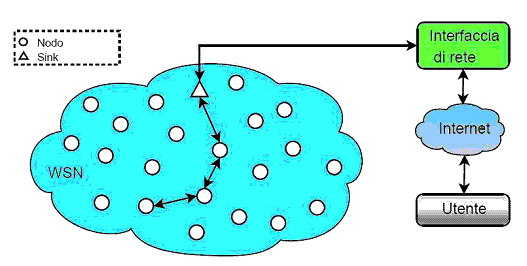
\includegraphics[width=0.95\textwidth,height=\textheight,keepaspectratio]{images/fig_1_1}
\caption{Rete WSN}
\label{fig:3_1}
\end{figure}
\newline
La comunicazione avviene in maniera asimmetrica, in quanto i nodi inviano i dati monitorati verso dei nodi speciali chiamati Sink, i quali sono gli unici nodi detta rete che si interfacciano con un calcolatore o un cloud. Le reti WSN devono avere diversi requisiti, fra i quali bassi consumi, scalabilit�, flessibilit� ed i nodi devono essere di piccole dimensioni ed a basso costo.
\subsection{Topologia di una WSN}
Le topologie di reti utilizzate in una WSN sono sostanzialmente tre:
\newline
- \textbf{Stella}: prevede un nodo centrale che funge da coordinatore della rete. Un qualsiasi altro nodo per comunicare con gli altri invia il messaggio al coordinatore che lo inoltra al destinatario; tutti i messaggi eseguono al massimo due hop. � la topologia pi� semplice che permette l'uso di protocolli e algoritmi altrettanto semplici.
\newline
- \textbf{Mesh}: nelle reti mesh o peer-to-peer ogni nodo della rete pu� comunicare con gli altri nodi della rete che rientrano nella sua copertura radio. I nodi sono considerati tutti uguali, perci� hanno tutti le stesse prestazioni. Viene definita \textit{multihop}, ovvero un messaggio pu� attraversare pi� nodi intermedi. I vantaggi sono che si possono creare reti pi� grandi e si possono avere percorsi ridondanti che aumentano affidabilit� e robustezza, introducendo per� algoritmi complessi.
\newline
- \textbf{Albero}: i nodi formano un albero. I messaggi partono da un nodo della rete e risalgono verso la radice, che raccoglie e dati e funge da coordinatore, ovvero il Sink. Il rischio pi� grande di questa topologia � proprio il sovraccarico del Sink.
\newline
\begin{figure}[htbp]
\centering
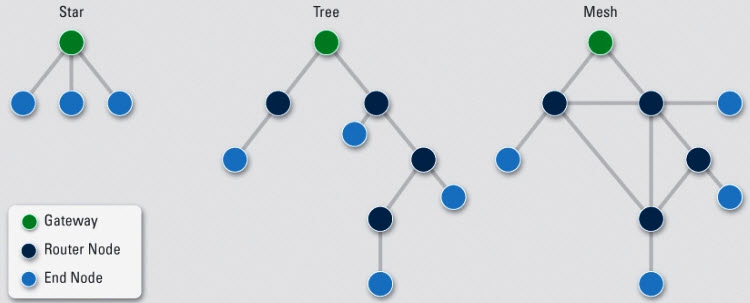
\includegraphics[width=0.95\textwidth,height=\textheight,keepaspectratio]{images/fig_1_2}
\caption{Topologie Rete WSN}
\label{fig:3_1}
\end{figure}
\newline

WSN ha un grandissimo potenziale ma ancora non ha raggiunto la sua efficacia ottimale. Ci� � dovuto alle sfide intrinseche presenti e la domanda crescente dalle applicazioni, il che ha portato ad aumentare l'interesse nella ricerca negli ultimi anni. Le maggiori sfide che dovr� affrontare WSN saranno sulla efficienza energetica, migliorare la comunicazione ed il routing.

\section{Software Defined Networking}
SDN � un paradigma il cui compito principale � quello di disaccoppiare le funzioni di controllo della rete da quelle di inoltro del traffico. Questo paradigma nasce proprio per risolvere i problemi delle reti tradizionali, ovvero la scarsa scalabilit� e complessit�, le quali non riuscivano a soddisfare le richieste di mercato dovute alla richiesta maggiore di applicazioni sempre pi� complesse ed un maggior numero di utilizzatori. 
\newline
Questo paradigma verr� abbondantemente trattato e definito in ogni sua sfaccettatura nei capitoli successivi. \cite{book}

\section{SDN-WISE}
SDN-WISE,� una soluzione Software Defined Network per Wireless Sensor Network. A differenza di SDN-WSN � stateful e propone due nuovi obbiettivi:
\newline
- riduzione di scambi di messaggi tra nodi e controller
\newline
- programmare i nodi come macchine a stati finiti cos� da poter abilitare operazioni che non potevano essere supportate da soluzioni stateless.
\subsection{Approccio SDN-WISE}
I Nodi di SDN-WISE sono racchiusi in tre strutture dati: WISE States Array, Accepted IDs Array e WISE Flow Table. Il Controller, come per l'approccio SDN, definisce le politiche di networking che verrano implementate dai vari sensori. In ogni momento i nodi SDN-WISE sono caratterizzati da uno stato corrente per ogni controller attivo. Il Wise States Array � una struttura dati che contiene il valore dello stato corrente.
\newline
In SDN-WISE, come nell'approccio SDN-WSN, � implementato il protocollo Sensor OverFlow (SOF) che permette ai nodi della rete di avere tabella di flusso (WISE Flow Table-WFT. Nel caso in cui un pacchetto venga processato, il sensore esplorer� le entries della WFT. Ciascuna entry of WFT contiene una sezione Matching Rules, nel quale vengono definite le condizioni per processare un pacchetto. In caso contrario il nodo richiede aiuto al controller. 
\newline
\newline
In SDN-WISE, la rete di sensori e i sink possono essere distinti. I Sink sono gateway tra il nodo sensore e il controller.
\newline
\begin{figure}[htbp]
\centering
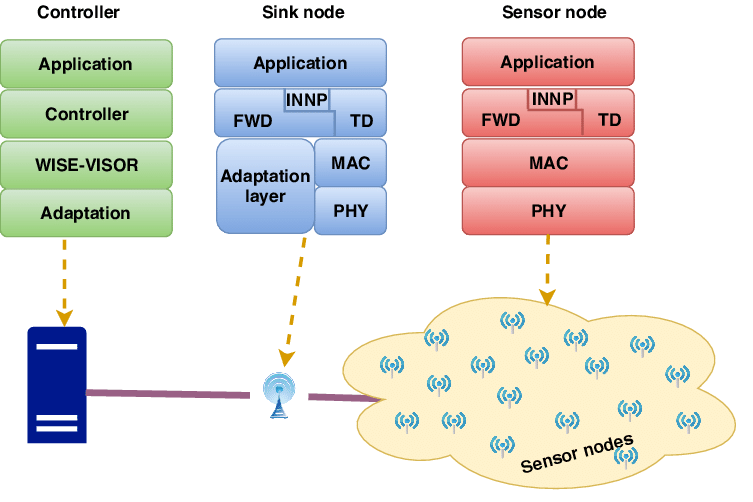
\includegraphics[width=0.95\textwidth,height=\textheight,keepaspectratio]{images/fig_1_3}
\caption{Architettura SDN-WISE}
\label{fig:3_1}
\end{figure}
\newline
I Pacchetti SDN-WISE hanno un header fissato, che consiste di 10 byte, divisi in vari campi come segue, figura:
\newline

\begin{figure}[htbp]
\centering
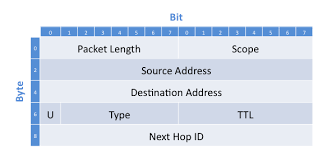
\includegraphics[width=0.95\textwidth,height=\textheight,keepaspectratio]{images/fig_1_4}
\caption{Header SDN-WISE}
\label{fig:3_1}
\end{figure}

- Il campo lunghezza del pacchetto contiene la lunghezza totale, incluso il payload, in bytes.
\newline
- Scope identifica un gruppo di Controller che hanno espresso interesse nel contenuto del pacchetto. Inizialmente � inizializzato a zero, ma pu� essere modificato attraverso appropriate entry della WFT.
\newline
- Indirizzo del Mittente e del Destinatario, come specificato nel nome, indicano gli indirizzi rispettivamente del nodo che ha generato il pacchetto e il nodo che lo riceve.












\chapter{Internet of Things}\label{ch:chapter2}

L'Internet of Things (IOT) � l'ultima tecnologia sviluppata nella lunga e continua rivoluzione nel mondo della comunicazione ed elaborazione dati. 
\newline
La sua dimensione ed influenza nella  vita di tutti i giorni, nel mondo del business e nel mondo politico ha schiacciato ogni tipo di tecnologia avanzata sviluppata in precedenza.

\section{Things of the Internet of Things}
Internet of Things (IOT) � un termine che si riferisce ai collegamenti in sviluppo che spaziano dai piccoli dispositivi smart fino agli applicativi con piccoli sensori. Il tema dominante � la possibilit� di mettere in comunicazione persone con oggetti ed oggetti con oggetti stessi. Attualmente l'internet che conosciamo oggi permette di interconnettere bilioni di industrie e di oggetti personali che usualmente si interfacciamo con sistemi Cloud. Invece l'IOT � principalmente guidato da dispositivi embedded. Questi dispositivi sono usualmente a bassa larghezza di banda, bassa ripetizione per l'acquisizione dati ed a bassa larghezza di banda per utilizzo dati che comunicano fra loro attraverso la user interface. 

\section{Evoluzione}
Le evoluzioni di Internet che hanno portato allo sviluppo dell'IOT sono quattro:
\newline
- INFORMATION TECHNOLOGY: PCs, servers, routers, firewalls e pi� in generale dispositivi IT con connessione internet.
\newline
- OPERATIONAL TECHNOLOGY (OT): macchine a applicativi non costruiti da compagnie IT, come ad esempio macchinari medici, SCADA(supervisory control and data acquisition) e processi di controllo.
\newline
- PERSONAL TECHNOLOGY: smartphones, tablets ed ebook reader, acquistati da vari clienti, che utilizzano connessione ad internet. Inoltre i dispositivi presentano varie forme di connettivit� wireless.
\newline
- SENSOR/ACTUATOR TECHNOLOGY: singoli dispositivi che utilizzano connettivit� wireless che fanno parte di grandi sistemi.

\section{Strati dell'Internet of Things}
La letteratura tecnica e quella business si focalizzano su due aspetti principali dell'IOT ovvero gli oggetti che sono collegati ad Internet che interconnette loro stessi.
\newline
La migliore visione dell'IOT � vederlo come un enorme sistema che consiste in cinque strati:
\newline
- Sensori e attuatori: questi sono oggetti. I sensori osservano l'ambiente e riportano delle misurazioni. Gli attuatori operano direttamente su quell'ambiente.
\newline
- Connectivity: un dispositivo pu� collegarsi via wireless o via cavo ad un network e mandare collezioni di dati al data center ( sensore) oppure ricevere comandi da un controllore (attuatori).
\newline
- Capacity: il network che supporta i dati deve essere capace di supportare un enorme flusso di dati.
\newline
- Storage: necessita di un largo storage per salvare e per mantenere i dati (backup). Generalmente avviene lato Cloud.
\newline
- Data Analytics: per un gran numero di dispositivi viene generato un flusso dati enorme che richiede di essere analizzato e processato.

\chapter{Requisiti e Tecnologie}\label{ch:chapter3}

Questo capitolo introduce due meccanismi che sono fondamentali nel flusso operativo del network e nella sua capacit� di trasmettere ed inviare pacchetti: il routing ed il congestion control.

\section{Routing}

\subsection{Caratteristiche}
La caratteristica principale di Internet � quella di ricevere pacchetti da una fonte ed inviarli ad una nuova destinazione. Per permettere questo � necessario che venga definita una strada attraverso la rete e generalmente vengono utilizzate le performance della rete come criterio di decisione. 
\newline
Il criterio pi� semplice che viene utilizzato il cammino minimo attraverso la rete, ovvero quello che passa attraverso il minor numero di nodi. � un criterio di misurazione molto semplice che permette di minimizzare le risorse utilizzare dalla rete. 
\newline
\begin{figure}[htbp]
\centering
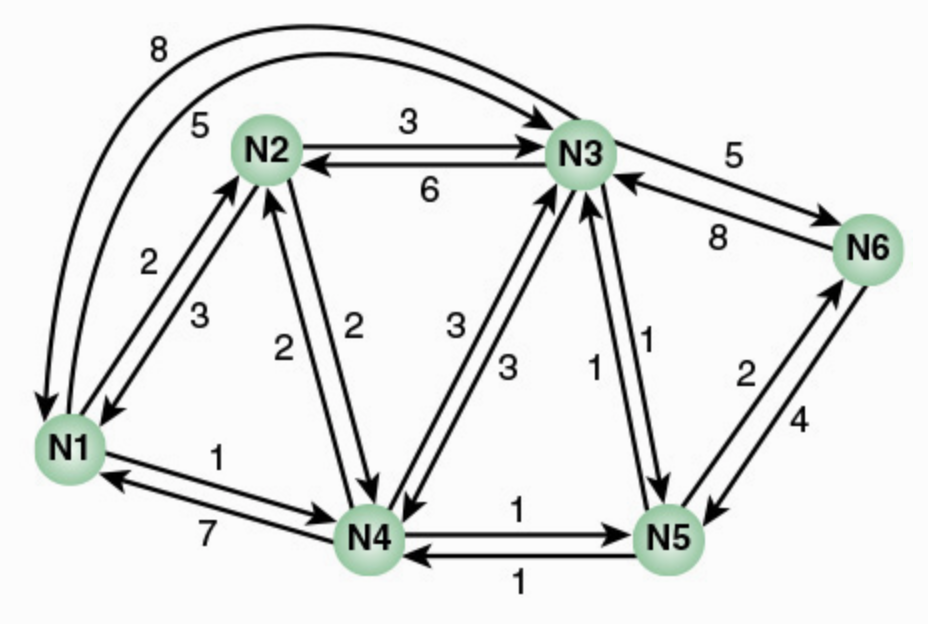
\includegraphics[width=0.80\textwidth,height=\textheight,keepaspectratio]{images/fig_2_7}
\caption{Esempio di architettura di rete}
\label{fig:3_1}
\end{figure}
\newline
Le politiche di routing vengono decise anche in base ad alcuni criteri, come ad esempio scegliere la strada pi� veloce, minimizzare il tempo di delay oppure si pu� decidere di adottare solo alcune strade sicure per politiche di sicurezza.

\subsection{Packet Forwarding - Inoltro Pacchetti}

La funzione chiave di ogni router � quella di accettare pacchetti in arrivo e reindirizzare quest'ultimi. Per favorire questo processo ogni router � dotato di forwarding tables, ovvero delle tavole di inoltro pacchetti che mostrano per ogni nodo le caratteristiche e le strade da percorrere per raggiungere il nodo successivo.
\newline
\begin{figure}[htbp]
\centering
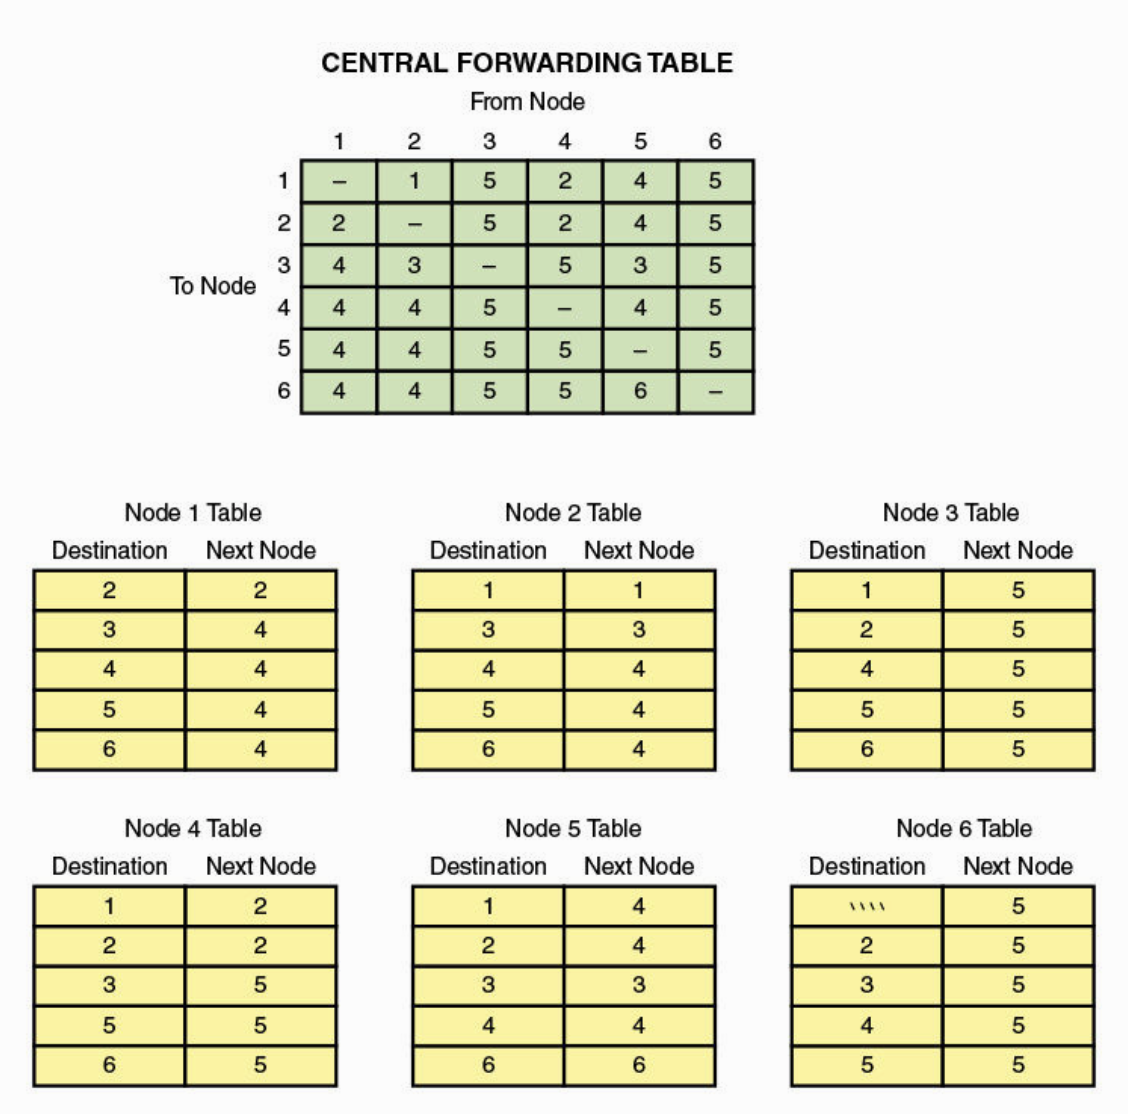
\includegraphics[width=0.50\textwidth,height=\textheight,keepaspectratio]{images/fig_2_8}
\caption{Packet Forwarding Tables}
\label{fig:3_2}
\end{figure}
\newline
Ogni router pu� essere responsabile di scoprire ed individuare le strade pi� appropriate oppure alternativamente pu� essere presente un network control center (centro di controllo della rete) che disegna le strade e mantiene una tabella di inoltro centrale. 
\newline
Le tabelle p� semplici, come quella mostrata in figura, contengono solo il nodo di destinazione, ma possono contenere anche informazioni addizionali come il source address, packet flow identifier ed il livello di sicurezza del pacchetto:
\newline
- FAILURE: quando un nodo o un collegamento fallisce non pu� pi� essere usato come parte della strada da seguire.
\newline
- CONGESTION: quando un'area della rete � fortemente congestionata, si desidera reindirizzare i pacchetti al di fuori dell'area della congestione, facendogli intraprendere strade alternative.
\newline
- TOPOLOGY CHANGE: l'inserimento di nuovi collegamenti o nodi modifica il routing (instradamento).

Per un sistema di routing adattivo, l'informazione sullo stato della rete pu� essere scambiata tra i nodi o tra i nodi e il central controller.

\subsection{Routing Protocols}
Ogni router � capace di prendere decisioni di instradamento dei pacchetti in base alla conoscenza e alla topologia della rete ed alle condizioni di traffico e delay di internet. 
\newline
Infatti tra i router � richiesto un accordo di cooperazione dinamica, in particolare i router devono evitare porzioni della rete che falliscono e devono evitare porzioni della rete dove ci pu� essere congestione. Per permettere questo tipo di decisioni i routers si basano su protocolli di routing. 
\newline
Esistono due categorie di protocolli di routing che sono basate sul concetto di autonomous system (AS). 
\newline
Un sistema AS richiede determinate caratteristiche:
\newline
1. Un AS � un set di router e di reti controllato da una singola organizzazione.
\newline
2. Un AS consiste in un gruppo di routers che si scambiano informazioni attraverso protocolli di routing.
\newline
3. Ad eccezione del tempo di fallimento, un AS � connesso (graph-theoretic sense); c'� una strada per ogni coppia di nodi.
\newline
Un protocollo routing, chiamato Interior Router Protocol (IRP) passa le informazioni fra router all'interno di un AS e non necessita di essere implementato all'estero del sistema. Questa flessibilit� permette agli IRPs di essere personalizzati su misura all'interno di specifiche applicazioni o per specifici requisiti. 
\newline
Pu� succedere che una rete sia costituita da pi� di un AS, come ad esempio una rete lan che collega pi� zone di un'universit�, che possono essere collegate per formare un unico AS. In questo caso gli algoritmi di routing e le tabelle di routing usate dai router possono cambiare. Infatti in questo caso al router devono essere passate anche informazioni esterne al singolo sistema AS e servir� un protocollo per passare informazioni attraverso routers di differenti AS. 
\newline
Questo protocollo prende il nome di exterior router protocol (ERP). Il protocollo ERP necessita di passare meno informazioni rispetto ad un IRP, poich� se ad esempio devo passare un'informazione fra due host di due reti AS, un router nel primo AS determina il target di AS ed indica una strada per raggiungere quel determinato sistema; una volta che il pacchetto � entrato in quel sistema, il router all'interno del sistema pu� cooperare per indirizzare quel pacchetto. 
\newline
L'ERP non conosce i dettagli e la strada che il pacchetto deve seguire una volta entrato nell'AS.

\subsection{Elementi del Router}

\begin{figure}[htbp]
\centering
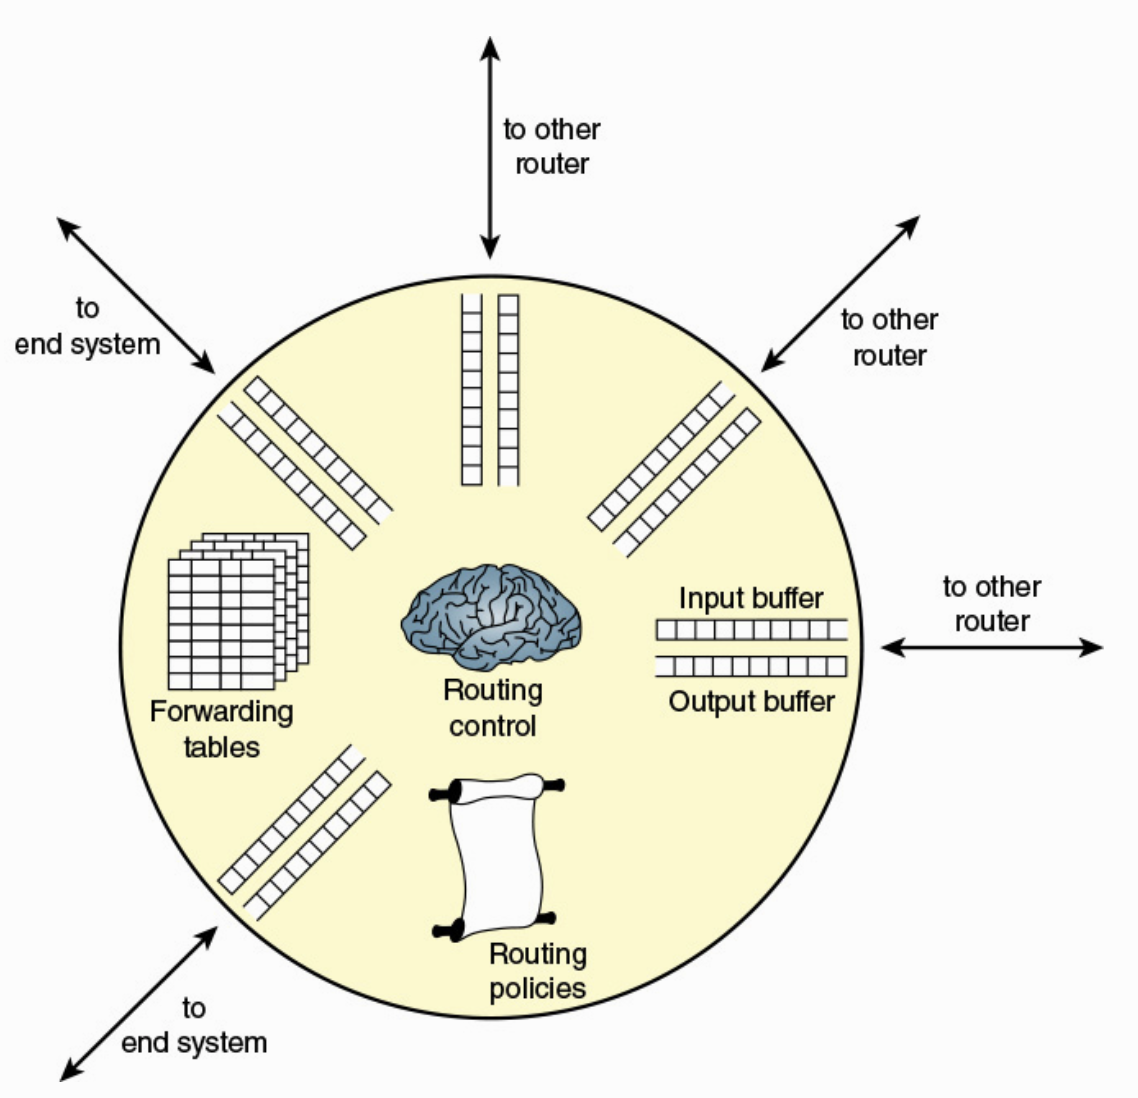
\includegraphics[width=0.60\textwidth,height=\textheight,keepaspectratio]{images/fig_2_10}
\caption{Elementi del router}
\label{fig:3_3}
\end{figure}
\
 La figura mostra una funzione di controllo del routing che include in particolare esecuzione di protocolli di routing, mantenimento di tabelle di routing e la supervisione alle politiche di controllo della congestione.
\newline
Ogni router � dotato di porte I/O connesse a quest'ultimo. Su ogni porta arrivano e partono pacchetti; per semplificare il modello possiamo dire che da una parte si accettano i pacchetti in arrivo e dall'altra si mantengono i pacchetti in attesa che partano. 
\newline
I pacchetti che arrivano sono memorizzati nell'input buffer della corrispondente porta, dopodich� il router lo esamina e prende una decisione basata sulle tabelle di inoltro dei pacchetti e sposta il pacchetto sul corrispondente output buffer. 
\newline
I pacchetti in coda per l'output sono trasmessi il pi� velocemente possibile e vengono messi in coda secondo la politica FIFO (First In First Out). Pi� comunemente ci sono anche altre regole pi� complesse che gestiscono questo flusso, come ad esempio la dimensione del pacchetto.

\section{SDN e NFV}
Con lo sviluppo e l'incremento del volume e della variet� del traffico internet, dovuto alla grande ricerca come i big-data, cloud computing e traffico mobile, � diventato sempre pi� difficile trovare un punto d'incontro tra QoS e requisiti QoE. Le reti hanno bisogno di essere pi� flessibili e adattive ed � per questo che si sono sviluppate due tecnologie adottate da diversi servizi network, ovvero il software-defined networking (SDN) e il network functions virtualization (NFV). \cite{sdn}

\subsection{Software Defined Networking}
L'SDN ha raggiunto un cos� ampio livello che sta rimpiazzando i tradizionali modelli network, infatti permette un enorme livello di flessibilit� e di personalizzazione che va incontro alle nuove esigenze di networking e alle esigenze di tutto il compartimento IT come ad esempio il cloud, la mobilit�, social network e video.
\newline
\newline
\textbf{FUNZIONALIT� DELL'SDN}
\newline
Ci sono due elementi che si prendono parte all'inoltro dei pacchetti, ovvero una funzione di controllo (control function) che decide la strada da seguire e la relaziona in base al traffico della rete, e una funzione dati (data function) che inoltra i dati basandosi sulle politiche della function control. Prima dell'avvento dell'SDN queste funzioni erano integrate nei dispositivi i connessi alla rete (router, bridge, packet switch). Con l'SDN, un controller centrale racchiude tutte le funzioni pi� complesse, incluso il routing, la nomenclatura, la policy e i controlli di sicurezza. 
\newline
\begin{figure}[htbp]
\centering
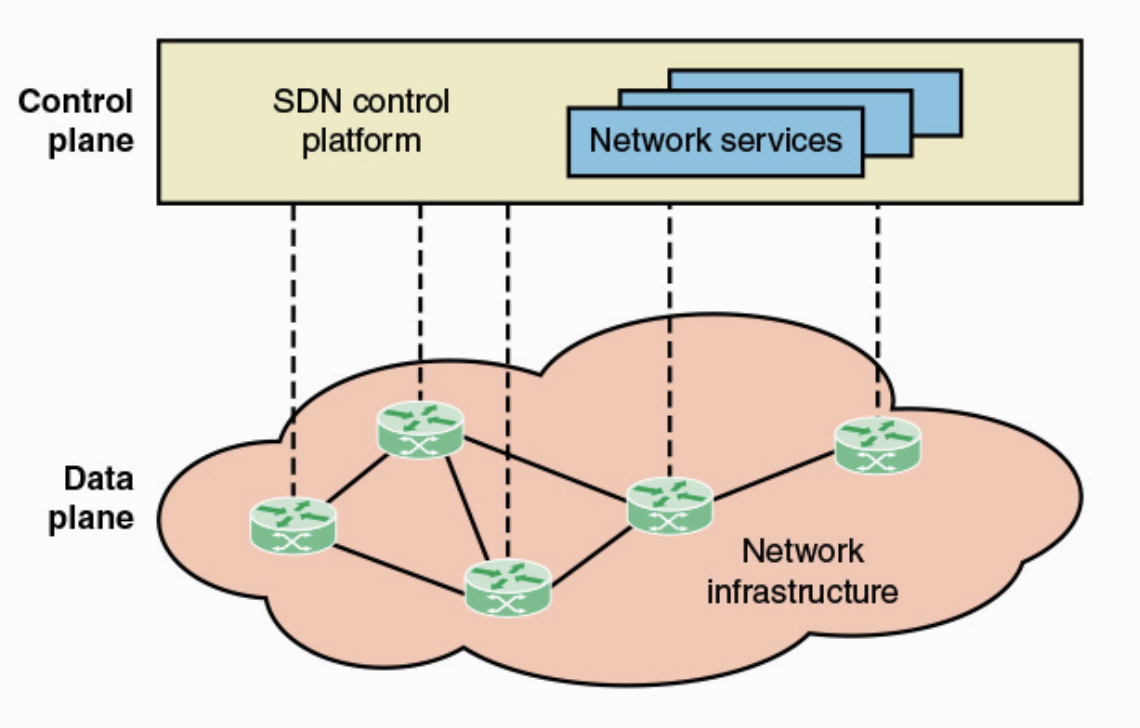
\includegraphics[width=0.80\textwidth,height=\textheight,keepaspectratio]{images/fig_2_15}
\caption{Software Defined Networking}
\label{fig:3_4}
\end{figure}\newline
Questo costituisce l'SDN control plane che � formato da uno o pi� SDN controller, i quali definiscono il flusso di dati che occorre nell'SDN data plane. Tutto il flusso attraverso la rete � configurato dal controller che verifica la fattibilit� della comunicazione attraverso le politiche della rete. Se il controllore accorda il flusso, calcola una strada che quest'ultimo deve seguire ed apre il flusso a tutti gli switch presenti sulla rete, i quali si occupano solo di controllare il flusso. Questi switches costituiscono il data plane. La comunicazione fra controller e switches usa protocolli standard. 
\newline
\newline
\textbf{KEY DRIVERS}
\newline
Un fattore chiave dell'SDN � la incredibile diffusione di server virtuali. Questi ultimi permettono di mascherare le risorse del server, il numero e le entit� che compongono il server, i processori, il sistema operativo e gli utenti. Questo � possibile partizionando una singola macchina in multipli ed individuali servers conservando le risorse hardware. Inoltre rende possibile la migrazione del server in caso di possibili fallimenti della rete. La virtualizzazione dei server � diventato un elemento centrale in combinazione con i big data ed il cloud computing, ma ha creato problemi con l'architettura rete tradizionale. Un problema � la configurazione delle virtual LAN, VLAN, che necessitano di essere riconfigurate ogni volta che viene spostato un server virtuale. Un altro effetto della virtualizzazione dei server � che il modello � molto diverso dal classico client/server a cui siamo abituati, poich� i server sono in continua comunicazione fra loro ed i flussi server-to-server cambiano di locazione ed intensit� tantissime volte, richiedendo un approccio flessibile al network. Un altro fattore che richiede una risposta rapida nell'allocare risorse network � la continua evoluzione ed il continuo aumento nell'utilizzo di dispositivi mobili, come smartphone, tablet e computer portatili che rapidamente cambiano il loro punto di connessione alla rete, la quale deve essere in grado di cambiare rapidamente le risorse, il QoS e mantenere la sicurezza sui dispositivi mobili.
L'infrastruttura network esistente � in grado di rispondere ai cambiamenti per il controllo del traffico, ma questo richiede una grande spesa di tempo e di infrastrutture se la rete � molto grande e ci sono molti dispositivi. La rete deve configurare ogni tipologia di dispositivo separatamente ed aggiustare le performance ed i parametri di sicurezza sessione per sessione e per tipo di applicazione. Su una larga scala, quando una macchina virtuale, VM, viene creata pu� richiedere ore o perfino giorni per essere configurata.

\subsection{Network Function Virtualization}
Attualmente la tecnologia delle VM attraverso internet o nell'industria del network � stata usata con la funzione di server a livello applicativo come ad esempio database servers, cloud server, web servers and email servers. La stessa tecnologia pu� essere per� utilizzata per i dispositivi della rete come ad esempio routers, LAN switches, firewall e IDS/IPS servers. 
Il Network Function Virtualization (NFV) scollega le funzioni della rete, come per esempio il routing, il firewalling, intrusion detection ed il Network Address Translation dalle piattaforme proprietarie hardware e implementa queste funzioni via software. Utilizza tecnologie virtuali standard che girano su dispositivi hardware molto performanti per virtualizzare queste funzioni del network ed � applicabile sia alle infrastrutture di rete via cavo che wireless. 
NFV ha un delle propriet� in comune con SDN:
- muove funzionalit� sul lato software
- usa piattaforme hardware dedicate invece di piattaforme hardware proprietarie
- usa applicazioni standard o applicazioni aperte (APIs)
- supporta con pi� efficienza modifiche e cambiamenti della rete
NFV ed SDN sono indipendenti ma complementari poich� quest'ultimo scollega i dati ed il piano di controllo, rendendo il controllo e l'instradamento della rete pi� flessibile ed efficiente. NFV invece scollega le funzioni della rete da specifiche piattaforme hardware attraverso la virtualizzazione per rendere queste funzioni p� flessibili ed efficienti. Anche SDN pu� essere virtualizzato, ma invece che usati singolarmente, SDN ed NFV possono essere combinati per raggiungere grandi benefici e grandi performance. 

\chapter{SDN: Background and Motivation}\label{ch:chapter4}
\section{Requisiti dell'Evoluzione Network}
Un incredibile numero di articoli sta invitando le aziende che sviluppano dispositivi network e gli utenti a rivalutare il concetto dell'approccio tradizionale all'architettura della rete. Questi articoli sono raggruppabili in incremento della domanda, fornitura ed i pattern del traffico.

\subsection{Incremento Della Domanda}
- Cloud Computing: c'� stato un enorme passaggio sia per i servizi pubblici che privati ai servizi cloud. 
\newline
- Big Data: processare enormi quantit� di data-set richiede l'utilizzo di migliaia di server in parallelo, che devono essere interconnessi gli uni con gli altri. C'� un'enorme e costante incremento di domanda per la capacit� delle reti network ed i data center.
\newline
- Mobile Traffic: gli impiegati accedono alla rete della loro azienda costantemente anche dall'esterno, con i loro smartphone, tablet e pc. Questi dispositivi hanno sofisticate app che generano traffico audio-video, aumentando continuamente il carico della rete.
\newline
- The Internet of Things (IOT): la maggior parte degli oggetti genera un traffico modesto, anche se ci sono delle eccezioni come le video camere di sorveglianza. Un grande numero di questi dispositivi pu� rappresentare per la rete dell'azienda un grosso carico.

\subsection{Fornitura in Aumento}
Con l'incremento della domanda per la rete, anche le tecnologie della rete per assorbire questo grande traffico sono in continuo aumento ed evoluzione, in particolare dopo che le reti 4G e 5G hanno dato la possibilit� ai dispositivi mobili di connettersi in massa alla rete. L'incremento delle tecnologie di trasmissione della rete � dovuto anche all'incremento dei vari dispositivi, come i LAN switches, routers, firewall, intrusion detection/prevention systems. Anno dopo anno stanno diventando sempre pi� grandi, con memorie pi� veloci, con buffer pi� grandi e ad accesso pi� rapido, tanto veloci quanto un processore. 

\subsection{Traffic Pattern molto complessi}
Con lo sviluppo di tutte queste tecnologie, si � sviluppato anche lo schema di traffico della rete e le architetture di rete tradizionali faticano a stare al passo con la domanda. Infatti fino ad oggi l'architettura dominante nelle imprese � il modello client-server che permette interazioni fra un client ed un server; in questo ambiente la rete pu� essere configurata staticamente ed � facilmente prevedibile il traffico della rete.
\newline
Un numero di sviluppatori ha mostrato quale potrebbe essere un modello pi� dinamico e con complessi schemi di traffico all'interno dell'industria:
\newline
- Gli applicativi client/server devono accedere a server e database multipli che devono comunicare fra loro, generando traffico orizzontale fra server e traffico verticale come il modello client/server.               
\newline
- La convergenza sulla rete di voce, dati, video genera un traffico impredicibile.
\newline
- Le UC (Unified Communications) hanno un pesante di applicazioni che necessitano un accesso multiplo ai servers.
\newline
- Il pesante uso di dispositivi mobili permette all'utente di accedere in ogni momento a dati e applicativi aziendale da ogni dispositivo e da ogni luogo. Infatti il traffico mobile � diventato una significante parte dell'infrastruttura di rete industriale.
\newline
- Il diffuso uso di cloud pubblici ha spostato quello che prima era il traffico locale per molte industrie, risultando in continuo aumento e con flussi di caricamento impredicibili.
\newline
- La nuova pratica comune di applicazioni e database server virtuali ha incrementato significativamente gli hosts che richiedono un alto volume di traffico per accedere alla rete e di conseguenza in ogni cambiamento fisico di dislocazione delle risorse del server.

\subsection{Le Architetture di Rete Tradizionali sono Inadeguate}
Con il grande sviluppo degli schemi di trasmissione e le crescenti performance dei dispositivi network, l'architettura di rete tradizionale risulta sempre pi� inadeguata. 
\newline
Il modello tradizionale di Internet si basa su un'architettura che utilizza il protocollo TCP/UDP, il quale ha tre caratteristiche portanti: 
\newline
- Sistema di indirizzamento finale a due livelli
\newline
- Routing basato sulla destinazione
\newline
- Sistema distribuito, controllo autonomo
\newline
Tradizionalmente il routing era  basato su ogni indirizzo di destinazione di ogni singolo pacchetto. In questo approccio di tipo DATAGRAM, dove ogni pacchetto � indipendente dal successivo, i pacchetti successivi possono seguire differenti strade attraverso internet ed i router si impegnano per trovare il cammino per ogni singolo pacchetto che comporti il minor ritardo. Pi� recentemente, per soddisfare i requisiti del QoS, i pacchetti vengono processati in termini di flussi di pacchetti.
\newline
L'ONF (Open Networking Foundation) ha delineato quattro limitazioni generali della tradizionale architettura di rete:
\newline
- Architettura statica e complessa: per rispondere alla  domanda di cos� tanti livelli di QoS, alto flusso di traffico e requisiti di sicurezza l'architettura � diventata sempre pi� complessa e difficile da gestire con un numero enorme di protocolli che aggiungono sempre pi� informazioni alla rete. La difficolt� pi� grande si ha quando si aggiungo o si muovono dispositivi all'interno della rete.
\newline
- Politiche inconsistenti: per implementare la sicurezza della rete su larga scala � necessario effettuare migliaia di modifiche. Infatti quando in una rete molto vasta si aggiunge una macchina virtuale (VM), quest'ultima pu� richiedere molte ore o addirittura giorni per essere configurata.
\newline
- Impossibile da ridimensionare: con l'aumento della domanda per la rete, sia in volume che in variet�, una soluzione adottabile potrebbe essere quella di aggiungere  switch e dispositivi di trasmissione, ma questo risulta complesso a causa della staticit� della rete. Allora si pu� pensare a sovrascrivere porzioni di sottorete basandosi sulla predicibilit� dei modelli di traffico, ma a causa dell'incremento dell'utilizzo della virtualizzazione e la variet� di applicazioni multimediali, tutto questo diventa impossbile.
\newline
- Dipendenza dal fornitore: per la natura attuale del traffico e della richiesta di rete, le imprese devono proporre e sviluppare nuove capacit� e servizi per rispondere al cambiamento del business e alla domanda degli utenti. Un cospicuo numero di open interface ha abbandonato il mondo delle imprese per la scarsa produttivit� dei fornitori.                               

\section{L'Approccio SDN}
In questo capitolo parleremo dell'SDN mostrando come � stato disegnato e progettato per rispondere ai requisiti che richiede l'evoluzione della rete.

\subsection{Requisiti}
La ODCA (Open Data Center Alliance) ha diramato una lista di requisiti per definire un approccio moderno alla rete:
\newline
- Adaptivit�: la rete deve  aggiustare e rispondere dinamicamente in base alla necessit� della singola applicazione, delle condizioni della rete o dell'esigenza di una azienda.
\newline
- Automazione: i cambiamenti delle policy devono essere diramati automaticamente, in modo tale da ridurre l'errore umano e il lavoro manuale.
\newline
- Manutenzione: l'introduzione di nuove caratteristiche e capacit� (update software, patches) deve avvenire senza interrompere la continuit� e senza causare interruzioni alle operazioni. 
\newline
- Modello di gestione: i software di gestione della rete devono permettere la gestione della rete a livello di modello, invece di implementare cambiamenti concettuali che necessitano di modificare singolarmente ogni elemento.
\newline
- Mobilit�: le funzioni di controllo devono soddisfare anche la mobilit�, inclusi dispositivi mobili degli utenti e server virtuali.
\newline
- Sicurezza integrata: le applicazioni di rete devono integrare senza interrompere la sicurezza, che deve essere ritenuta come uno dei servizi chiave e non come una aggiunta finale.
\newline
- Ridimensionamento su scala: l'implementazione deve avere la capacit� di adattare la rete e i suoi servizi in base alla richiesta. 

\subsection{Architettura SDN}
Una analogia che possiamo disegnare sull'evoluzione dell'architettura della rete � il paragone che nasce spontaneo con lo sviluppo verticale delle architetture dei computer e dei loro sistemi operativi. Infatti ad oggi tutto l'ambiente di sviluppo hardware e software � dotato di una grandissima flessibilit�; questo infatti permette ha permesso lo sviluppo di macchine virtuali che possono essere spostate da un server all'altro e attraverso piattaforme di diversa natura hardware e software. 
\newline

\begin{figure}[htbp]
\centering
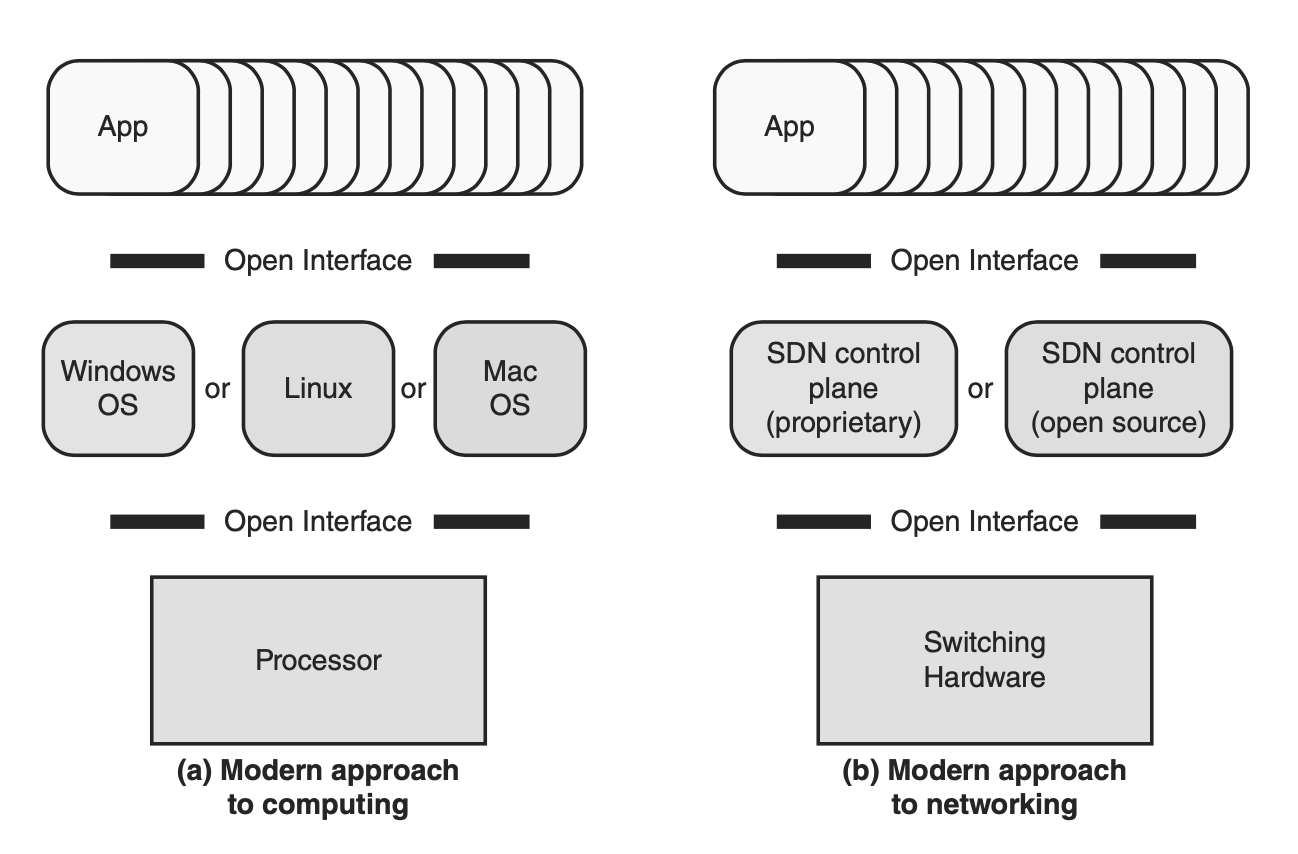
\includegraphics[width=0.80\textwidth,height=\textheight,keepaspectratio]{images/fig_3_1}
\caption{Approccio Moderno}
\label{fig:3_1}
\end{figure}

L'ambiente delle reti ad oggi si trova a dover fare i conti con alcune limitazioni e la difficolt� maggiore � quella di fare interfacciare le diverse applicazioni con l'infrastruttura della rete. 
\newline
Il concetto centrale dell'approccio SDN � quello di permettere agli sviluppatori e ai gestori delle reti di avere lo stesso tipo di controllo che ad oggi si ha sui server x86. Il concetto di open interface applicato all'architettura SDN � quello di avere differenti applicativi che comunicano nello stesso modo con i controller SDN.
\newline

\begin{figure}[htbp]
\centering
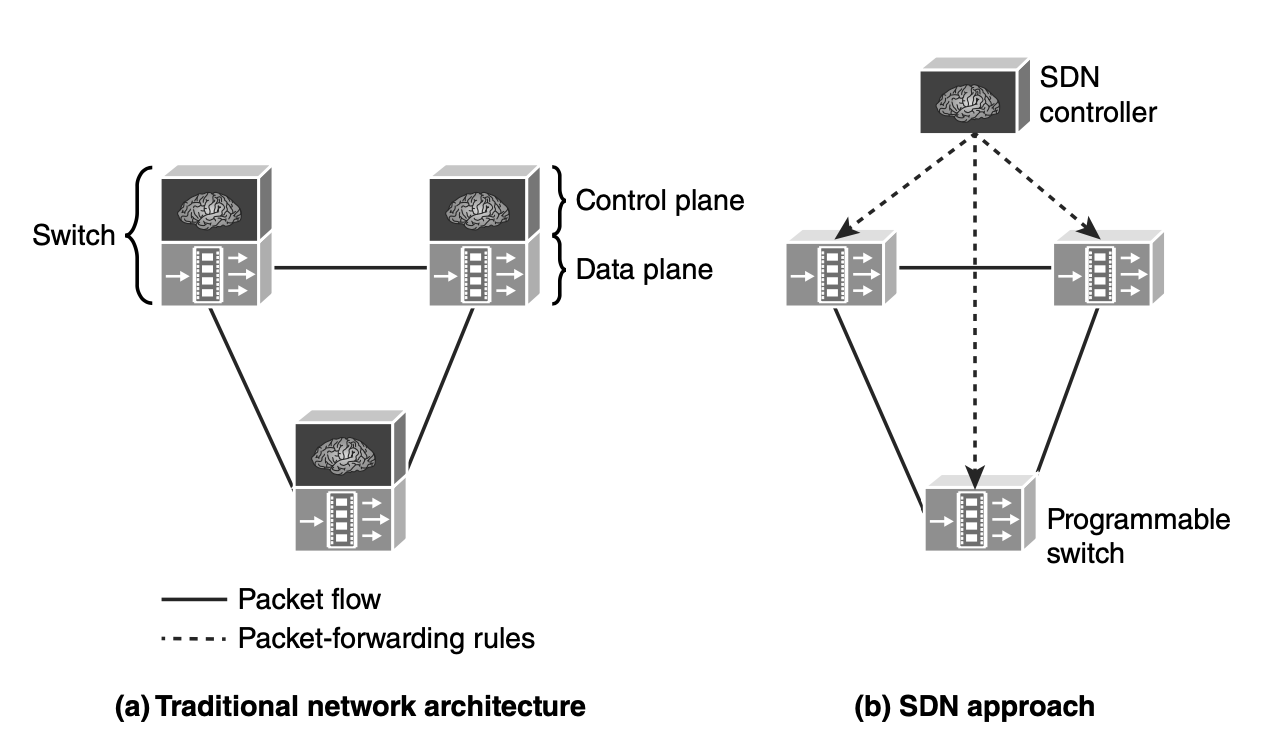
\includegraphics[width=0.90\textwidth,height=\textheight,keepaspectratio]{images/fig_3_2}
\caption{Control and Data Plane}
\label{fig:3_2}
\end{figure}

Il data plane consiste in vari switches fisici e switches virtuali. In entrambi i casi gli switches si occupano di inoltro dei pacchetti. Le altre caratteristiche interne come ad esempio buffer o priority parameters sono modellate in base alle richieste del cliente. Ogni switch deve implementare un modello, fisico o astratto, di inoltro pacchetti. Questo modello � definito in termini di un open application programming interface (API) tra il control plane e il data plane (southbound API). 

\begin{figure}[htbp]
\centering
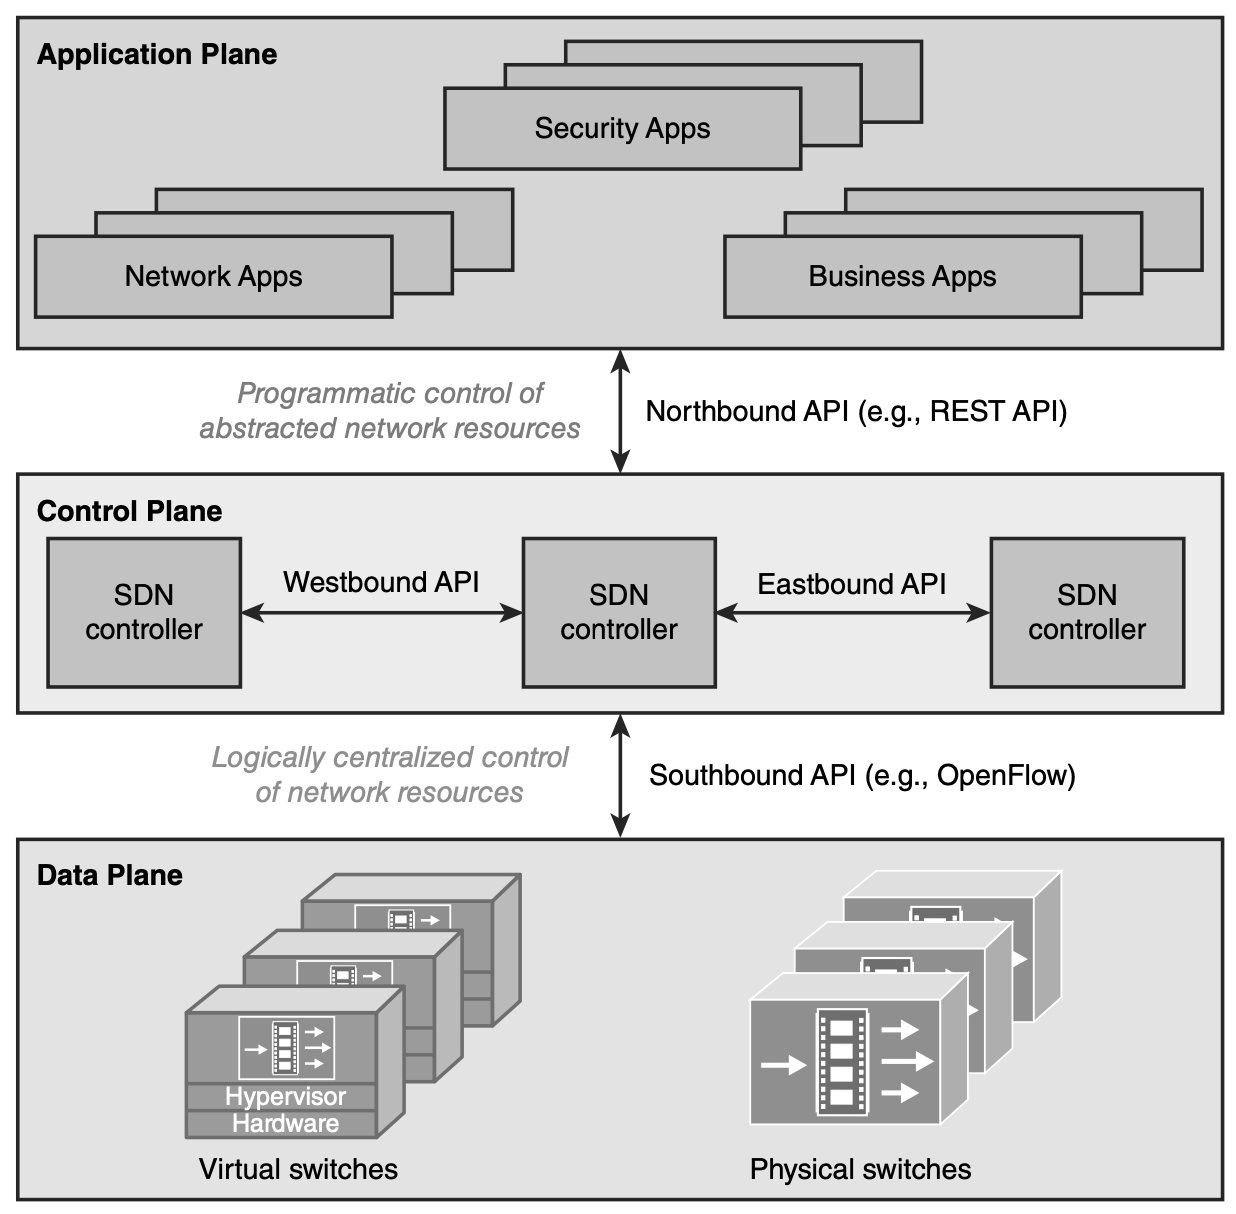
\includegraphics[width=0.80\textwidth,height=\textheight,keepaspectratio]{images/fig_3_3}
\caption{Architettura SDN}
\label{fig:3_3}
\end{figure}

I controller SDN possono essere implementati direttamente su un server o su un server virtuale. OpenFlow o altre open API sono utilizzate per controllare gli switch nel data plane. In addizione, i controller utilizzano le informazioni sulle capacit� e sulla domanda ottenuti dall'equipaggiamento della rete attraverso cui passa il flusso dei dati. I controller SDN mostrano inoltre le Northbound API che permettono agli sviluppatori e ai gestori delle reti di sviluppare un alto numero di applicativi personalizzati, molti dei quali non era possibile realizzare prima dell'avvento dell'SDN. 
\newline
Sono inoltre pensate delle horizontal APIs (Eastbound/Westbound) che sono capaci di comunicare e cooperare fra gruppi di controllers per sincronizzare gli stati.
\newline
A livello applicativo ci sono una variet� di applicazioni che possono interagire con i controller SDN. Un esempio sono reti ad alta efficenza energetica, monitoraggio di sicurezza, controllo degli accessi e gestione della rete.

\subsection{Caratteristiche dell'SDN}
Mettendo tutto insieme, le caratteristiche chiave dell'SDN sono le seguenti:
\newline
- Il control plane � separato dal data plane. I devices del data plane sono semplici dispositivi di inoltro pacchetti (packet-forwarding).
\newline
- Il control plane � implementato in un controller centralizzato. Il controller SDN ha quindi una visione centralizzata della rete o delle reti sotto il suo controllo. Il controller � un software portatile che pu� girare su server ed � capace di programmare l'inoltro dei dispositivi forte della sua visione centralizzata.
\newline
- Le open interfaces sono definite tra i dispositivi nel control plane e quelli nel data plane.
\newline
- La rete � programmabile in base alle applicazioni che girano in cima ai controller SDN. I controller SDN presentano una visione astratta delle risorse di rete per i vari applicativi.

\section{SDN- e NFV-Related Standard}
A differenza di altre aree tecnologiche, non c'� nessun corpo responsabile di sviluppare gli open standard per l'SDN o NFV. Piuttosto ci sono un alto numero di organizzazioni, consorzi industriali e svariate iniziative impegnate nel creare degli standard e delle linee guida per l'SDN e l'NFV. 

\subsection{Standard Developing Organizations}
Internet Society, ITU-T ed ETSI stanno avendo un contributo chiave nella standardizzazione dell'SDN e dell'NFV. 

\subsubsection{Internet Society}
I gruppi pi� attivi all'interno dell'Internet Society (ISOC) sono due: IETF e IRTF. L'ISOC � il comitato di coordinamento per il design, l'ingegnerizzazione e la gestione di Internet. Le aree coperte includono operazioni all'interno dello stesso Internet, standardizzazione di protocolli usati da sistemi o dalla rete Internet.
\newline
L'\textbf{Internet Engineering Task Forse (IETF)} ha gruppi di sviluppo che lavorano in aree specifiche dell'SDN:
\newline
- \textit{Interface to routing system (I2RS)}: sviluppa la capacit� di interagire con i router e i protocolli di routing da applicare alle politiche di routing.
\newline
- \textit{Service function chaining}: sviluppa l'architettura e le capacit� dei controllers di dirigere flussi di traffico attraverso la rete in modo tale che ogni piattaforma di servizio virtuale veda solo il traffico che deve dirigere.
\newline
L'\textbf{Internet Research Task Force (IRTF)} ha effettuato delle pubblicazioni che riguardano l'approccio nel costruire l'architettura dei layer SDN, discussioni in merito alle southbound API o alle varie APIs per i protocolli di routing.

\subsubsection{ITU-T}
La \textit{International Telecommunication Union-Telecommunication Standardization Sector (ITU-T)} � un'agenzia che ha definito standard nell'area delle telecomunicazioni. 
\newline
All'interno dell'ITU-T ci sono quattro team di studio (SGs):
\newline
- SG 13: network futuri, includendo il cloud computing, mobile e i network della next-generation.
\newline
- SG 11: requisiti di segnale, protocolli e test sulle specifiche.
\newline
- SG 15: trasporto, accessi e reti di casa.
\newline
- SG 16: multimedia.

\subsubsection{ETSI: European Telecommunications Standards Institute}
ETSI � riconosciuto dall'Unione Europea come una organizzazione europea standard anche se risulta un'organizzazione no-profit nonostante abbia un'impatto internazionale. Infatti ETSI ha avuto un ruolo chiave nel definire gli standard dell'NFV a livello di architettura, infrastruttura, metriche di qualit� del servizio e politiche di sicurezza.

\subsection{Industry Consortia}
I consorzi di definizione degli standard hanno iniziato a svilupparsi negli anni 80 con lo scopo di fornire gli standard all'interno dell'avanzata frenetica del mondo tecnologico.
\newline
Il consorzio pi� importante nel mondo dell'SDN � l'\textit{Open Networking Foundation (ONF)} che � interamente dedicato alla promozione e all'adozione dell'SDN attraverso standard di sviluppo aperti. Il pi� importante contributo � la realizzazione di un protocollo OpenFlow e la realizzazione di API.  
\newline
Il protocollo OpenFlow � la prima interfaccia standard disegnata per l'SDN ed � gi� stata impiegata nello sviluppo di diverse reti, sia a livello hardware che software. 

\subsection{Open Development Initiatives}
Ci sono una serie di iniziative aperte che lavorano generalmente alla realizzazione di standard pubblici o di open software. Il numero di questi gruppi � diventato sempre pi� attivo nello sviluppo dell'SDN e l'NFV.
\newline
\textbf{OpenDaylight}
\newline
OpenDaylight � un software open source realizzato per girare su Linux. I suoi membri hanno realizzato numerosi controller per un'ampia gamma di applicativi.
\newline
\textbf{Open Platform for NFV}
\newline
Open Platform for NFV � un progetto open source dedicato ad accelerare l'adozione degli standard dell'NFV, aumentarne la consistenza, le performance e le componenti open source.  
\newline
\textbf{OpenSlack}
\newline
OpenSlack � un software open source che ha l'obiettivo di realizzare un cloud operating system completamente open source. 

\chapter{SDN Data Plane and OpenFlow}\label{ch:chapter5}
\section{SDN Data Plane}
Con il termine SDN Data Plane spesso ci si riferisce al livello infrastrutturale ovvero il livello dopo i dispositivi connessi alla rete performano il trasporto e il processo dei dati in accordo con le decisioni prese dall'SDN Control Plane. 
\newline
La caratteristica chiave dei dispositivi connessi alla rete nell'SDN � che questi ultimi performano una semplice funzione di inoltro dei dati senza bisogno di software che prendano decisioni al loro posto. 

\subsection{Funzioni del Data Plane}
Le principali funzioni dei dispostivi network sono le seguenti:
\newline
- \textbf{Control Support Function}: interagisce con il livello di controllo dell'SDN per supportare la porgrammabilit� attraverso l'interfaccia di risorse e controllo. Gli switch comunicano con il controller comunica con gli switch attraverso il protocollo OpenFlow degli switch. 
\newline
- \textbf{Data Forwarding Function}: accetta i flussi di dati provenienti da altri dispositivi network per inoltrarli sulle strade che sono state predefinite in accordo con il livello applicativo dell'SDN. 
\newline
Queste regole di instradamento utilizzate dai dispositivi network sono rappresentate dalle tabelle di instradamento che indicano per determinate categorie di pacchetti qual'� il loro prossimo passo da fare all'interno della rete.

\subsection{Protocollo del Data Plane}
Il protocollo � supportato da tutti i dispositivi network. Il flusso dei pacchetti dati consiste nel flusso di pacchetti IP; pu� quindi essere necessario per le tabelle di instradamento definire le entrate nei campi ad alto livello dei pacchetti, come avviene nel TCP o nell'UDP. La rete esamina l'IP header ed altri possibili header in ogni pacchetto per prendere le decisioni di instradamento. d

\section{OpenFlow}
Per tradurre il concetto di SDN nella implementazione pratica devono verificarsi due condizioni:
\newline
- deve essere presente una architettura logica comune fra gli switch, i router e gli altri elementi della rete; inoltre il tutto deve essere controllato da un controller SDN.
\newline
- un protocollo standard e sicuro � necessario tra il controller SDN ed i dispositivi network.
\newline
Questi requisiti sono indirizzati dall'OpenFlow, il quale � sia un protocollo tra l'SDN ed i dispositivi della rete che una specifica logica degli switch facenti parte della rete. Ogni switch � infatti in grado di connettersi agli \textbf{OpenFlow switches} e possibilmente il tutto si connette direttamente ai dispositivi finali che sono fonti o destinazione del flusso di pacchetti. Dalla parte degli switch l'interfaccia � nota come \textbf{OpenFlow Channel} e queste connessioni avvengono tramite le Open Flow ports che servono anche per connettere gli switch al controller SDN.
\newline
OpenFlow ridefinisce tre tipi di porte:
\newline
- \textbf{Pyhsical Port}: corrispondono all'interfaccia hardware degli switch
\newline
- \textbf{Logical Port}: queste porte non corrispondono direttamente a qualche componente hardware degli switch. Le porte logiche sono infatti delle astrazioni che possono essere definite negli switch utilizzando dei metodi non-OpenFlow (link, tunnel, loopback interface). Possono includere l'incapsulamento dei pacchetti e possono mappare varie porte fisiche. � necessario che interagiscano con il processo OpenFlow cos� come fanno le porte fisiche.
\newline
- \textbf{Reserved Port}: definite da specifiche OpenFlow. Specificano regole generiche di instradamento come l'invio e la ricezione dal controller o l'inoltro utilizzando metodi non-OpenFlow, come fanno gli switch normali.
\newline
\newline
Le specifiche OpenFlow definiscono tre tipi di tabelle bell'architettura logica degli switch:
\newline
- \textbf{flow table}: abbinano pacchetti in ricezione ad un particolare flusso e specificano quale tipo di funzione deve processare i pacchetti. Ci possono essere pi� tabelle di flusso che operano nella pipeline.
\newline
- \textbf{group table}: le flow table possono dirigere il flusso alle group table che possono intraprendere una variet� di azioni che va ad inficiare uno o pi� flussi di pacchetti.
\newline
- \textbf{meter table}: � in grado di innescare una moltitudine di azioni in un flusso di pacchetti. 
\newline
\subsection{Flow Table Structure}
Il blocco principale dell'architettura logica degli switch sono le flow table. Ogni pacchetto che entra in uno switch passa attraverso una o pi� flow tables. Ogni flow table � formata da un  numbero di righe, chiamate \textbf{entries}, formata da sette componenti come si evince dalla figura.

\begin{figure}[htbp]
\centering
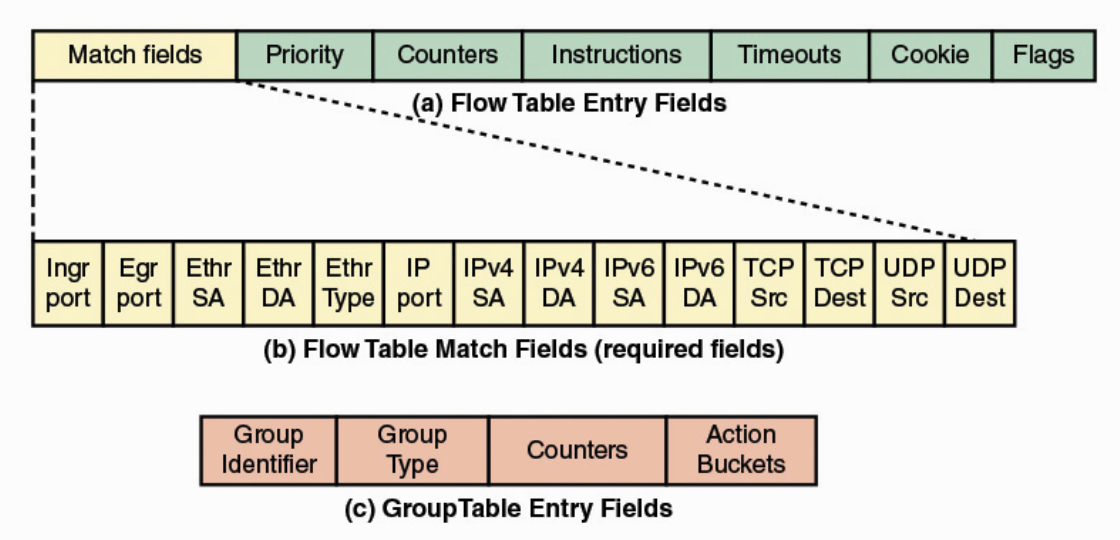
\includegraphics[width=0.95\textwidth,height=\textheight,keepaspectratio]{images/fig_4_5}
\caption{OpenFlow Table Entry Format}
\label{fig:4.5}
\end{figure}

\subsection{Flow Table Pipeline}
Uno switch include uno o pi� flow tables. Se � presente pi� di una flow table, quest'ultime sono organizzate come una pipeline, con le tabelle organizzate con numeri crescenti a partire da zero.
\newline
L'uso di tabelle multiple in una pipeline invece di una singola flow table aggiunge al controller SDN una notevole flessibilit�. 
\newline
L'OpenFlow specifica due stati di processing:
\newline
- \textbf{Ingress processing}: questo stato accade ogni volta, a cominciare dalla Tabella 0 ed utilizza l'identit� della porta di input. La Tabella 0 pu� essere anche l'unica ed in quel caso il processo � semplificato al processo di quella singola tabella e non c'� egress processing.
\newline
- \textbf{Egress processing}: � il processo che inizia dopo aver determinato la porta di output. Questo stato � opzionale ma se occorre coinvolge una o pi� tabelle. La separazione dei due stati � indicata dall'identificatore numero della prima egress table. Tutte le tabelle che hanno un numero inferiore della prima egress devono essere usate come ingress table e vicevera nessuna tabella con un numero maggiore o uguale della prima egress table pu� essere usato come ingress table.
\newline

\subsection{Group Table}
Nel corso del processo della pipeline una flow table pu� dirigere il flusso di pacchetti ad una group table o ad un'altra flow table. Le group table o le group actions abilitano l'OpenFlow a rappresentare un set di porte come una singola entit� per l'inoltro dei pacchetti. 
\newline
Differenti tipi di gruppi sono a disposizione per rappresentare differenti astrazioni di inoltro pacchetti, come il broadcasting ed il multicasting.
\newline
\newline
Ogni group table � costituita da un numero di righe, chiamate group entries, formata da quattro componenti:
\newline
- \textbf{Group Identifier}: un intero a 32 bit senza segno che unicamente identifica il gruppo. Un gruppo � definito come una entry della group table.
\newline
- \textbf{Group Type}: per determinare la semantica del gruppo.
\newline
- \textbf{Counters}: aggiornato quando i pacchetti sono processati da un gruppo.
\newline
- \textbf{Action bucket}: una lista ordinata di action bucket dove ognuna di queste contiene un set di azioni da eseguire e parametri associati. 

\section{Protocollo OpenFlow}
Il protocollo OpenFlow descrive lo scambio di messaggi che prende luogo tra l'OpenFlow Controller e l'OpenFlow Switch. Tipicamente il protocollo � implementato all'inizio del TLS per favorire un canale OpenFlow sicuro.
\newline
Il protocollo OpenFlow abilita il controller ad eseguire le azioni di add, update e delete al flusso il ingresso alla flow table. Quest'ultimo supporta tre tipi di messaggi: 
\newline
- \textbf{Controller to Switch}: questi messaggi iniziano dal controller ed in qualche caso richiedono una risposta dagli switch. Questa classe di messaggi abilita il controller a controllare lo stato logico dello switch, inclusa la sua configurazione ed i dettagli del flusso e degli ingressi nelle group table. Questo messaggio � inviato dal controller ad uno switch quando quello switch invia un pacchetto al controller ed il controller decide di non scartare il pacchetto ma di reindirizzarlo alla porta di output dello switch.
\newline
- \textbf{Asincrono}: questi tipi di messaggi sono inviati senza la sollecitazione del controller. Questa classe include vari messaggi di stato al controller. Include il messaggio di Packet-in, che pu� essere utilizzato dallo switch per inviare un pacchetto al controller quando non c'� nessun match sulla flow table.
\newline
- \textbf{Simmetrico}: questi messaggi sono inviati senza sollecitazioni ne da parte del controller ne dello switch. Sono semplici ed utili. Messaggi di "Hello" sono tipicamente inviati avanti e indietro fra il controller e lo switch quando la connessione viene stabilita. Questi messaggi di invio-risposta possono essere utilizzati sia dal controller che dallo switch per misurare la latenza, la banda, la interconnessione o per verificare che il dispositivo � online e funzionante.







\chapter{SDN Control Plane}\label{ch:chapter6}
\section{SDN Control Plane Architecture}
L'SDN control layer mappa le richieste dell'application layer in specifici comandi e direttive per il Data Plane. Il control layer viene implementato come un server o un set di server noti come SDN controllers. \cite{fog}
\subsection{Funzioni del Control Plane}
Le funzionalit� in dotazione all'SDN Controller posso essere viste come quelle di un \textbf{network operating sistem (NOS)}. Come su un convenzionale sistema operativo, un NOS ha in dotazione servizi essenziali, comuni interfacce applicative (APIs) e astrazioni di elementi di basso livello per gli sviluppatori. 
\newline
La funzione di un SDN NOS permette agli sviluppatori di definire politiche per la rete e controllare la rete senza preoccuparsi delle caratteristiche dei dispositivi che possono essere sia eterogenee che dinamiche. 
\newline
Un cospicuo numero di iniziative, sia commerciali che open source, ha portato all'implementazione di diversi SDN Controllers: OpenDaylight, Open Network operating System (ONOS), POX, Beacon, Floodlight, Ryu ed Onix.

\begin{figure}[htbp]
\centering
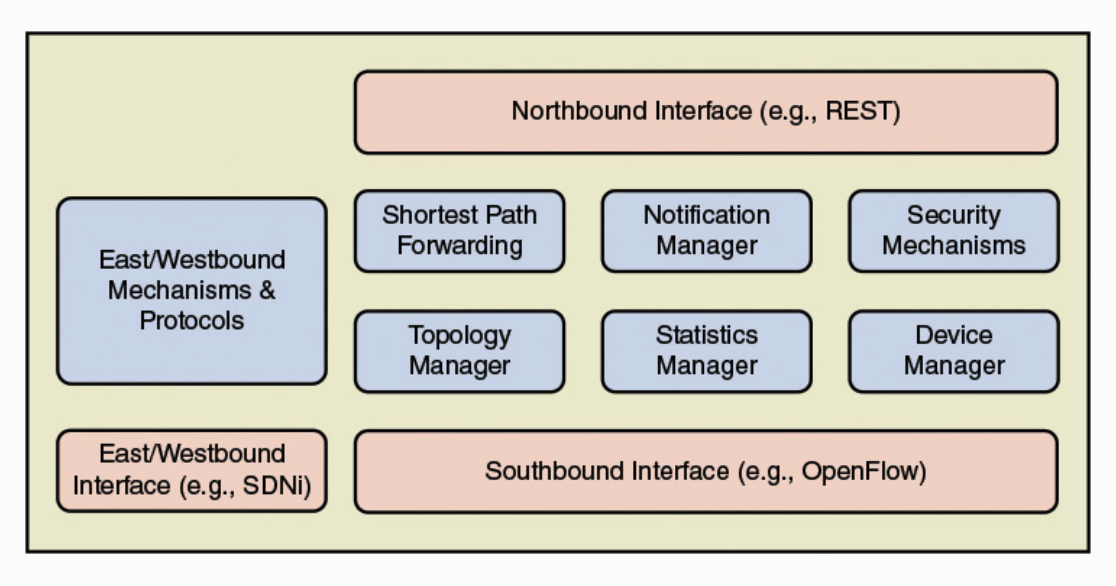
\includegraphics[width=0.60\textwidth,height=\textheight,keepaspectratio]{images/fig_5_2}
\caption{SDN Control Plane Functions and Interfaces}
\label{fig:5_2}
\end{figure}

\subsection{Southbound Interface}
La southbound interface si occupa della connessione logica tra il Controller SDN e gli switch del data plane. Alcuni controller supportano e consento di configurare solo un singolo southbound protocol. Un approccio pi� flessibile � l'uso di un southbound abstraction layer che permette una comune interfaccia per le funzioni del control plane e il supporto a molteplici APIs southbound.
\newline
L'implementazione pi� comune del southbound API � OpenFlow come abbiamo visto in precedenza.

\subsection{NorthBound Interfaces}

L'interfaccia northbound permette alle applicazioni di accedere alle funzioni del control plane e i vari servizi senza la necessit� di conoscere i dettagli dei sottostanti switch network. L'interfaccia northbound � tipicamente vista come una API software rispetto ad un vero e proprio protocollo. 
\newline
A differenza con la southbound interface non c'� nessuno standard da seguire o da rispettare. Il risultato di ci� � che sono state sviluppate innumerevoli controller complicando lo sviluppo delle applicazioni SDN. Per ovviare questo problema la Open Networking Foundation a costituito un Interface Working Group (NBI-WG) nel 2013 con l'obiettivo di definire e standardizzare un numero cospicuo di Northbound APIs. Attualmente non � stato ancora rilasciato nessuno standard. 

\begin{figure}[htbp]
\centering
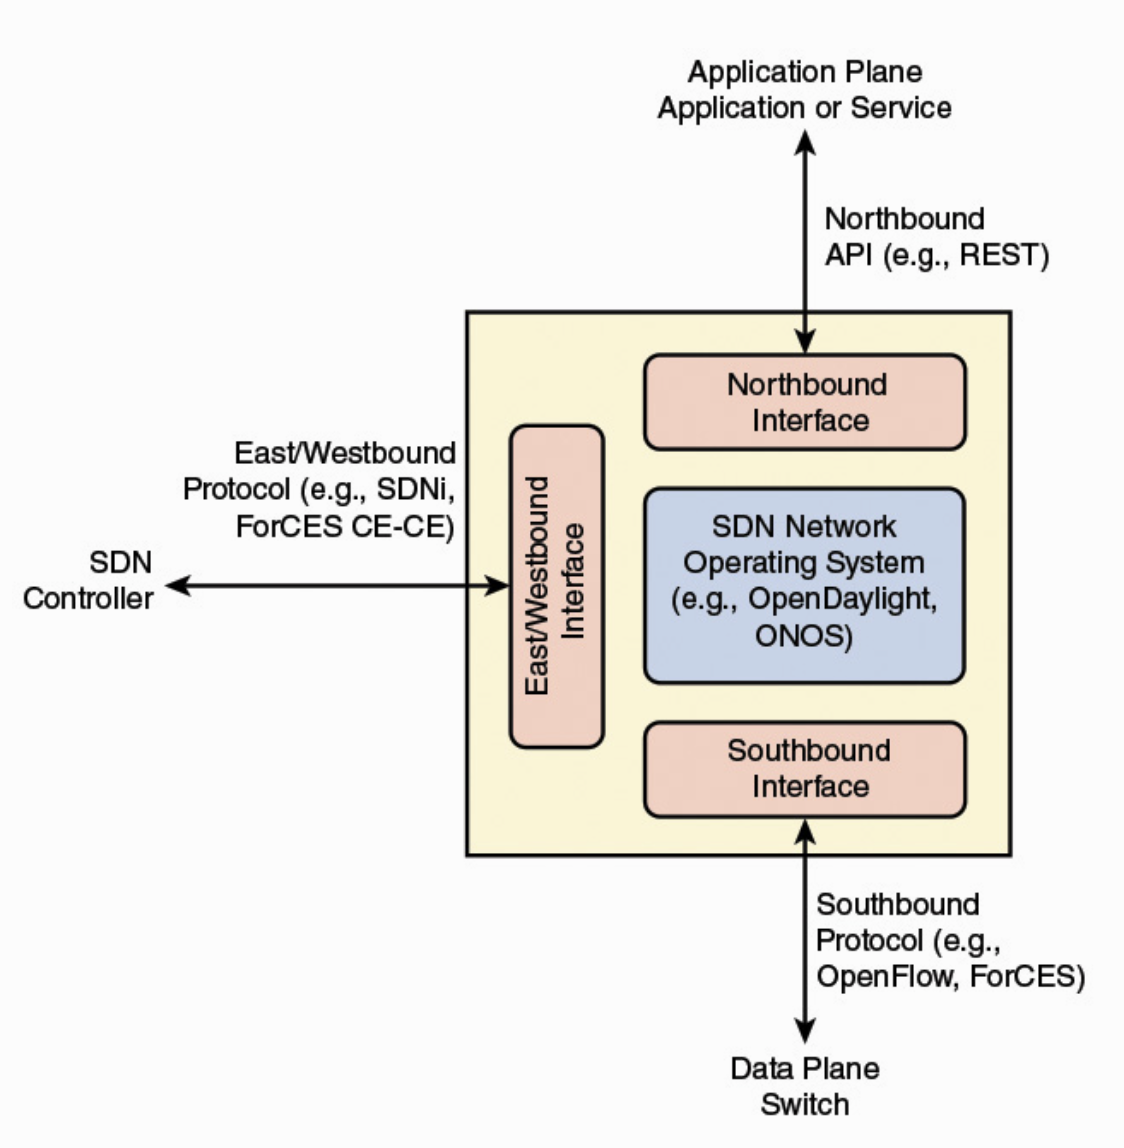
\includegraphics[width=0.60\textwidth,height=\textheight,keepaspectratio]{images/fig_5_3}
\caption{SDN Controller Interfaces}
\label{fig:5_2}
\end{figure}

\subsection{Routing}
Il network SDN richiede delle funzioni di routing. In termini generali le funzioni di routing includono una collezione di informazioni sulla topologia e sul traffico della rete ed un algoritmo per delineare al meglio i percorsi all'interno della rete.
\newline
Esistono due categorie di protocolli di routing:
\newline
- \textbf{Interior Router Protocols (IRPs)}: opera all'interno di sistemi autonomi (AS). I protocolli di routing pi� diffusi sono Open Shortest Path First (OSPF) Protocol e Enhanced Interior Gateway Routing Protocol (EIGRP).
\newline
- \textbf{Exterior Router Protocols (ERPs)}: opera attraverso sistemi autonomi. L'ERP � tipicamente eseguito solamente nei nodi a margine ed il protocollo di routing pi� utilizzato � il Border Gateway Protocol (BGP).
\newline
\newline
Tradizionalmente le varie funzioni di routing sono distribuite all'interno dei router che si trovano nella rete. Tuttavia, in una rete SDN-controlled, ha pi� senso centralizzare le funzioni di routing nel controller SDN poich� il controller pu� sviluppare una vista della rete pi� consistente ed aiutare a calcolare cammini pi� brevi all'interno della rete oltre ad aiutare l'implementazione delle applicazioni tenendo conto delle politiche di routing.
\newline
\newline
L'applicazione centralizzata del routing rappresenta due distinte funzioni:
\newline
- \textbf{Link Discovery}: le funzioni di routing devo essere a conoscenza dei link attraverso gli switches nel data plane. Nelle reti tradizionali il link attraverso i network avviene in maniera diretta come nel caso degli Ethernet switches. In addizione il link discovery deve essere realizzato attraverso un router ed un sistema di host e attraverso il router nel dominio del suo controller e il router nel dominio adiacente. 
\newline
- \textbf{Topology Manager}: mantiene la topologia di informazione per la rete e calcoler� le strade attraverso la rete. Il calcolo della rete determina il cammino pi� corto tra due nodi nel data plane o tra un nodo del data plane e un host.

\section{ITU-T Model}
In questo paragrafo descriveremo l'architettura SDN ad alto livello definita in ITU-T Y.3300.
\newline
L'\textbf{application layer} � dove le applicazioni SDN specificano servizi network o applicazioni business definendo le risorse della rete o i servizi fondamentali per loro. Le applicazioni interagiscono con l'SDN control layer attraverso le APIs che formano l'interfaccia application-control.

\begin{figure}[htbp]
\centering
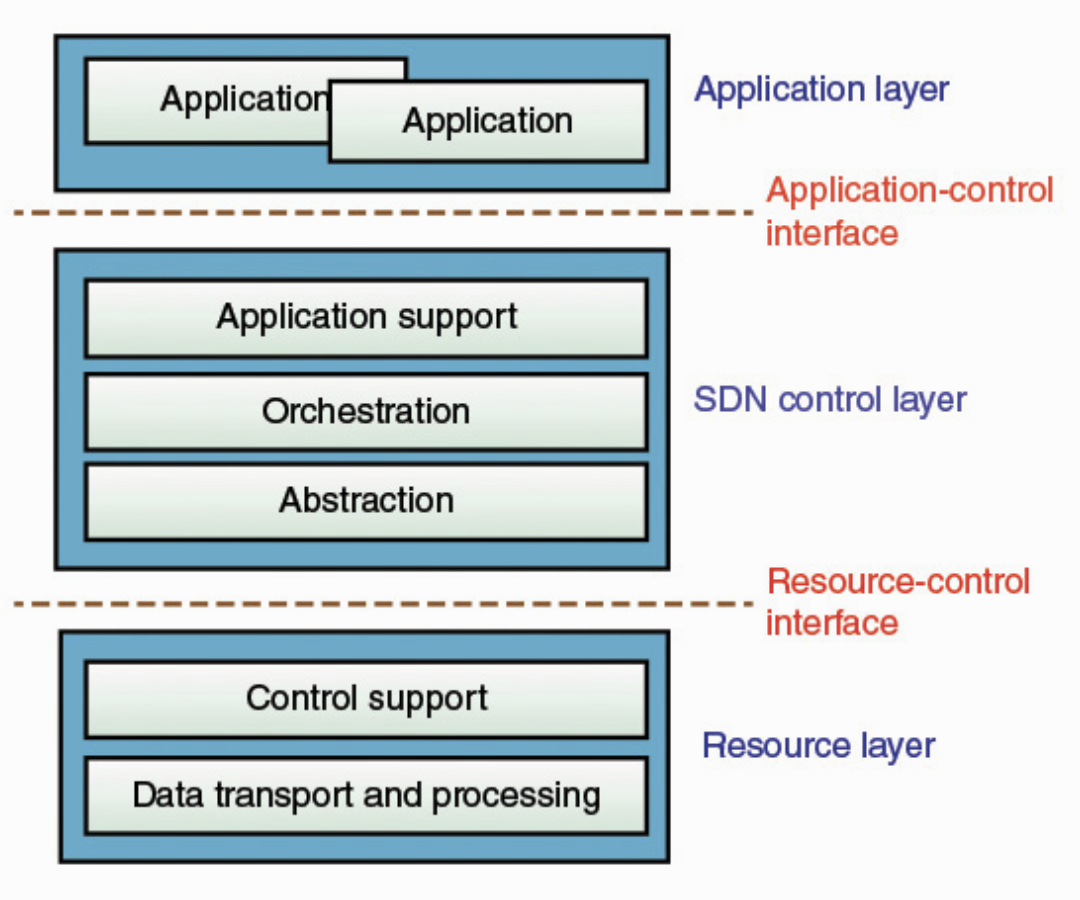
\includegraphics[width=0.60\textwidth,height=\textheight,keepaspectratio]{images/fig_5_6}
\caption{High Level Architecture of SDN(ITU-T Y.3300)}
\label{fig:5_6}
\end{figure}

Il \textbf{control layer} racchiude un significato di controllo  del comportamento delle risorse della rete. Il control layer pu� essere visto come i seguenti sublayers:
\newline
- \textbf{Application support}: fornisce un'API per le applicazioni SDN per accedere alle informazioni della rete e programmare specifici comportamenti della rete.
\newline
- \textbf{Orchestration}: fornisce il controllo automatico e la gestione delle risorse della rete; inoltre coordina le richieste dall'application layer verso le risorse della rete. Orchestration racchiude topologie di rete sia fisiche che virtuali, elementi della rete, controllo del traffico e altri aspetti correlati alla rete.
\newline
- \textbf{Abstraction}: interagisce con le risorse della rete e consente un'astrazione delle risorse della rete in tutte le sue caratteristiche a supporto del management e dell'orchestration della rete.
\newline
Il \textbf{resource layer} consiste nell'interconnessione degli elementi di instradamento del data plane, gli switches. Collettivamente questi ultimi consentono di trasportare e di processare i pacchetti di dati in accordo con l'SDN control layer. La maggior parte di questi controlli avviene per conto delle applicazioni. Il resource layer pu� essere visto come i seguenti sublayers:
\newline
- \textbf{Control support}: supporta la programmabilit� delle funzioni del resource-layer attraverso l'interfaccia del resource control.
\newline
- \textbf{Data transport and processing}: permette l'inoltro dei dati e le funzioni di routing.

\section{Rest}
\textbf{REpresentational State Transfer (REST)} � uno stile di architettura utilizzato per definire le APIs. � diventato lo stile di riferimento per le NorthBound APIs per i controller SDN. Una "REST API", o una API che si dice "RESTful" (ovvero che aderisce ai vincoli di REST) non � un protocollo, linguaggio o uno standard prestabilito ma rappresenta essenzialmente sei regole che le API devono obbligatoriamente seguire per definirsi RESTful.
\newline
\newline
\textbf{REST CONSTRAINTS}:
\newline
- \textbf{Client-server}: separazione fra interfaccia utente e dati salvati.
\newline
- \textbf{Stateless}: il server non memorizza nessun record dell'utente.
\newline
- \textbf{Cache}: ogni dato deve avere un'etichetta in cui � scritto se � "cacheable" oppure no. Nel caso in cui lo sia questa potr� essere riutilizzata in seguito.
\newline
- \textbf{Uniform interface}: REST enfatizza un'interfaccia uniforme tra i vari componenti. Per far questo REST definisce quattro regole:
\newline
1. Le risorse sono identificate mediante un identifier, ad esempio un URI.
\newline
2. Le risorse sono rappresentate in formati come JSON, XML, HTML.
\newline
3. Ogni messaggio ha abbastanza informazioni per descrivere come viene processato.
\newline
4. Un client non deve essere a conoscenza di come interagisce con il server.
\newline
- \textbf{Layered system}: una funzione � organizzata in livelli ed ogni livello comunica direttamente con il livello sotto o il livello sopra.
 \newline
- \textbf{Code on demand}: consente al cliente di essere scaricato per aumentare l'estensibilit� del codice.

\subsection{Esempio di REST API}
Consideriamo la funzione che descrive tutte le entit� di una group table di un particolare switch. L'URI di questa funzione � il seguente:
\newline
\textit{/stats/group/<dpid>} 
\newline
dove stats (statistiche) si riferisce al set di APIs che ricevono e aggiornano le statistiche e i parametri degli switch, mentre <dpid> (Data Path ID) � l'identificatore univoco per lo switch. Per invocare la funzione per lo switch 1 � necessario il seguente comando allo switch manager attraverso la REST API:
\newline
\textit{GET http://localhost:8080/stats/groupdesc/1} 
\newline
IL \textbf{localhost} indica che l'applicazione sta girando sullo stesso server. Nel caso in cui fosse stata remota l'URI sarebbe stato un URL che riesce ad accedere via HTTP attraverso il web.

\section{Cooperazione e coordinazione fra Controllers}
In addizione alle northbound e southbound interfaces, un tipico controller SDN ha una east/westbound interface che gli consente di comunicare con altri controller ed altre reti. Attualmente non ci sono stati significanti progressi su protocolli open source o protocolli standardizzati per le est/westbound interfaces.

\subsection{Controller Centralizzati vs Controller Distribuiti}
Un controller centralizzato � un singolo server che controlla tutto il data plane degli switches all'interno della rete.
\newline
Nelle grandi infrastrutture di rete, l'utilizzo di un solo controller che gestisce tutti i dispositivi network della rete risulta scomodo e indesiderato. Uno scenario pi� gradito sarebbe che venisse divisa la rete in un numero domini SDN non sovrapposti, chiamati anche \textit{SDN Islands} (figura 5.4) gestite da controller distribuiti.

\begin{figure}[htbp]
\centering
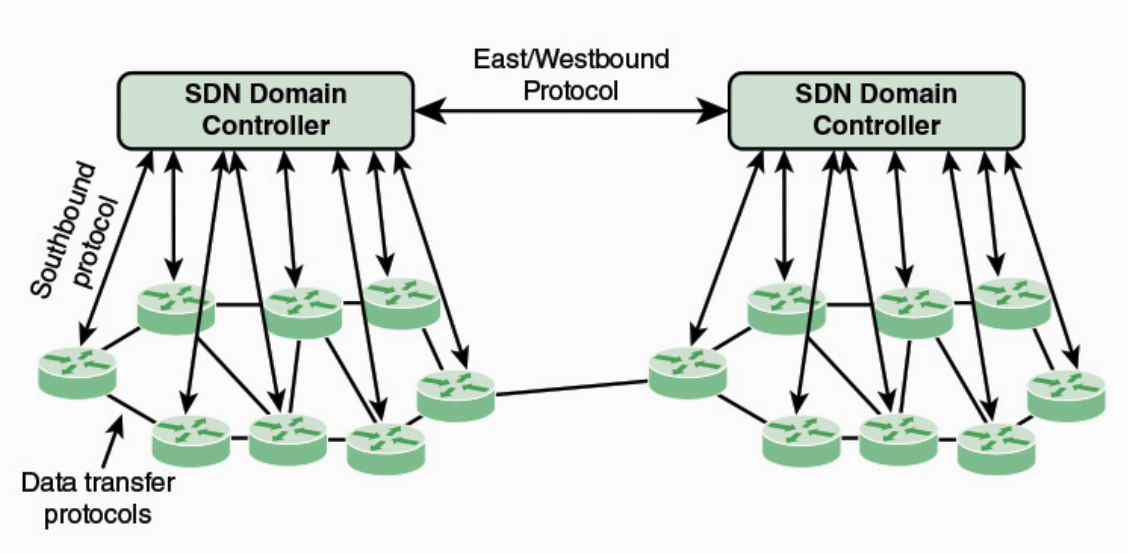
\includegraphics[width=0.80\textwidth,height=\textheight,keepaspectratio]{images/fig_5_7}
\caption{Struttura Dominio SDN}
\label{fig:5_7}
\end{figure}

Le ragioni per utilizzare i domini SDN sono le seguenti:
\newline
- \textbf{Scalability}: il numero di devices che un controller SDN pu� fisicamente gestire � limitato e proprio per questo motivo una rete molto grande ha bisogno di utilizzare pi� controller SDN.
\newline
- \textbf{Reliability}: l'uso di controllers multipli evita il rischio di avere un singolo punto di errore.
\newline
- \textbf{Privacy}: un operatore pu� scegliere di implementare differenti politiche di privacy in differenti domini SDN.
\newline
- \textbf{Incremental Deployment}: un operatore di rete pu� essere costituito da porzioni di infrastrutture datate e non. Dividendo la rete in dominio SDN multipli controllabili permette di ottenere flessibilit� nell'utilizzo e per gli sviluppi futuri.
\newline
\newline
I controller distribuiti possono essere collocati in piccole aree, in aree molto vasta oppure in una combinazione di esse. Controllers installati ravvicinati offrono un'alta produttivit� e sono appropriati per i data centers; invece controllers installati lontano possono contenere reti multilocation.
\newline
Tipicamente i controller distribuiti sono installati orizzontalmente ed in un'architettura distribuita � necessario un protocollo per permettere ai controller di comunicare.
 
\subsection{Border Gateway Protocol}
Il Border Gateway Protocol (BGP) � stato sviluppato per usare in congiunzione con i protocolli TCP/IP di Internet ed � diventato l'\textbf{exterior router protocol (ERP)} predefinito per Internet. 
\newline
BGP abilita i router, comunica con i gateways ed in differenti sistemi autonomi permettendo loro di comunicare e di scambiare informazioni di routing. Il protocollo opera attraverso dei messaggi che sono inviati attraverso connessioni TCP.
\newline
Ci sono tre funzionalit� coinvolte nel BGP:
\newline
- \textbf{Neighbor acquisition}: il termine \textbf{neighbor} indica che due router condividono la stessa rete. La neighbor acquisition avviene quando due router in due sistemi autonomi differenti concordano di scambiarsi informazioni regolarmente.
\newline
- \textbf{Neighbor reachability}: viene utilizzata per mantenere la relazione. Ogni partner deve essere sicuro che l'altra parte continua ad esistere e fa ancora parte della relazione stabilita in precedenza dai router. Per far ci� i router periodicamente si scambiano dei messaggi di \textit{Keepalive}.
\newline
- \textbf{Network reachability}: ogni router mantiene un database delle reti che pu� raggiungere e la strada preferita per raggiungere ogni rete. Quando viene modificato qualcosa nel database il router invia un messaggio di \textit{Update} agli altri routers.

\chapter{The Internet of Things: Components}\label{ch:chapter7}
\section{L'inizio dell'era IOT}
L'Internet del futuro coinvolger� un vastissimo numero di oggetti che useranno uno standard di architettura comune per portare determinati servizi agli utenti. Si prevede infatti che ci saranno decine di miliardi di questi dispositivi interconnessi fra loro nei prossimi anni e questo produrr� nuove interazioni fra il mondo fisico e quello digitale. La risultante di questo paradigma della rete prende il nome di \textit{Internet of Things (IOT} e produrr� un grandissimo numero di opportunit� per gli utenti, per le imprese e per chi fornisce servizi in svariati settori. In particolare le aree che beneficeranno maggiormente dello sviluppo dell'IOT saranno la collezione e l'analisi dei dati, automazioni, incluse nel settore del benessere e del fitness, automazioni per il controllo della casa, per risparmiare energia, per la produzione, per il trasporto, per il controllo ambientale, per lo stoccaggio e la produzione di prodotti, sicurezza e sorveglianza e molto, molto altro ancora.
\newline
Lo sviluppo tecnologico � ancora necessario in molte aree. Infatti negli ultimi anni sono stati condotti molti investimenti in ricerca e sviluppo delle reti wireless. Attualmente la ricerca e lo sviluppo di ricercatori e produttori � indirizzato su protocolli a basso consumo energetico, sicurezza e privacy, protocolli di rete ad alta efficenza energetica per una lunga durata della batteria, affidabilit� delle reti e nodi. Questi sviluppi wireless sono cruciali per la crescita dell'IoT.
\newline
Ci sono altre aree in cui � stato coinvolto lo sviluppo dei devices IoT come ad esempio la capacit� di social networking da parte dei dispositivi, sfruttando comunicazioni \textit{machine-to-machine}, processando e salvando un vastissimo numero di dati in real-time e sviluppando applicazioni che fornissero agli utenti finali interfacce utili e intelligenti per questi dispositivi e dati.

\section{Gli Scopi dell'Internet of Things}
Possiamo fornire le seguenti definizioni per definire gli scopi dell'IoT:
\newline
- \textbf{Internet of Things}: un'infrastruttura globale per le informazioni della societ�, che abilita servizi avanzati grazie all'interconnessione (fisica e virtuale) degli oggetti basandosi su tecnologie e informazioni attualmente esistenti ed in via di sviluppo.
\newline
- \textbf{Thing}: questo � un oggetto del mondo fisico o virtuale capace di essere identificato ed integrato all'interno di reti di comunicazione.
\newline
- \textbf{Device}: � una parte dell'IoT con la capacit� obbligatoria di comunicare e la capacit� opzionale di fare sensing, acuation, salvataggio dei dati e lavorazione di dati.
\newline
\newline

\begin{figure}[htbp]
\centering
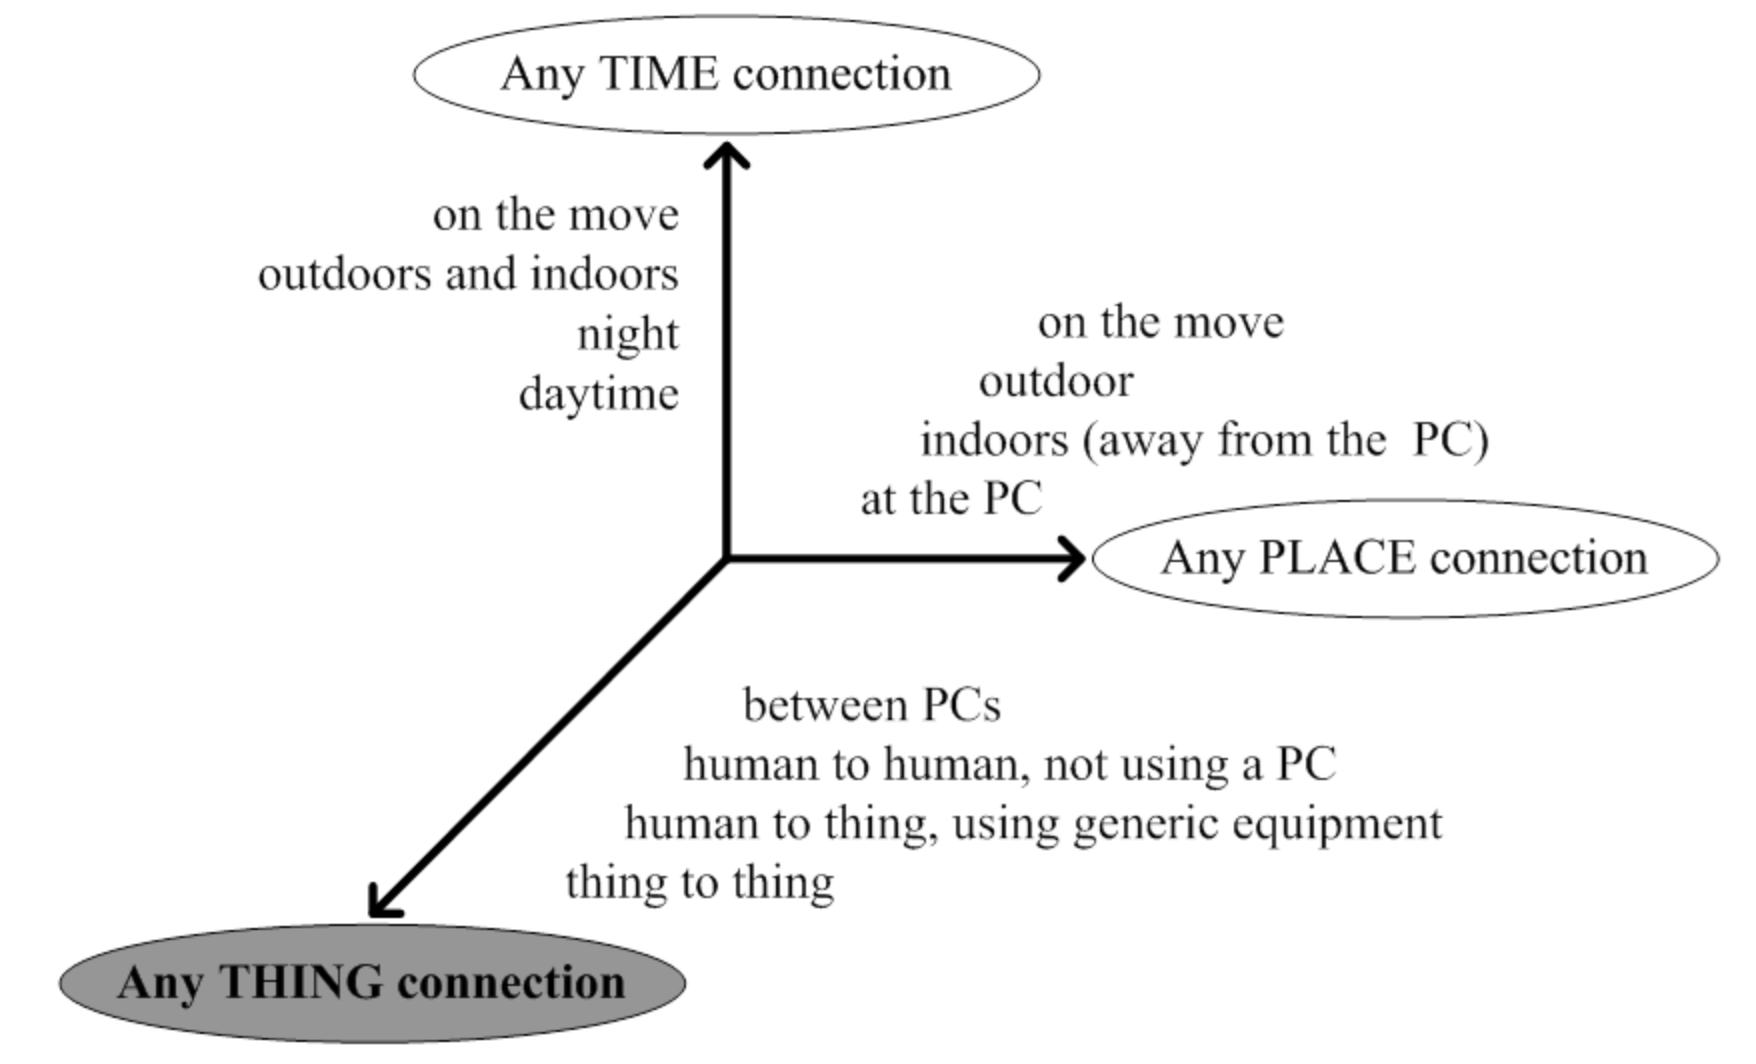
\includegraphics[width=0.80\textwidth,height=\textheight,keepaspectratio]{images/fig_5_8}
\caption{La nuova dimensione introdotta nell'Internet of Things}
\label{fig:5_7}
\end{figure}

L'equazione che pu� riassumere tutto il complesso sistema dell'IoT potrebbe essere la seguente:
\newline
\textit{Oggetti Fisici + Controller, Sensori, Attuatori + Internet} = \textbf{IoT}.

\section{Componenti di oggetti abilitati per l'IoT}
Gli ingredienti chiavi per un sistema di oggetti abilitati all'IoR sono sensori, attuatori, microcontrollers, un mezzo di comunicazione (transceiver) ed un mezzo di identificazione (RFID: radio-frequency identification). Il mezzo di comunicazione � un ingrediente fondamentale senza il quale i dispositivi non potrebbero partecipare in una rete. \cite{machine}

\subsection{Sensori}
Un sensore misura determinati parametri fisici, chimici o biologici e invia un segnale elettronico proporzionato con le caratteristiche rilevate, o in formato digitale oppure sotto forma di un livello di tensione analogico. In entrambi i casi, l'output del sensore � tipicamente l'input di un microcontroller o di un altro elemento di gestione.
\newline
Un sensore pu� operare in \textit{modalit� attiva} quando prende l'iniziativa di inviare i dati rilevati al controller o periodicamente o quando una determinata soglia � superata. Alternativamente il sensore pu� operare in \textit{modalit� passiva} inviando dati solo quando � richiesto dal controller.

\begin{figure}[htbp]
\centering
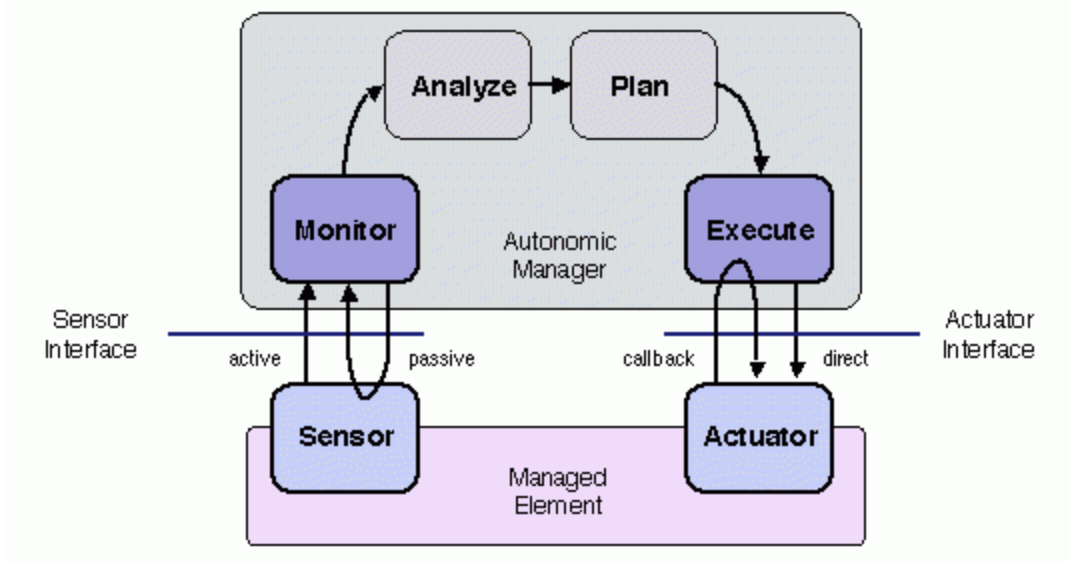
\includegraphics[width=0.80\textwidth,height=\textheight,keepaspectratio]{images/fig_5_9}
\caption{Interfacce per sensori e attuatori}
\label{fig:5_9}
\end{figure}

La tipologie di sensori utilizzati nell'IoT sono moltissime. Ci sono sensori che sono estremamente piccoli, usando nanotecnologie, oppure sensori estremamente grandi come camere di videosorveglianza.
\newline
\newline
Ci sono due concetti chiavi nel distinguere le tipologie di sonsori:
\newline
- \textbf{Accuracy}: si riferisce a quanto una misurazione si avvicina alla verit�. 
\newline
- \textbf{Precision}: si riferisce a quanto sono vicine tra loro pi� misurazioni della stessa quantit� fisica. Collegata con questo concetto troviamo la \textbf{Resolution}, ovvero la qualit� dell'output del sensore.
\newline
Se un sensore ha bassa accuracy, questo produce un errore sistematico. Se un sensore ha bassa precucione, produce un errore di riproducibilit�.

\subsection{Attuatori}
Un attuatore riceve un segnale elettronico dal controller e risponde interagendo con l'ambiente per produrre un effetto su qualche parametro fisico, biologico o chimico di una determinata entit�. 
\newline
Nella modalit� di operazione \textit{direct mode}, il controller invia un segnale che attiva gli attuatori. Invece nella \textit{callback mode} gli attuatori rispondono al controller per riportare un completamento o un problema e richiedono ulteriori istruzioni. 
\newline
\newline
Gli attuatori sono generalmenti classificati come segue:
\newline
- \textbf{Idraulici}: sono costituiti da un cilindro o un motore fluido che utilizza la forza idraulica per facilitare processi meccanici.
\newline
- \textbf{Pneumatici}: lavorano come quelli idraulici solo che utilizzano gas al posto di liquido.
\newline
- \textbf{Elettrici}: sono dispositivi alimentati da motori che convertono l'energia elettrica in coppia meccanica. 
\newline
- \textbf{Meccanici}: funzionano mediante movimento rotazionale o lineare e sono utilizzati per convertire il movimento. 

\subsection{Microcontrollers}
La cosa smart nei dispositivi che si definisco tali � fornita da un microprocessore perfettamente integrato. Adesso vedremo alcuni termini chiave per esplicare il concetto di microcontroller.
\newline
\textbf{Embedded System}
\newline
Il termine \textit{embedded system} si riferisce all'uso di elettronica e di software all'interno di un dispositivo che ha una o pi� funzioni.
\newline
\textbf{Application Processors vs Dedicated Processor}
\newline
\textit{Application processor} sono definiti dall'abilit� del processore di eseguire complessi sistemi operativi. Un classico esempio dell'uso di embedded application processor � lo smartphone, poich� � designato ad usare svariate applicazioni e svolgere molte funzioni diverse.
\newline
La maggior parte degli embedded systems utilizza un \textit{dedicated processor}, il quale � dedicato ad una o ad un piccolo numero di specifiche funzionalit� richieste dall'host. 
\newline
\textbf{Microprocessors}
\newline
Un processore i cui elementi sono stati miniaturizzati in un unico o in pi� circuiti integrati.
\newline
\textbf{Microcontrollers}
\newline
Un singolo chip che contiene il processore, la memoria non volatile (ROM), la memoria volatile per input/output (RAM), un clock ed una unit� di controllo I/O. Il loro impiego � fondamentale per utilizzare in maniera sostanzialmente differente lo spazio logico sul disponibile. 
\newline
\textbf{Deeply Embedded System}
\newline
� un sottoinsieme degli embedded system e possiamo dire che ha un processore il cui comportamento � difficile da osservare sia da parte del programmatore che dall'utente. Un deeply embedded system utilizza un microcontrollor, non � programmabile una volta che la logica del programma per il dispositivo � stata scritta nella ROM e non ha nessuna interazione con l'utente.

\subsection{Transceivers}
Un transceiver contiene i componenti elettronici necessari per ricevere e trasmettere dati. La maggior parte dei dispositivi IoT contiene un transceiver wireless, capace di comunicare utilizzando la Wi-Fi, ZigBee ed altri schemi wireless. 

\subsection{RFID}
La tecnologia Radio-frequency identification (RFID) utilizza onde radio per identificare oggetti e sta diventando una tecnologia che facilita sempre di pi� l'IoT.
\newline
Gli elementi principali per un sistema RFID sono i \textit{tags} ed i \textit{readers}. 
\newline
I \textit{tags} sono piccoli oggetti programmabili usati per il monitoraggio di oggetti, animali ed esseri umani. Sono disponibili in varie forme, dimensioni, funzionalit� e costi. 
\newline
I \textit{readers} acquisiscono e qualche volta riscrivono le informazioni salvate sui tags che rientrano nel loro raggio di azione. 

\begin{figure}[htbp]
\centering
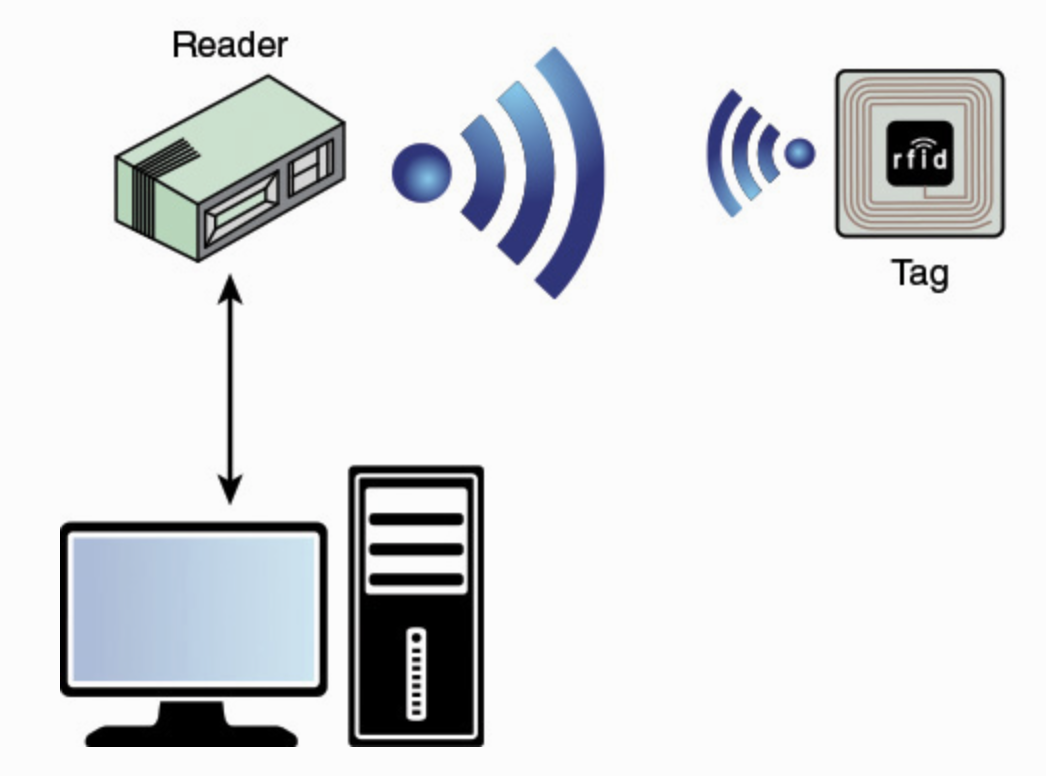
\includegraphics[width=0.80\textwidth,height=\textheight,keepaspectratio]{images/fig_5_10}
\caption{Elementi di un sistema RFID}
\label{fig:5_9}
\end{figure}

\chapter{The Internet of Things: Architecture and Implementation}\label{ch:chapter8}
\section{IoT Architecture}
Data la complessit� dell'IoT, � utile avere un'architettura che specifica gli elementi chiave e la loro interconnessione. Un'architettura IoT pu� avere i seguenti benefici:
\newline
- avere una lista con la quale essere in grado di valutare funzionalit� e completezza delle varie offerte proposte dai venditori.
\newline
- fornisce una guida agli sviluppatori su quali funzioni sono necessarie nell'IoT e come quest'ultime funzionano insieme.
\newline
- pu� servire come un framework per la standardizzazione, promuovere l'interoperabilit� e ridurre i costi. \cite{tutorial}, \cite{referenceArchitectures}

\subsection{ITU-T IoT Reference Model}
Il modello ITU-T si concentra in maggior dettaglio sui componenti fisici attuali dell'ecosistema IoT. Questa � un'analisi fondamentale poich� rende visibili gli elementi dell'IoT che devono essere interconnessi, integrati, gestiti e resi disponibili per le applicazioni.
\newline
\newline
\textbf{Devices}
\newline
L'unico aspetto dell'IoT, comparato con altri sistemi network, � la presenza di un numero di oggetti fisici e dispositivi diverso dai dispositivi informatici o di elaborazione dati. Il modello ITU-T vede l'IoT funzionante come una rete di dispositivi che sono strettamente collegati agli oggetti. Sensori ed attuatori interagiscono con gli oggetti fisici nell'ambiente. 
\newline
I dispositivi di acquisizione dati leggono / scrivono dati su oggetti fisici tramite l'interazione con un dispositivo di trasporto/supporto dati associato a un oggetto fisico.

\begin{figure}[htbp]
\centering
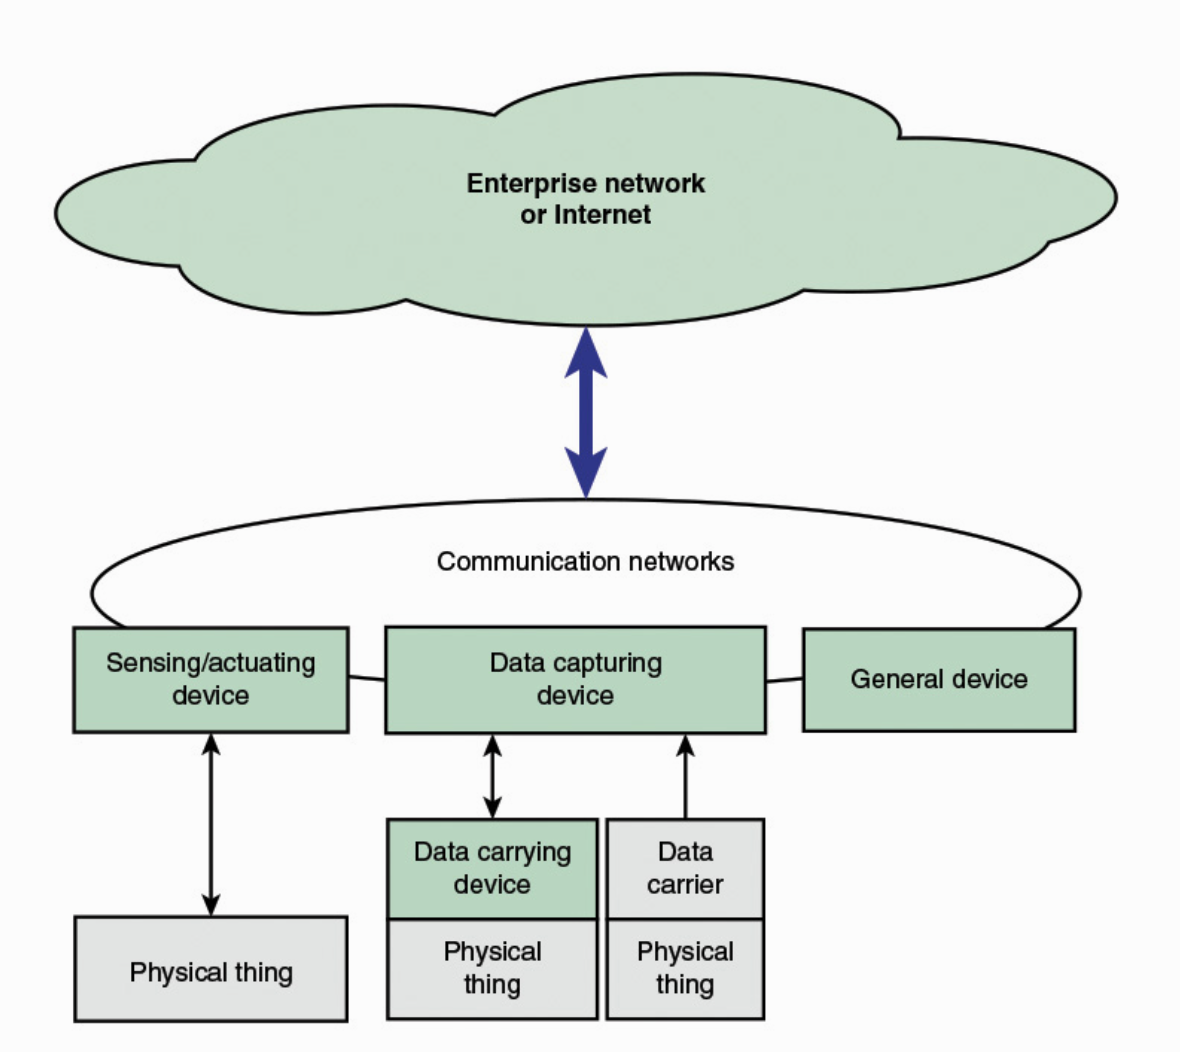
\includegraphics[width=0.80\textwidth,height=\textheight,keepaspectratio]{images/fig_6_1}
\caption{Tipi di dispositivi e la loro relazione con gli oggetti fisici}
\label{fig:6_1}
\end{figure}

\textbf{The Reference Model}
\newline
Il modello di riferimento del modello IOT ITU-T consiste in quattro strati con capacit� di gestione e di sicurezza che attraversano tutti gli strati.

\begin{figure}[htbp]
\centering
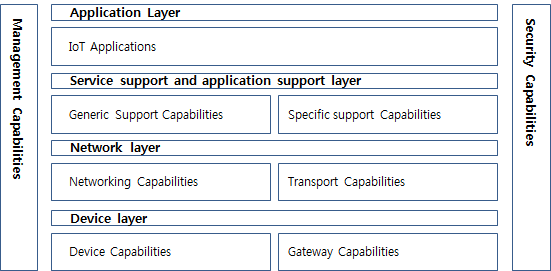
\includegraphics[width=0.80\textwidth,height=\textheight,keepaspectratio]{images/fig_6_2}
\caption{ITU-T Y.2060 IoT Reference Model}
\label{fig:6_2}
\end{figure}

Il \textbf{network layer} esegue due funzioni basiche. Le "networking capabilities" si riferiscono all'interconnessione fra i dispositivi e le porte. Le "transport capabilities" si riferiscono al trasporto dei vari servizi dell'IoT oltre alle informazioni collegate di controllo e gestione.
\newline
Il \textbf{service support and application support layer} fornisce delle funzionalit� che vengono usate dalle applicazioni. Un esempio comune riguarda l'elaborazione dei dati e la gestione del database.
\newline
L'\textbf{application layer} consiste di tutte le applicazioni che interagiscono con i dispositivi IoT.
\newline
Il \textbf{management capabilities layer} ricopre le tradizionali funzioni di rete come la gestione di guasti, configurazione e gestione delle prestazioni.
\newline
Il \textbf{security capabilities layer} include funzionalit� di sicurezza generiche indipendenti dalle applicazioni. 

\subsection{IoT World Forum Reference Model}
L'IoT World Forum � un evento annuale sponsorizzato dalle aziende che raggruppa insieme rappresentanti del business, governi ed accademie per promuovere lo sviluppo e l'adozione nel mercato dell'IoT. 
\newline
Il comitato per l'architettura nell'IoT World Forum, che include fra ke molte aziende colossi internazionali del calibro di IBM, Intel e Cisco i quali hanno rilasciato un modello di riferimento per l'IoT nel 2014. Questo modello � servito come framework di riferimento per aiutare l'industria ad accelerare lo sviluppo dell'IoT.
\newline
Questo modello di riferimento � un elemento complementare al modello di riferimento ITU-T, con la differenza che quest'ultimo si concentra maggiormente a livello di dispostivi e porte. Invece il modello IoT World Forum si concentra in maniera pi� ampia sullo sviluppo di applicazioni, middleware e funzioni di supporto per l'IoT aziendale.

\begin{figure}[htbp]
\centering
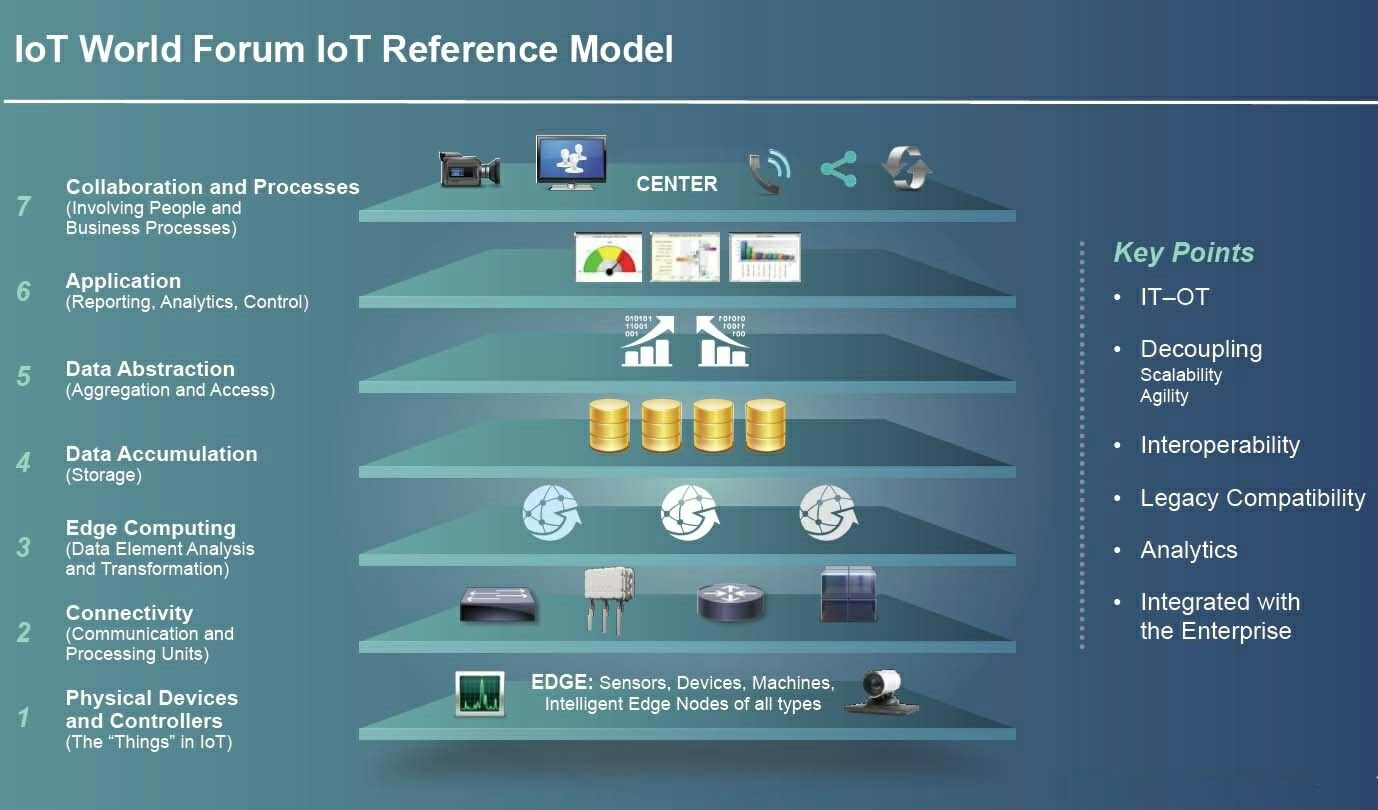
\includegraphics[width=0.80\textwidth,height=\textheight,keepaspectratio]{images/fig_6_3}
\caption{IoT World Forum Reference Model}
\label{fig:6_3}
\end{figure}

- \textbf{Semplifica}: aiuta ad abbattere un sistema complesso rendendolo pi� comprensibile.
\newline
- \textbf{Chiarifica}: fornisce informazioni aggiuntive per identificare precisamente i livelli dell'IoT e stabilisce una terminologia comune.
\newline
- \textbf{Identifica}: identifica dove specifici tipi di processi sono ottimizzati nelle diverse parti del sistema.
\newline
- \textbf{Standardizza}: fornisce un aiuto alle industrie per permetter loro di creare prodotti ioT che lavorino fra di loro.
\newline
- \textbf{Organizza}: rende reale ed accessibile l'IoT, invece che semplicemente concettuale.

\section{IoT Implementation}
Abbiamo visto due modelli di riferimento, i quali forniscono un'ottima panoramica delle funzionalit� ricercate durante la progettazione di un sistema IoT. Vediamo adesso un esempio della distribuzione di dispositivi e software IoT.  \cite{futureIoT}, \cite{roadmap}

\subsection{Cisco IoT System}
Nel 2015 Cisco ha introdotto una suite di prodotti integrati e coordinati, noti come \textit{Cisco IoT System}. La filosofia guida che ha guidato l'azienda era la previsione che entro la fine del 2020 ci fossero almeno 50 miliardi di dispositivi connessi ad Internet. Attualmente circa il 99\% degli oggetti nel mondo non � connesso ad internet, ma nel lungo processo di digitalizzazione che stanno seguendo le industrie e le citt� sono sempre pi� diffuse le soluzioni IoT.
\newline
Cisco IoT System affronta la complessit� della digitalizzazione offrendo una infrastruttura designata per gestire sistemi su larga scala di diverse piattaforme e il flusso di dati che queste creano. Il sistema consiste in una architettura basata su sei pilastri con l'obiettivo di ridurre la complessit� della digitalizzazione; inoltre Cisco ha proposto un buon numero di prodotti IoT ed il continuo rilascio e sviluppo di nuovi dispositivi. 

\begin{figure}[htbp]
\centering
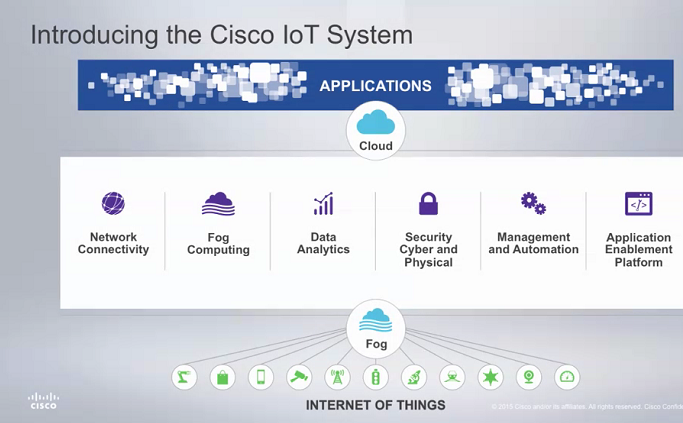
\includegraphics[width=0.80\textwidth,height=\textheight,keepaspectratio]{images/fig_6_4}
\caption{Cisco IoT System}
\label{fig:6_4}
\end{figure}

- \textbf{Networking connectivity}: include prodotti di routing, switching e wireless appositamente progettati.
\newline
- \textbf{Fog comoputing}: fornisco il fog computing di Cisco o la piattaforma di elaborazione dati IOx.
\newline
- \textbf{Data analytics}: un'infrastruttura ottimizzata per implementare l'analisi dei dati, sfruttando sia il \textit{Cisco Connected Analytics Portfolio} che software di terze parti.
\newline
- \textbf{Security}: unifica la cyber-security e la physical-security per fornire vantaggi operativi e incrementare la protezione sia per le risorse fisiche che digitali. Un esempio � il TrustSec di Cisco.
\newline
- \textbf{Management and automation}: strumenti per la gestione degli endpoints e delle applicazioni.
\newline
- \textbf{Application enabled platform}: un set di APIs per permettere di sviluppare e produrre applicazioni compatibili con le capacit� del sistema IoT.



\chapter{Architettura del sistema}\label{ch:chapter9}
L'idea alla base del sistema IoT � quella di progettare una catena di produzione tipica di un'industria 4.0 attraverso l'utilizzo di SDN-Wise. Per lo sviluppo del sistema sono state affiancate le tecnologie di SDN-Wise, approfondite nei capitoli precedenti, con metodologie per effettuare le lavorazioni e monitorare l'andamento della catena industriale con prevenzione per gusti e malfunzionamenti. 
\newline 
Il sistema progettato prevedeva gi� all'interno tutti i meccanismi previsti dal SDN-Wise e sono stati implementati i seguenti meccanismi per la realizzazione finale:
\newline
- \textbf{sondaggio}: per monitorare l'ambiente � stato implementato un sistema di consenso distribuito, nella quale ogni nodo che partecipa al sondaggio comunica con gli altri nodi partecipanti, invece di avere una comunicazione unicast con il Controller.
\newline
- \textbf{attuatori e meccanismo di prevenzione guasti}: per la prevenzione guasti o errore di lavorazione durante la catena industriale sono stati implementati dei meccanismi di allarme e dei nuovi mote che compiessero delle azioni per salvaguardarlo.

\section{Attori partecipanti}
Nel sistema progettato gli attori principali sono tre e partecipano tutti attivamente per la realizzazione della catena industriale con lavorazione e risposta ai guasti e agli errori di lavorazione. In particolare questi tre elementi sono \textbf{Controller}, \textbf{Sink} e  \textbf{Mote}. Di seguito verranno analizzati singolarmente in maniera pi� approfondita. 
\subsection{Controller}
Il Controller � un entit� logica centralizzata, che ha la visione completa e aggiornata della topologia della rete e delle relazioni tra i nodi. Per interfacciarsi con la rete, esso apre una comunicazione TCP con il Sink, attraverso la quale il Controller pu� inviare pacchetti per la modifica della topologia della rete o per riceve pacchetti sullo stato dei nodi o delle richieste da parte di essi. 
\newline 
\begin{figure}[htbp]
\centering
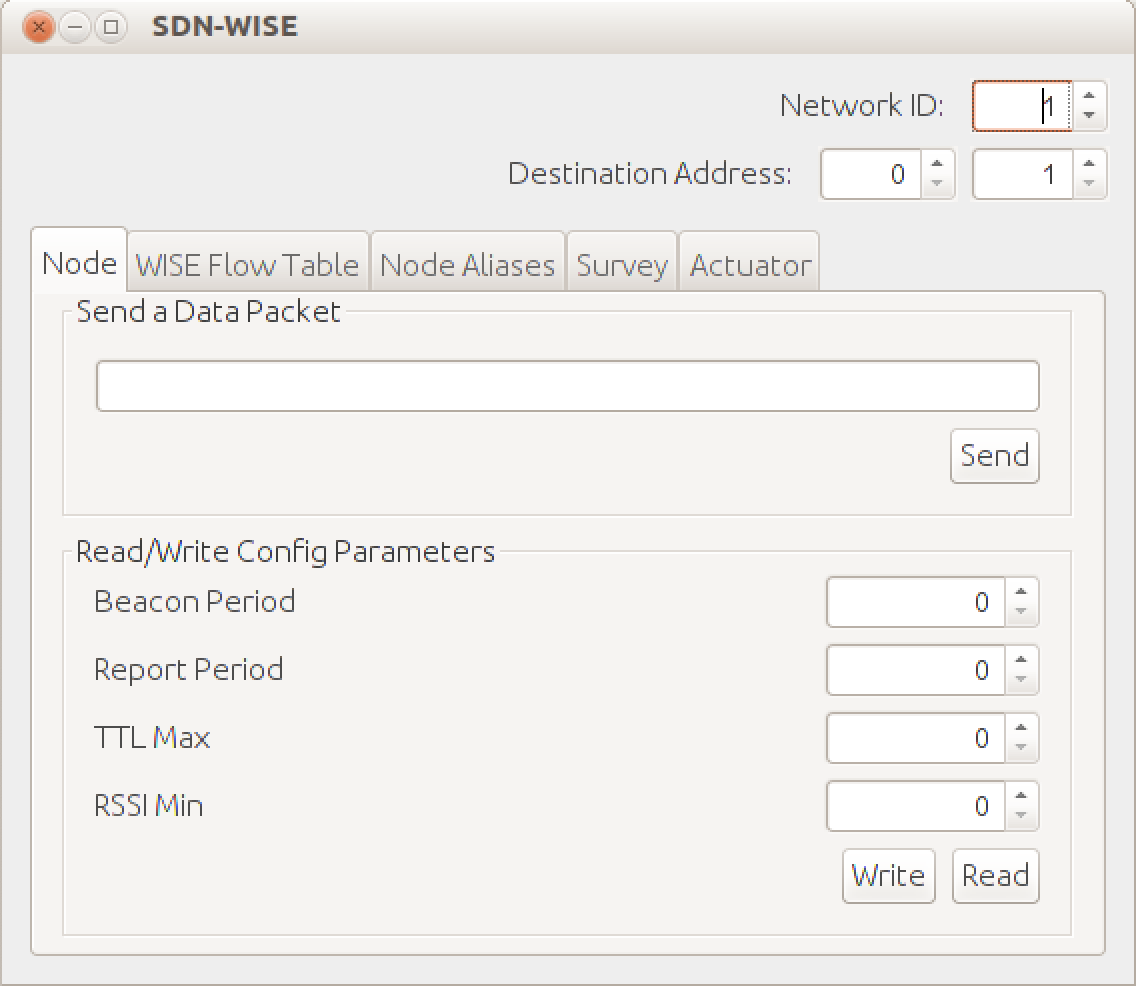
\includegraphics[width=0.60\textwidth,height=\textheight,keepaspectratio]{images/fig_9_1}
\caption{Pannello del Controller}
\label{fig:6_4}
\end{figure}
\newline
Nel sistema progettato il Controller si presenta come nella figura soprastante. Questo pannello da la possibilit� all'Operatore, che ha il compito di monitorare la catena industriale e di avviare le lavorazioni, di inviare pacchetti di vario genere per monitorare il funzionamento dell'intero sistema o per modificare la struttura topologica.
\newline
Per il monitoraggio della rete, nel sistema � previsto un pannello che riproduce la topologia della rete basandosi sui pacchetti dei report, pacchetti nel quale ogni nodo specifica i suoi vicini. Un esempio � mostrato in figura:
\newline
\begin{figure}[htbp]
\centering
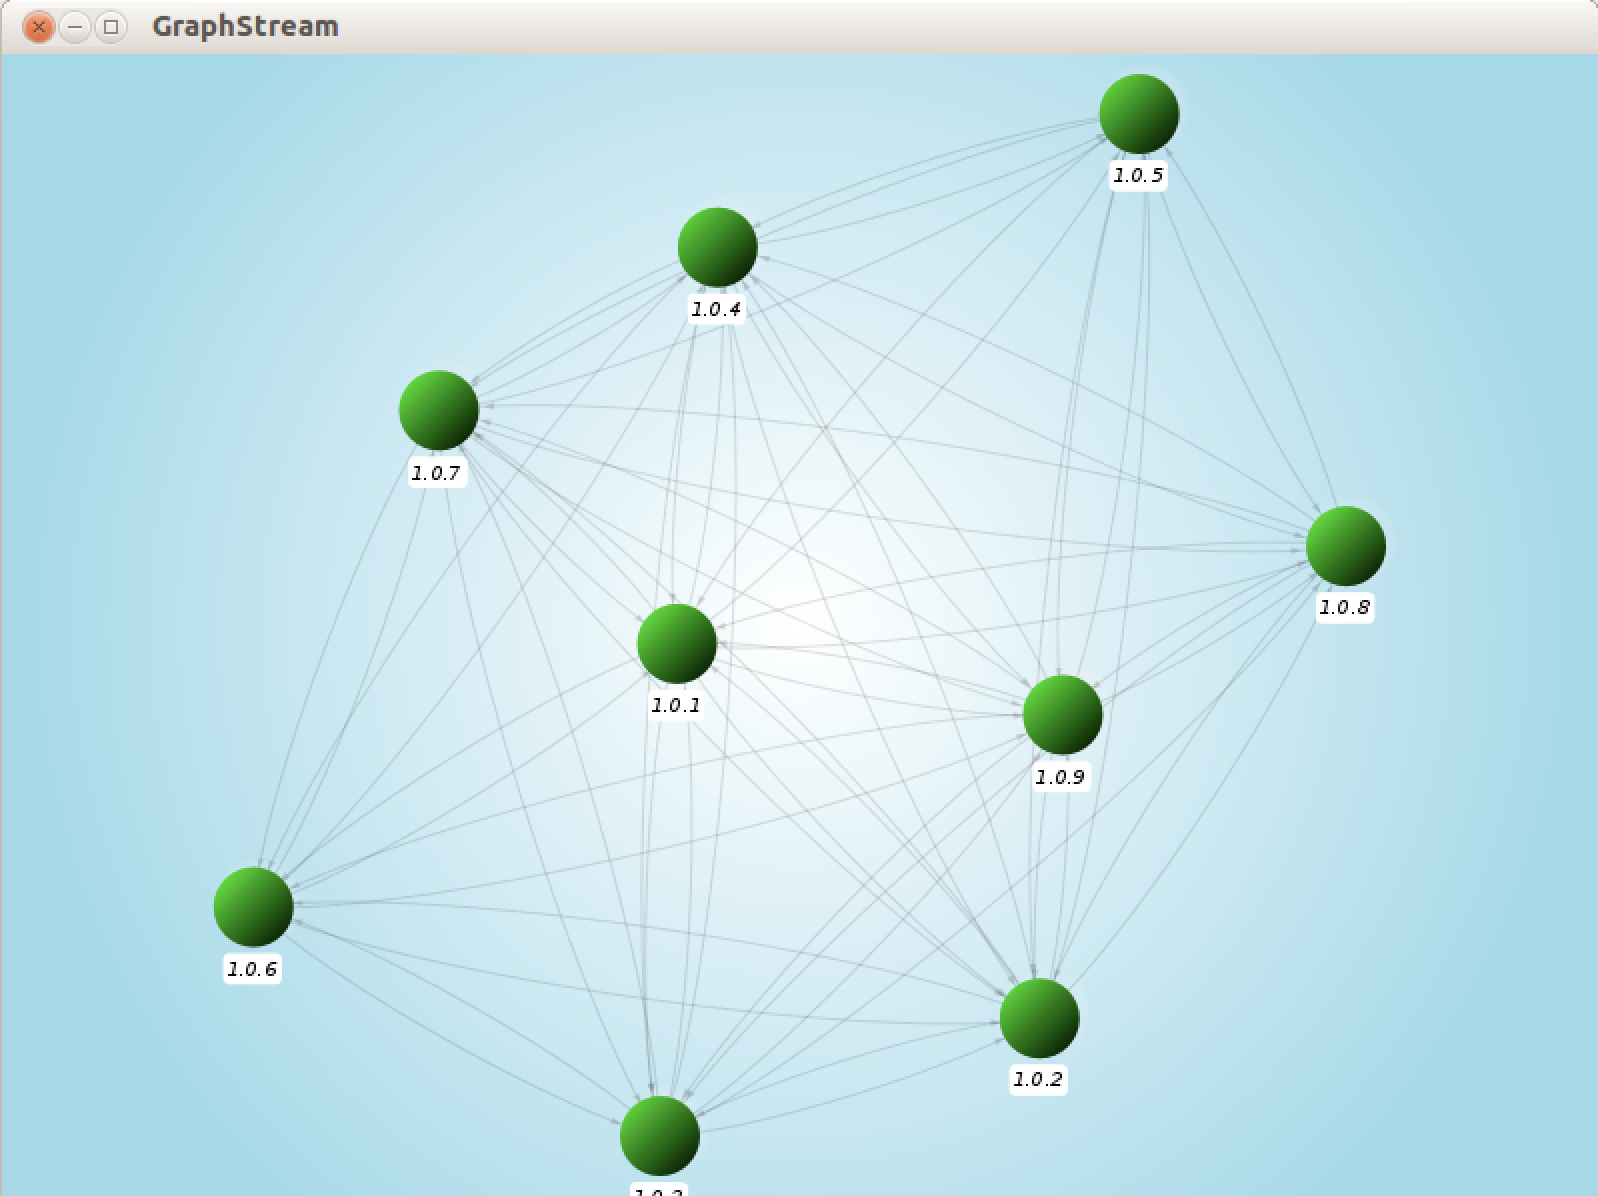
\includegraphics[width=0.70\textwidth,height=\textheight,keepaspectratio]{images/fig_9_2}
\caption{Topologia Rete}
\label{fig:6_4}
\end{figure}
\newline
\subsubsection{Survey e Actuator}
All'interno del pannello del controller sono presenti due campi, Survey e Actuator. 
\newline
\begin{figure}[htbp]
\centering
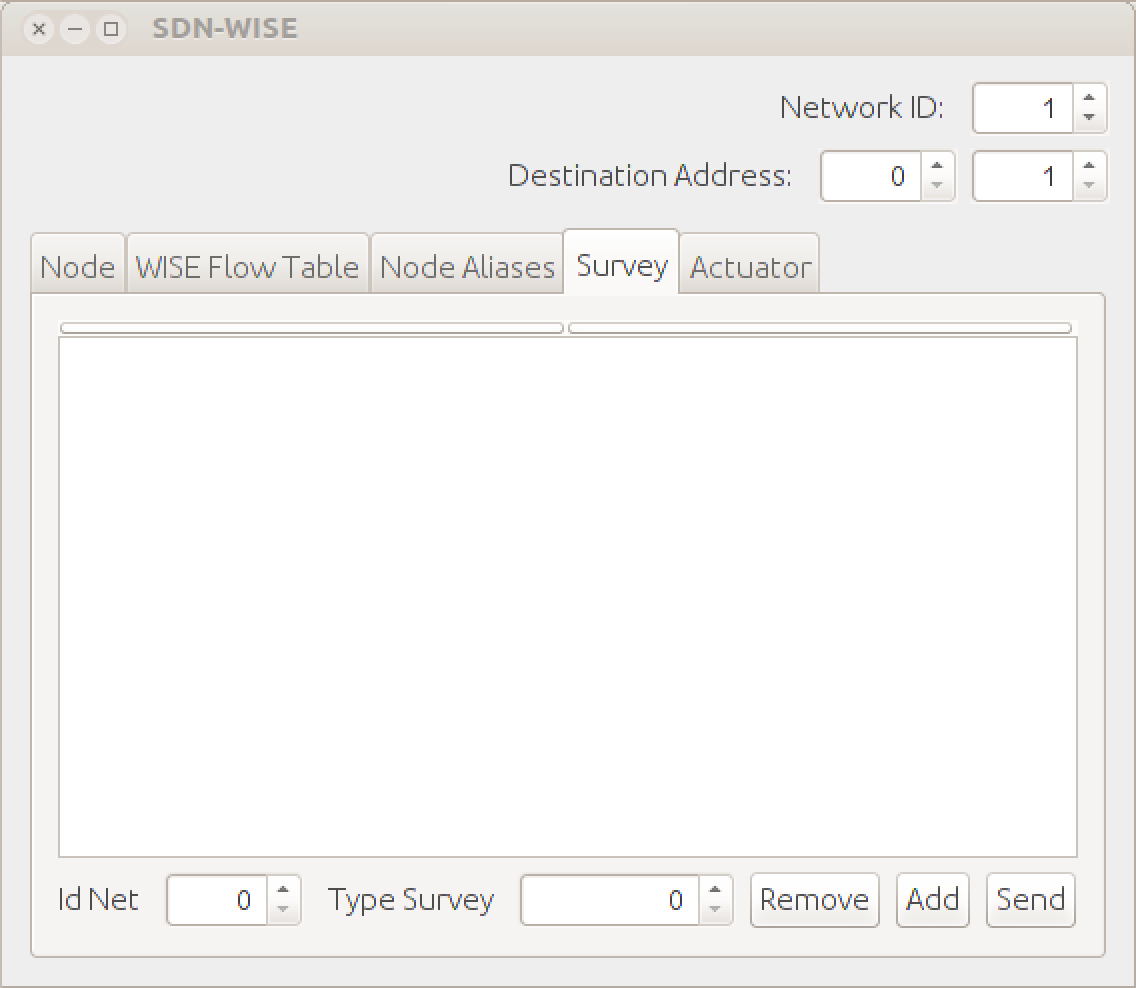
\includegraphics[width=0.70\textwidth,height=\textheight,keepaspectratio]{images/fig_9_1_1}
\caption{Pannello Survey}
\label{fig:6_4}
\end{figure}
\newline
Quest'ultimi presentano una tabella a due colonne che rappresentano rispettivamente l'High Adress e Low Adress degli indirizzi dei nodi che partecipano. I due Spinner in basso al pannello rappresentano ID della rete, che andr� a inserirsi nel primo byte dell'Header, e il TYP(azione o sondaggio), che sar� il primo byte del payload. 
\newline
\newline
Di fianco ai due Spinner, sono presenti tre bottoni, remove, Send e Add; questi tre attivano tre metodi differenti:
\newline
- \textbf{Remove}: rimuove un nodo dalla tabella.
\newline
- \textbf{Add}: inserisce un nuovo nodo nella tabella; per inserirlo, una volta cliccato il pulsante add apparir� il seguente pannello aggiuntivo:
\newline
\newline
\begin{figure}[htbp]
\centering
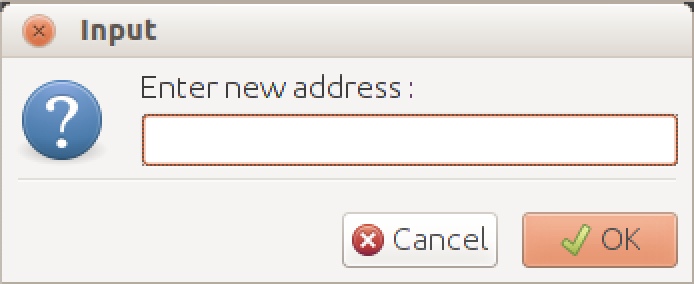
\includegraphics[width=0.60\textwidth,height=\textheight,keepaspectratio]{images/fig_9_1_2}
\caption{Pannello newAddress}
\label{fig:6_4}
\end{figure}
\newline
\newline
- \textbf{Send}: invia il pacchetto al Sink.
\newline
I nodi della tabella, ogni volta che viene compiuto l'evento add, vengono aggiunti a una lista di NodeAdress; premuto il tasto send, invece, viene creata la lista di valori, inizialmente inizializzata a zero, e viene creato il pacchetto per inviarlo al Sink.
\subsection{Sink}
Il Sink � un nodo della rete ed � l'unico nodo che pu� dialogare con il Controller; questo fa si che gli altri nodi della rete conoscano il suo indirizzo in modo tale che tutti possano inviare richieste o report al Controller. Dal Sink passano tutti i pacchetti , questo lo rende il perno fondamentale della rete ed � grazie a lui che il Controller pu� conoscere ogni dettaglio della rete. All'interno del framework \textit{Cooja} il Sink � raffigurato con il colore verde.
\newline
\begin{figure}[htbp]
\centering
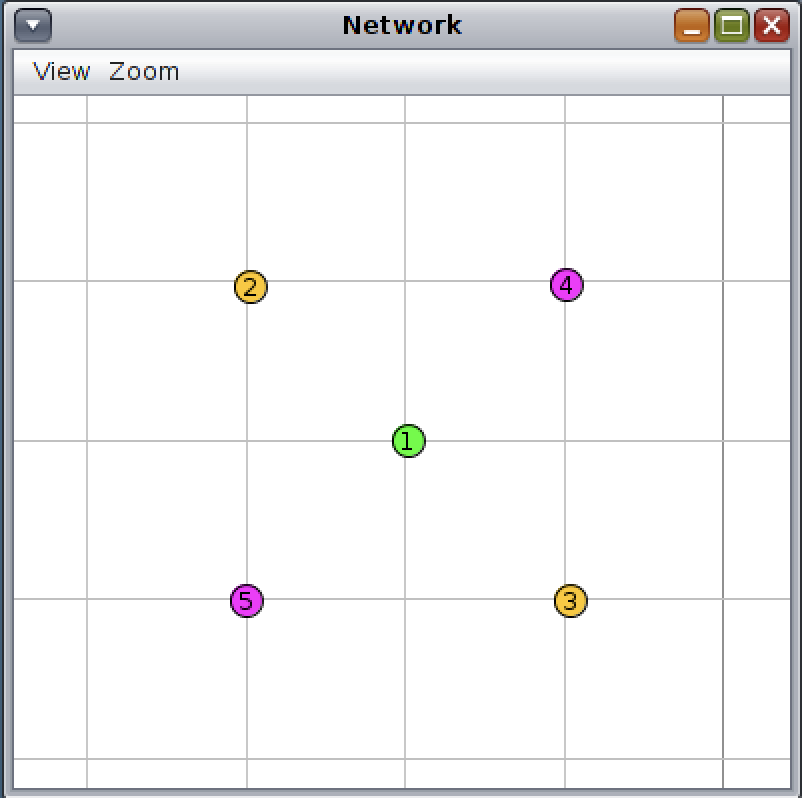
\includegraphics[width=0.60\textwidth,height=\textheight,keepaspectratio]{images/fig_9_3}
\caption{Sink, Mote e Actuator Mote}
\label{fig:6_4}
\end{figure}
\newline
\subsection{Mote}
I mote sono i restanti nodi della rete, i compiti principali sono di dialogare tra loro e con il Sink attraverso l'invio di pacchetti \textit{beacon,report,request}. 
\newline
Nel sistema progettato i mote si dividono in due categorie:
\newline
- \textbf{Mote}: hanno il compito di monitorare l'ambiente, monitorando i dati richiesti dal sondaggio.
\newline
- \textbf{Actuator Mote}: gli Actuator Mote hanno il compito di attuare un'azione specifica per prevenire un danno ambientale.
\newline
All'interno del framework \textit{Cooja} il Mote � raffigurato con il colore giallo, mentre l'Actuator Mote con il colore viola.

\chapter{Framework utilizzati}\label{ch:chapter10}
La maggior parte delle sfide legate alle WSN non sono ancora state gestite adeguatamente. Anche se il paradigma SDN promette un enorme riduzione del consumo di energia da parte dei nodi, le entit� di queste affermazioni devono essere valutate e quantificate.
A tal proposito SDN-WISE offre un simulatore di rete, chiamato Cooja, che gira sul sistema operativo Contiki e consente di semplifcare la produzione di applicazioni per le WSN, nonch� la simulazione per testing e debugging. Inoltre pu� essere utilizzato a scopo didattico per gli studenti.
Le simulazioni vengono svolte con topologie di rete differenti, cos� come il numero di messaggi circolanti in rete verr� variato. \cite{github}

\section{Contiki}
Contiki � il sistema operativo open source per creare reti IoT wireless a bassa potenza. � stato sviluppato presso lo Swedish Institute of Computer Sciences da Adam Dunkels e il suo team. � scritto nel linguaggio di programmazione C, cos� come ogni sua estensione. Contiki � un sistema operativo altamente portatile ed � gi� stato distribuito su diverse piattaforme utilizzanti diversi tipi di processori. La maggior parte di esse spesso usano Texas Instruments MSP-430 o Atmel ATmega come microcontrollori.
Contiki utilizza un modello di programmazione basato su eventi per gestire la programmazione concorrente. Il suo principale vantaggio � che tutti i processi condividono uno stack consentendo un oneroso risparmio di memoria. Questo modello viene realizzato mediante dei Protothread, i quali forniscono blocking wait, condizionato o meno, per salvare lo stato in modo continuativo. Quando il Protothread viene riattivato, riparte dall'istruzione successiva. Contiki usa anche il cosiddetto Rime stack, una pila di comunicazione per reti di sensori molto leggera, in quanto gli strati sono semplici e hanno piccole intestazioni di pochi byte. Rime supporta anche il riutilizzo del codice col principale scopo di semplificare l'implementazione delle WSN.
Contiki supporta sia IPv6 che IPv4, nonch� i pi� recenti standard per le reti wireless a bassa potenza, come 6lowpan, RPL e CoAP. La sua popolarit� lo ha portato in numerosi sistemi, quali contatori di energia elettrica, moni- toraggio industriale, sistemi di allarme, monitoraggio remoto della casa, del suono nella citt�, delle radiazioni e via dicendo.
L'ultima versione Contiki 3.0 � stata rilasciata il 26 agosto 2015


\section{Cooja}
Cooja � il simulatore di rete per Contiki. � un'applicazione Java-based con interfaccia grafica basata sullo standard Java Swing toolkit. Cooja supporta la simulazione per mezzo di onde radio e l'integrazione con tool esterni per fornire funzionalit� aggiuntive. L'emulazione pu� avvenire sia a un livello meno dettagliato, in modo che sia pi� veloce e consenta la simulazione di reti pi� grandi, sia a livello hardware, pi� lento ma che consente un'ispezione precisa del comportamento del sistema.
\newline
Questo strumento ha due pacchetti software per la simulazione: Avrora e MSPSim. Il primo � usato da Cooja per l'emulazione di dispositivi basati su Atmel AVR, mentre il secondo per quelli basati su TI MSP430. La mag- gior parte delle piattaforme usano Microcontrollori di questo tipo, pertanto MSPSim � il pacchetto software pi� utilizzato.
Cooja pu� simulare pi� piattaforme, come TelosB, SkyMote, Zolertia Z1 mo- te, Wismote, ESB, MicaZ mote, ed � molto utile per lo sviluppo e il debugging di applicazioni per Contiki in quanto permette agli sviluppatori di:
\newline
- testare il loro codice e i sistemi prima di eseguirlo sull'hardware reale.
\newline
- stimare i consumi energetici dei nodi
\newline
- mostrare trasmissioni e ricezioni radio.
\newline
Per avviare Cooja � necessario disporsi nella cartella che lo contiene (nello specifico \textit{sdn-wise-contiki z1/contiki/tools/cooja} ) e invocare il comando \textit{ant run} dal terminale. Cooja partir� con una finestra blu vuota non appena la compilazione sar� conclusa.
\newline
\begin{figure}[htbp]
\centering
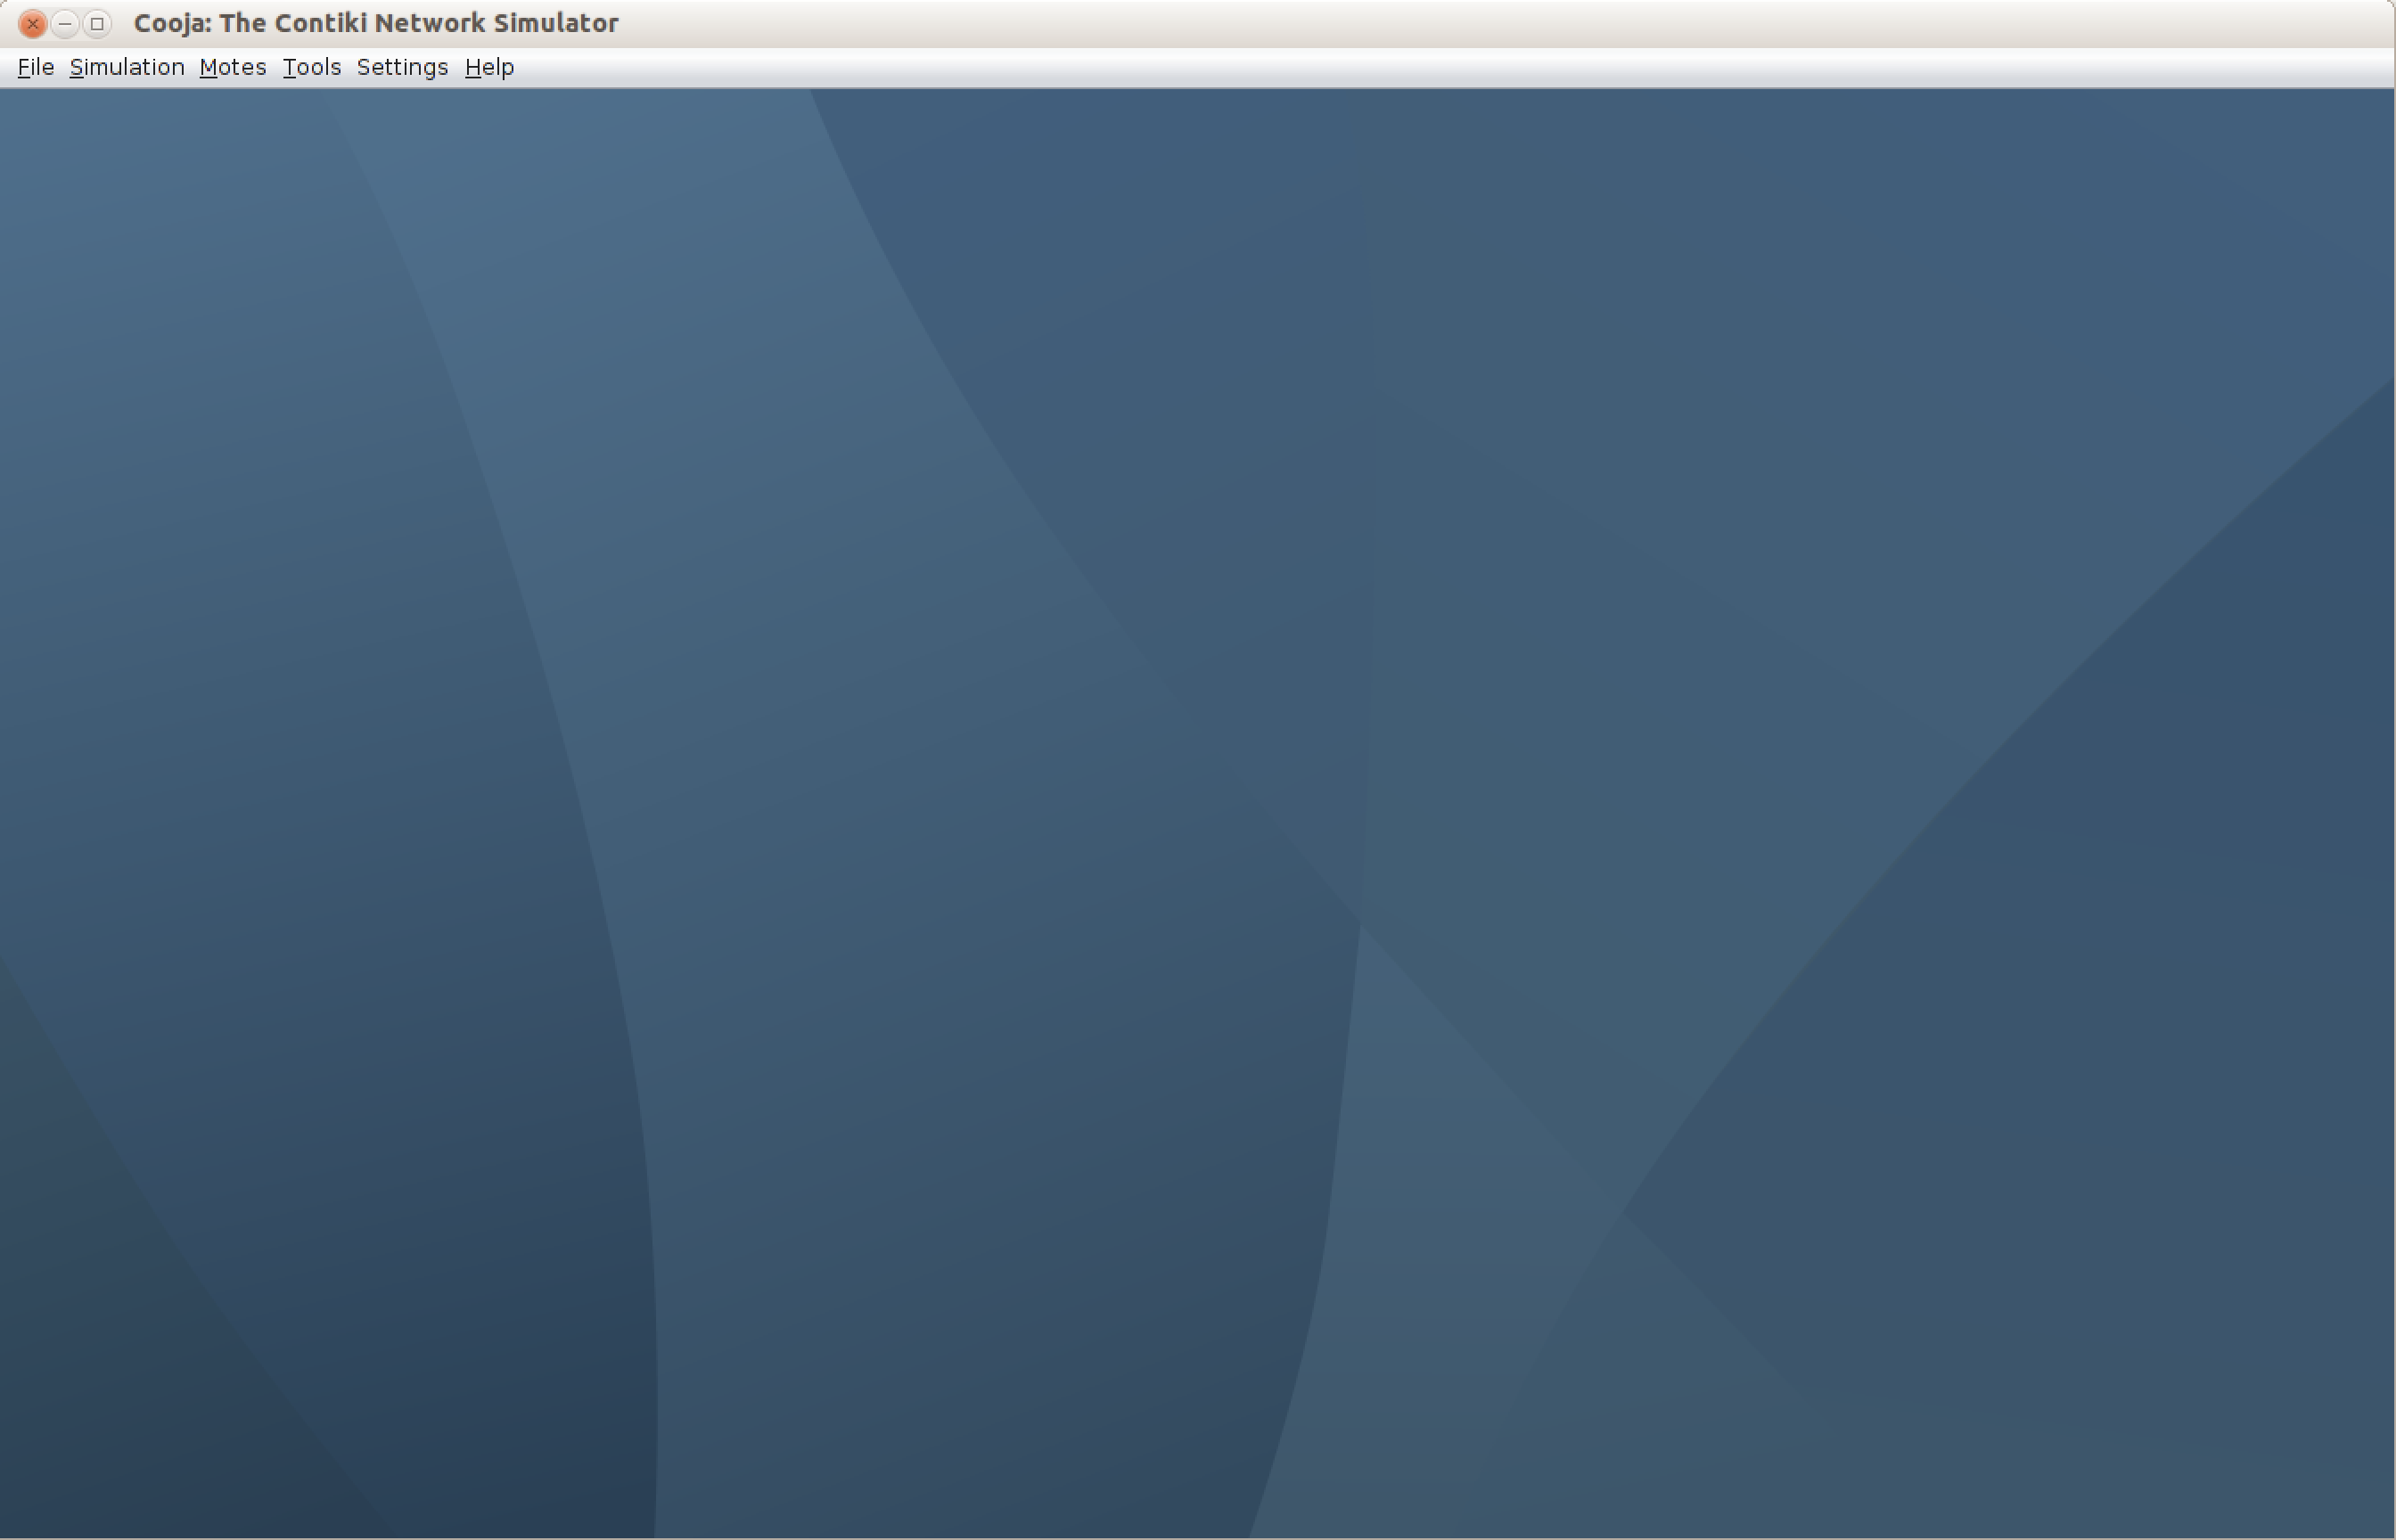
\includegraphics[width=0.60\textwidth,height=\textheight,keepaspectratio]{images/fig_10_1}
\caption{Finestra iniziale simulatore Cooja}
\label{fig:6_4}
\end{figure}
\newline
La prima cosa da eseguire � aggiungere una estensione che mi permette di aggiungere i mote e i sink che ho modificato nel programma sdn-wise-java. Per aggiungere questa estensione occorre cliccare su \textit{Settings --> Cooja Extension}.
\newline
\begin{figure}[htbp]
\centering
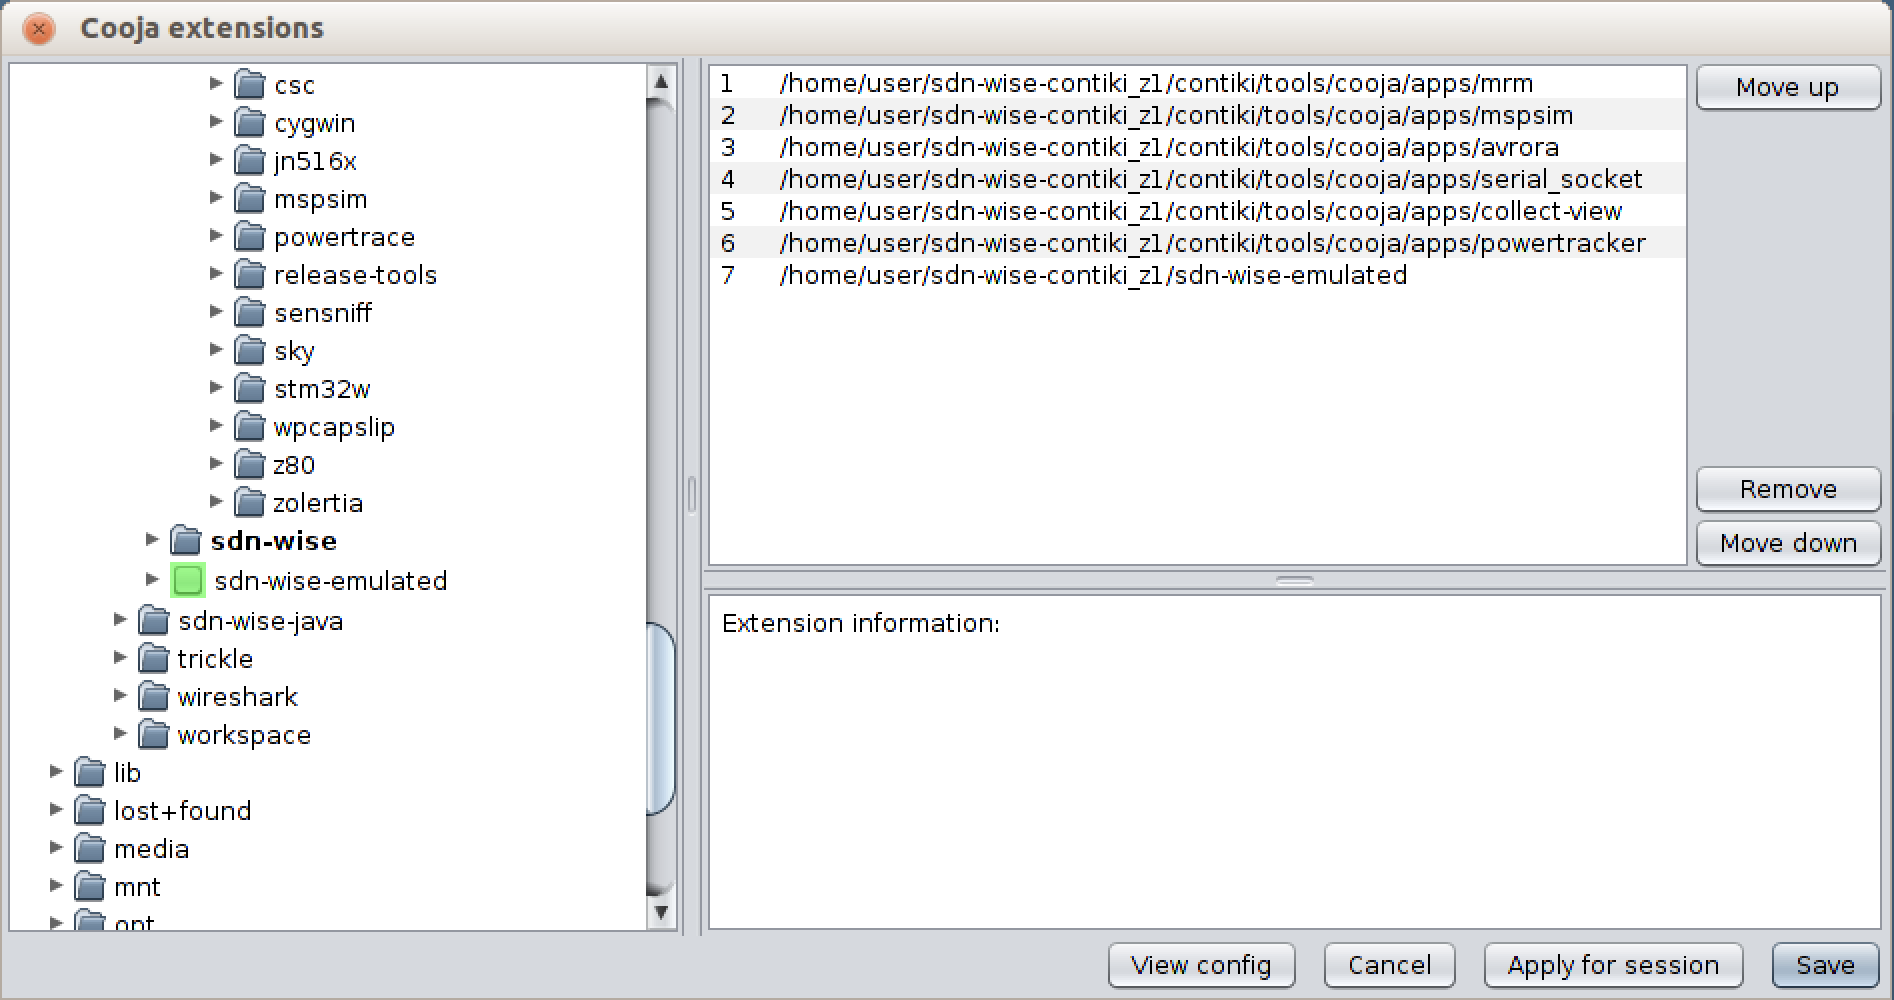
\includegraphics[width=0.60\textwidth,height=\textheight,keepaspectratio]{images/fig_10_2}
\caption{Aggiungere estensione per Cooja}
\label{fig:6_4}
\end{figure}
\newline
Una volta aggiunta questa estensione possiamo creare una nuova simulazione (\textit{File --> New Simulation}). Viene richiesto ora di inserire un nome per la simulazione, dopodich� ci troveremo di fronte al seguente pannello di Cooja:  
\newline
\begin{figure}[htbp]
\centering
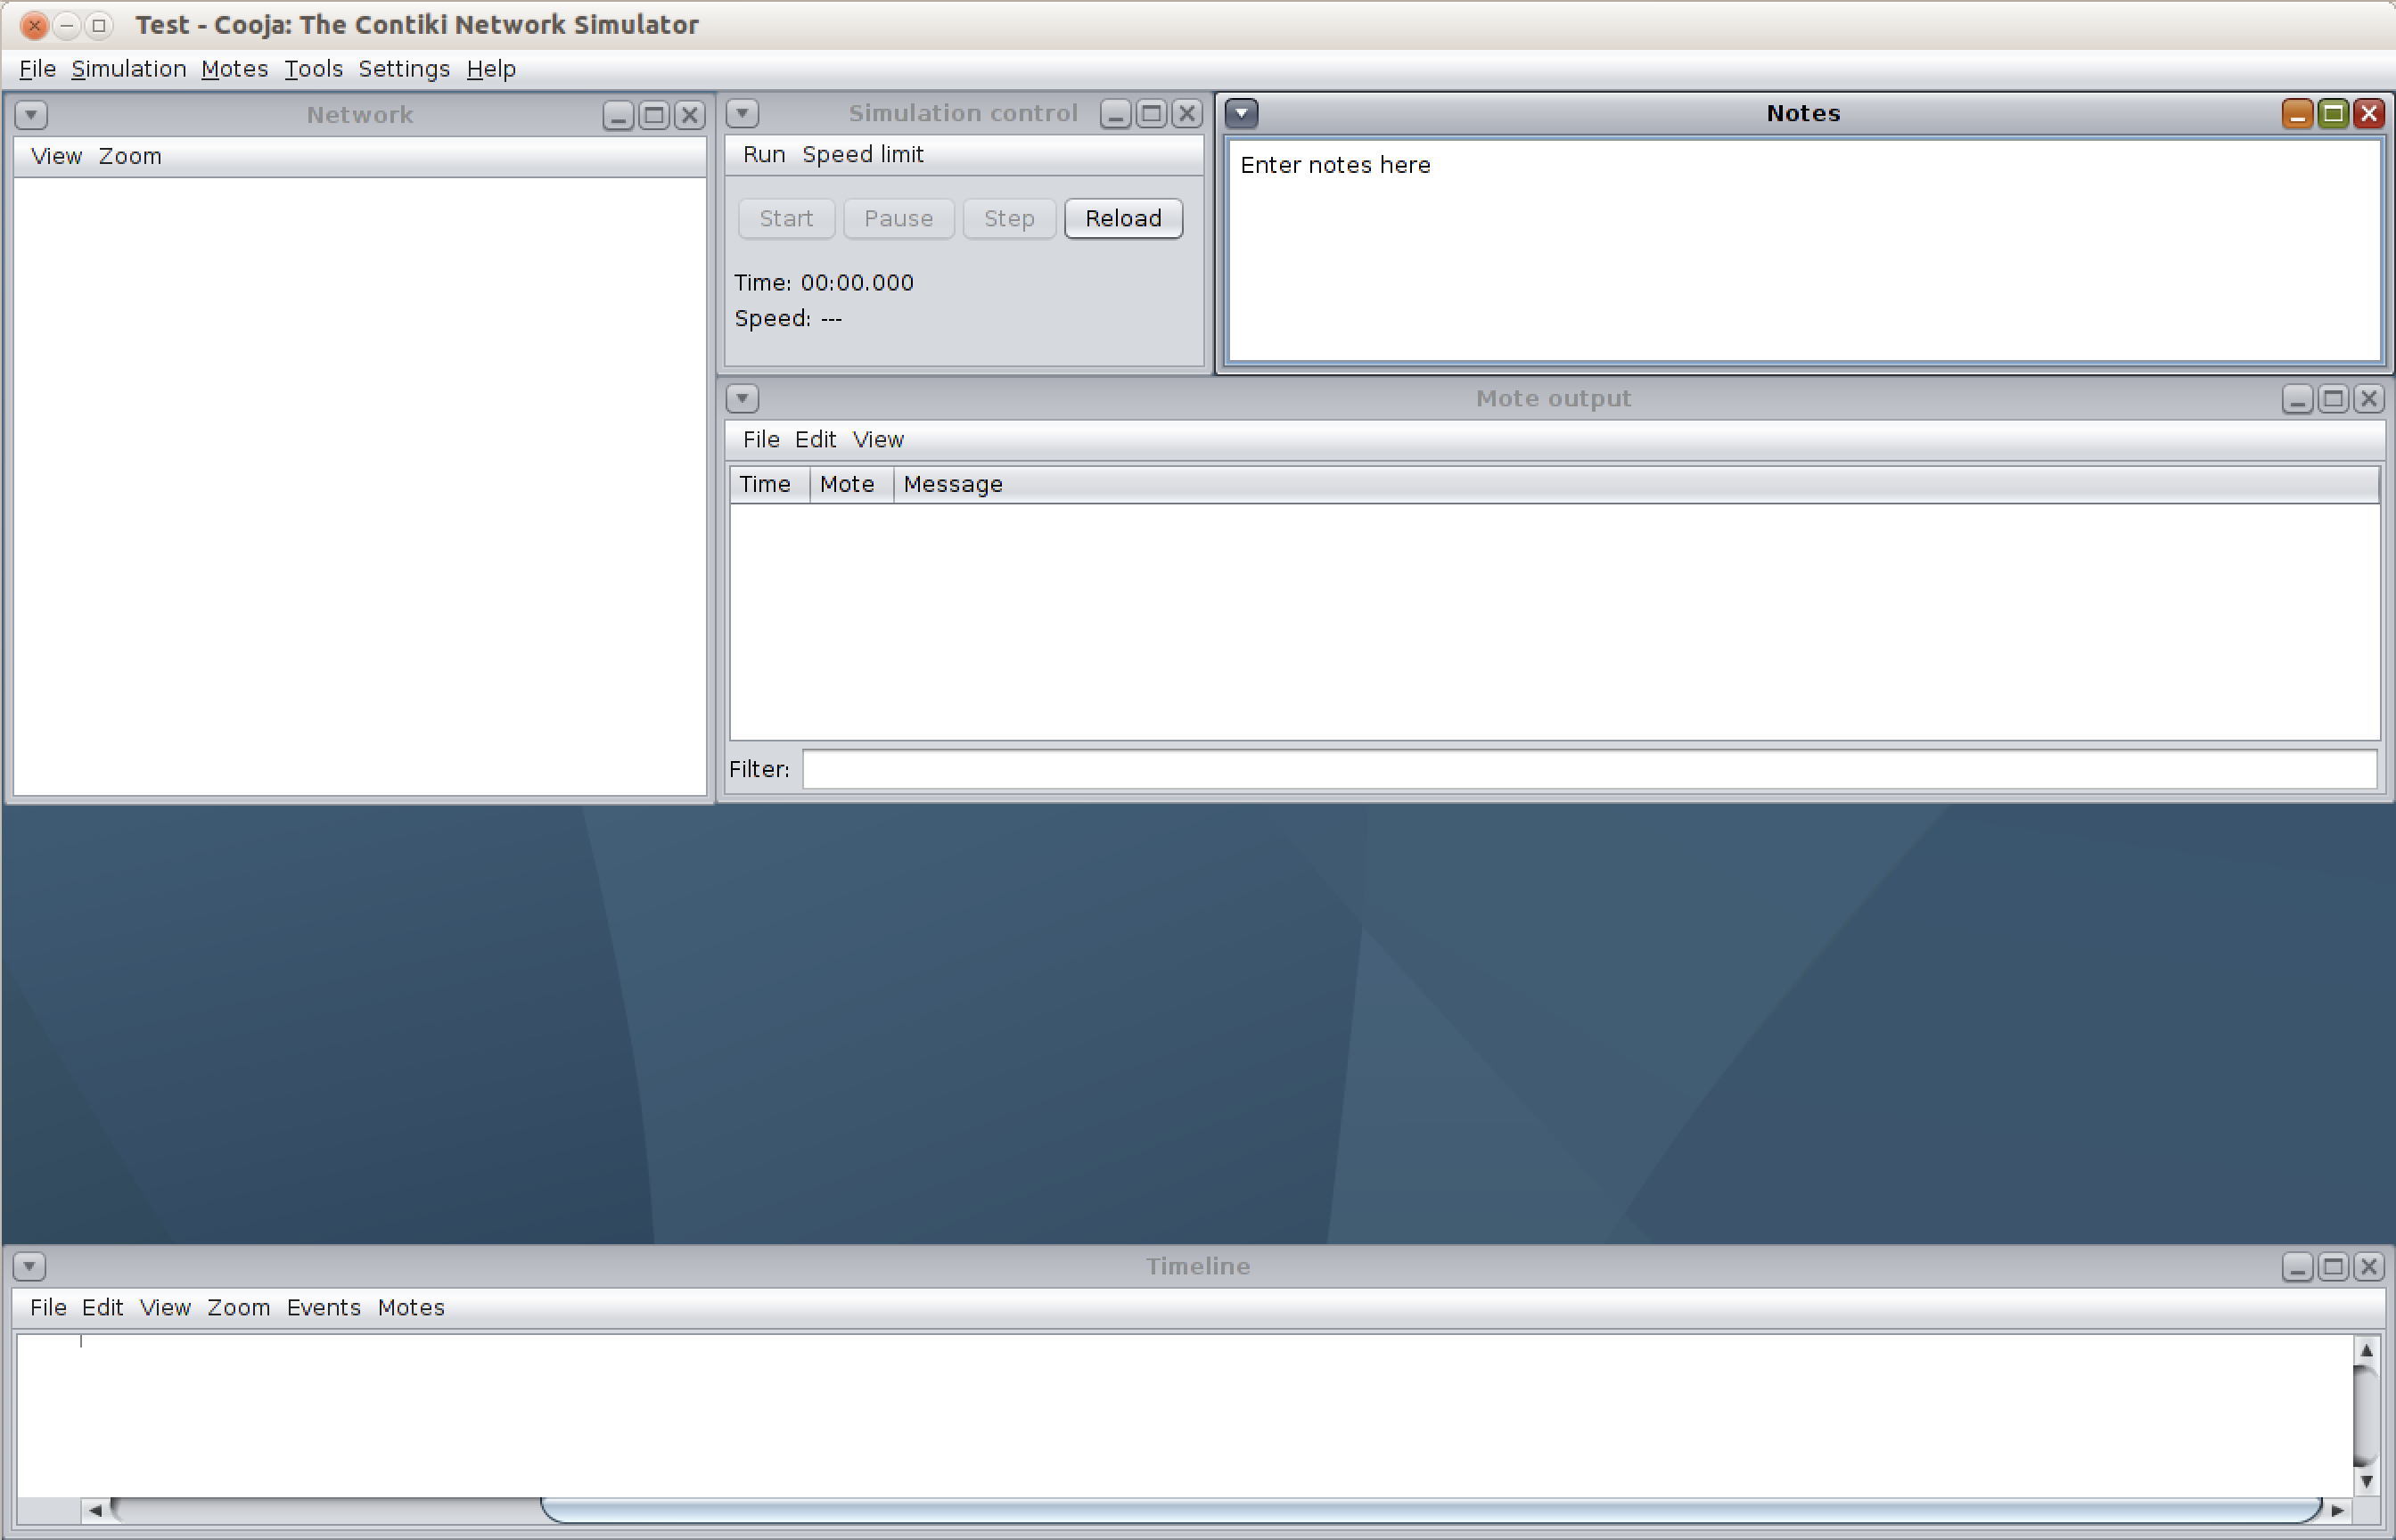
\includegraphics[width=0.60\textwidth,height=\textheight,keepaspectratio]{images/fig_10_3}
\caption{Pannello simulazione Cooja}
\label{fig:6_4}
\end{figure}
\newline
Cliccando su \textit{Mote --> Add motes --> Create new mote type} e scegliere tra i vari \textit{SDN-WISE Emulated Mote/Sink/Actuator Mote/Actuator Sink} in base alla simulazione che si vuole realizzare. 
\newline
\begin{figure}[htbp]
\centering
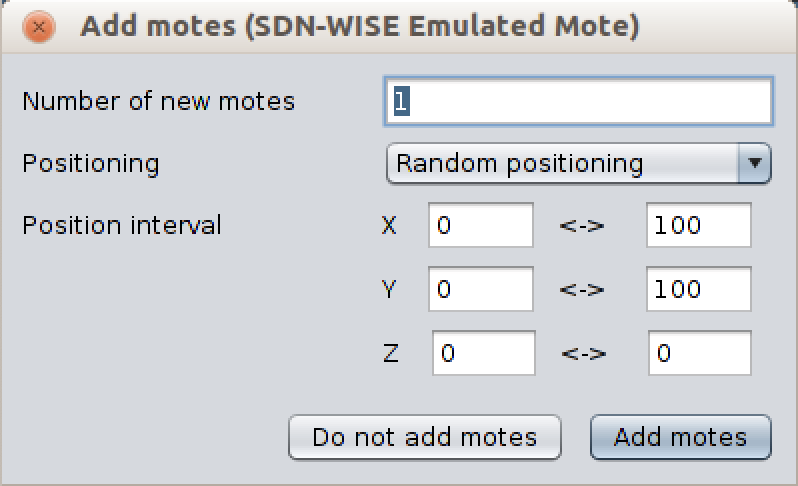
\includegraphics[width=0.60\textwidth,height=\textheight,keepaspectratio]{images/fig_10_4}
\caption{Aggiunta Mote}
\label{fig:6_4}
\end{figure}
\newline
Il simulatore chieder� quanti mote aggiungere e in quale posizione e li inserir� come richiesto. 
\newline
\newline
Nella figura 10.3 sono presenti dei tools di Cooja che verranno descritti brevemente:
\newline
- \textbf{Network}:  mostra la disposizione dei nodi della rete.Si pu� visualizzare anche la loro posizione il loro Id, il loro tipo, e la copertura radio.
\newline
- \textbf{Simulation Control}: viene usato per far partire, stoppare, ricaricare la simulazione e indica anche il tempo trascorso.
\newline
- \textbf{Mote Output}: Mostra tutti gli output dei vari nodi della rete.
\newline
- \textbf{Notes}: un semplice Notepad per prendere appunti sulla simulazione in corso.
\newline
- \textbf{Timeline}: mostra la timeline degli eventi come log output, cambio di canale, etc.

\section{IntelliJ IDEA e Linux Ubuntu 14.04}
Tra gli strumenti utilizzati vi sono anche l'ambiente di sviluppo \textit{IntelliJ IDEA} sviluppato da \textit{JetBrains}, e il sistema operativo \textit{Linux Ubuntu 14.04} alla base della macchina virtuale ospitante il framework.
\newline
Una volta lanciata la macchina virtuale � necessario eseguire queste semplici operazioni per eseguire il programma \textit{IntelliJ Idea}:
\newline
1 - aprire il terminale sulla macchina virtuale
\newline
2 - digitare \textit{cd /opt/idea/bin} e premere invio
\newline
3 - digitare \textit{./idea.sh} e premere invio
\newline
\newline
A questo punto si aprir� il programma \textit{IntelliJ Idea} e qualora non fosse stato ancora fatto � necessario caricare la cartella \textit{snd-wise-java} e tutti i suoi files. 
\newline
Nello specifico la cartella \textit{snd-wise-java} contiene tre macro package:
 \newline
- \textbf{core}: contiene tutte le informazioni riguardante i pacchetti scambiati dai nodi SDN-WISE e le informazioni che riguardano le Flow Tables.
\newline
- \textbf{control}:  contiene tutte le informazioni riguardante il Controller, dalla sua creazione alle se funzionalit�; contiene il package network graph, dove al suo interno viene creato il visual network graph. Inoltre � presente anche il package loader dove � presente il file che carica il progetto SDN-WISE.
\newline
- \textbf{data}: contiene tutte le informazione riguardante i nodi della rete, dalla creazione alle loro funzionalit� e tutte le informazioni sulla batteria.
\newline
\newline
Una volta effettuati i cambiamenti al codice ed ai vari file, sempre all'interno di \textit{IntelliJ Idea} � necessario eseguire in sequenza queste operazioni:
\newline
- cliccare su \textit{View -> Tool Window -> maven} 
\newline
Una volta che si sar� aperto il pannello eseguire in successione i seguenti comandi:
\newline
- \textit{clean}
\newline
- \textit{install}.
\newline
Infine sempre da terminale eseguire:
\textit{sudo cp -avr /home/user/sdn-wise-java/data/target/sdn-wise-data-4.0.1-SNAPSHOT-jar-with-dependencies.jar} 
\newline
\textit{/home/user/sdn-wise-contiki z1/sdn-wise-emulated/lib/sdn-wise-data.jar}
\newline
\newline
A questo punto � possibile lanciare la simulazione come abbiamo visto in precedenza. Per semplificare tutte queste operazioni ripetitive e meccaniche, � stato creato uno script. Il file in questione � stato chiamato \textit{compile.sh} ed una volta eseguite le varie modifiche � sufficiente scrivere direttamente nel terminale di \textit{IntelliJ Idea}:
\newline
- \textit{bash compile.sh}
\newline
\newline
A questo punto, mentre contestualmente viene lanciata la simulazione, baster� cliccare il pulsante \textit{run} su \textit{IntelliJ Idea} ed appariranno a schermo il controller SDN-WISE ed il GraphStream.

















\chapter{Simulazioni}\label{ch:chapter11}
\section{Scenari Analizzati}
In questo capitolo verranno discussi quattro tipi di simulazioni effettuate sul sistema per simulare vari scenari reali che si potrebbero presentare in una catena industriale. Per spiegare al meglio la simulazione e come i vari componenti del sistema interagiscono fra di essi, sono presenti un flow chart ed un sequence diagram per ogni tipo di scenario possibile.
\newline
Per effettuare le simulazioni sono state implementate quattro possibili combinazioni mediante l'utilizzo della probabilit�. In particolare:
\newline
- \textbf{Caso Ottimo}: fascia di probabilit� compresa fra 0.8 ed 1.0.
\newline
- \textbf{Caso Pessimo}: fascia di probabilit� compresa fra 0.0 e 0.2.
\newline
- \textbf{Caso Intermedio - RESTART}: fascia di probabilit� compresa fra 0.3 e 0.5.
\newline
- \textbf{Caso Intermedio - RELOAD}: fascia di probabilit� compresa fra 0.6 e 0.7.
\newline
L'obiettivo primario di questo progetto � stato quello di creare una riproduzione di una catena industriale IIoT 4.0 che fosse \textit{loop-less} ed altamente affidabile. Di seguito verr� descritto ogni possibile caso in maniera pi� approfondita.
\newline
Nella seconda parte del capitolo invece ci concentreremo sui risultati delle simulazioni, andando a misurare i ritardi all'interno dei vari casi e facendo una stima su come questo possa influenzare le quantit� prodotte in una catena industriale.  

\subsection{Scenario Caso Ottimo}
Il primo caso che andremo ad analizzare � il caso ottimo, ovvero quando la catena industriale IoT riesce ad eseguire tutte le lavorazioni senza rilevare anomalie o guasti. 
\newline
Il verificarsi del caso ottimo avviene con una probabilit� che oscilla fra il 70\% ed il 100\%, a seconda del caso che si vuole studiare ed analizzare; la probabilit� � piuttosto bassa, ma l'obiettivo � stato quello di analizzare in maniera critica la catena di montaggio, per permettere cos� di creare una catena \textit{high-quality} e con bassa tolleranza di errori o anomalie; basta pensare, ad esempio, ad una catena di montaggio dove vengono prodotti microprocessori e dove ogni minima imperfezione, anche la pi� microscopica, pu� produrre un pessimo risultato ed un prodotto di qualit� scadente.  
\begin{figure}[htbp]
\centering
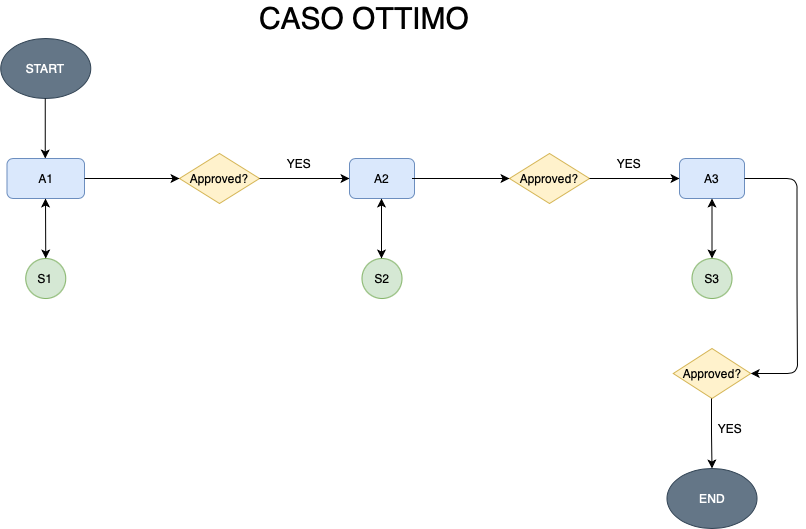
\includegraphics[width=0.50\textwidth,height=\textheight,keepaspectratio]{images/fig_11_1}
\caption{Flow Chart: Caso Ottimo}
\label{fig:6_4}
\end{figure}
\newline
Nella figura [11.1] � rappresentato il flow-chart del caso ottimo, dove si pu� notare che il prodotto entra in fase di lavorazione ed arriva alla fine senza interruzioni e senza alcun rilevamento di anomalie. 
\newline
Nella figura sottostante [11.2] � invece rappresentato il sequence diagram di tutte le operazioni che vengono effettuate dai vari attori della rete. 
\begin{figure}[htbp]
\centering
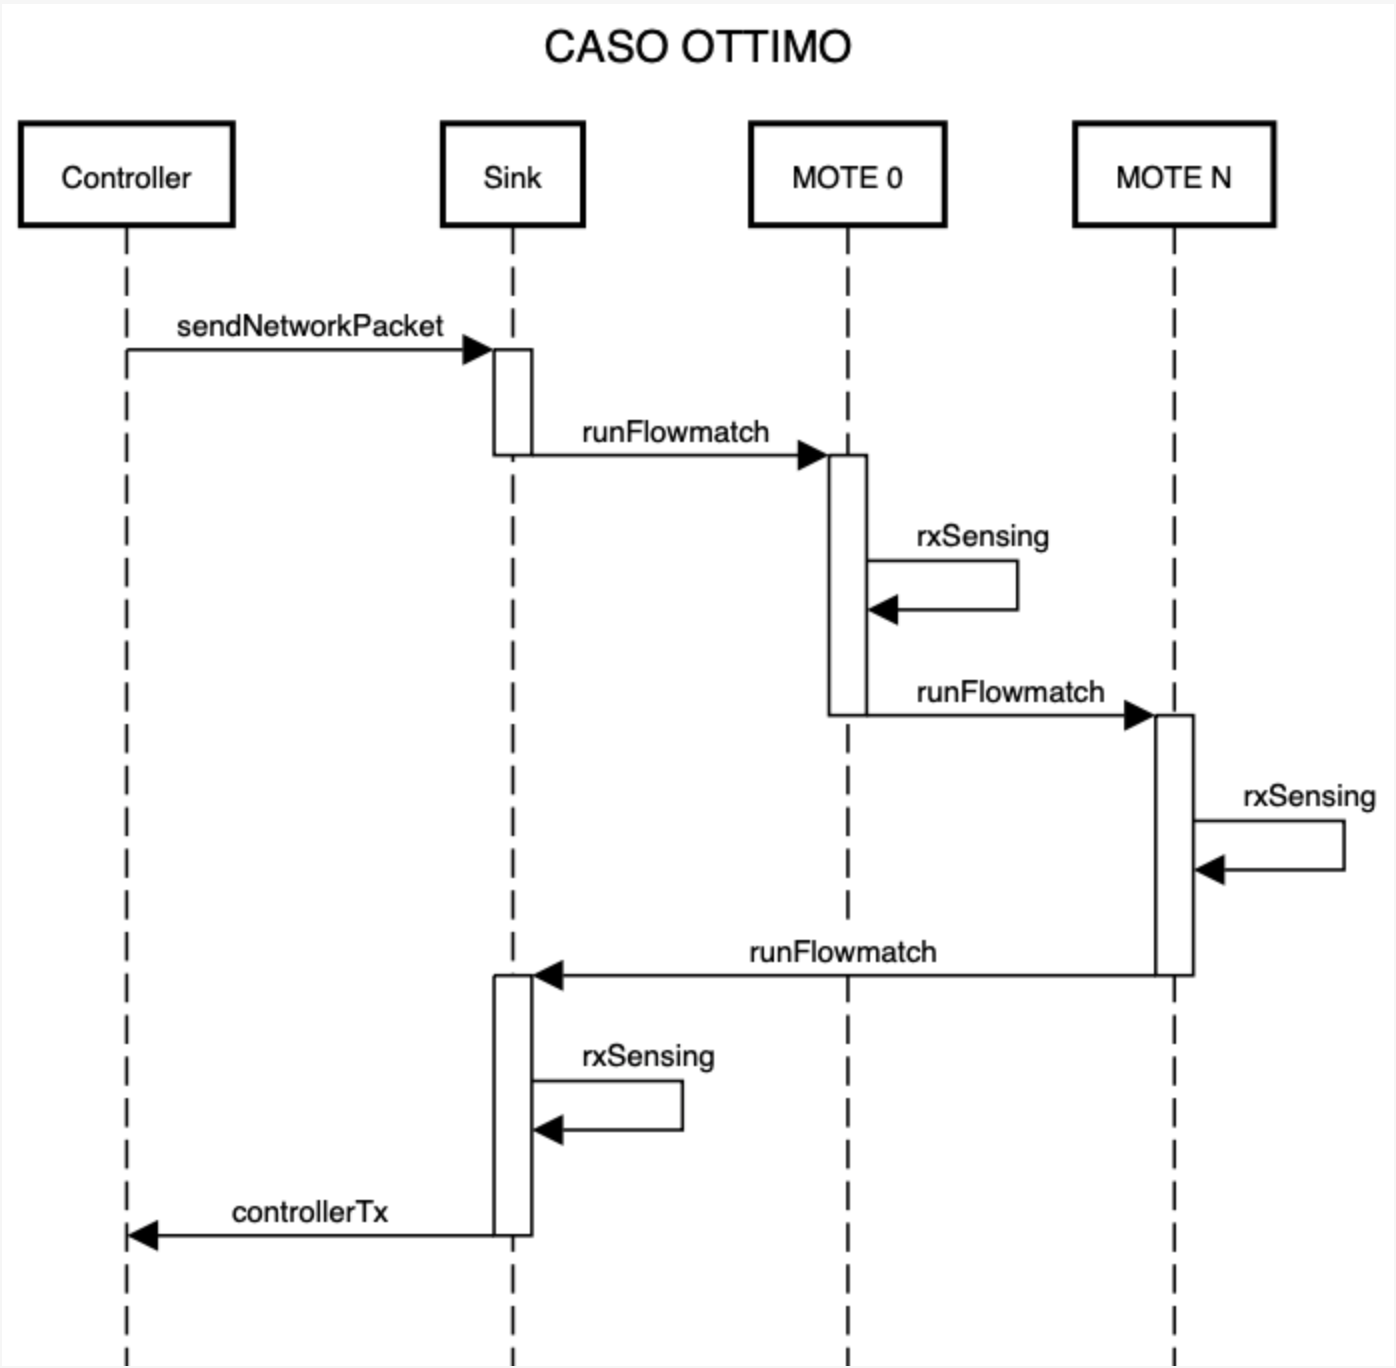
\includegraphics[width=0.70\textwidth,height=\textheight,keepaspectratio]{images/fig_11_2}
\caption{Sequence Diagram: Caso Ottimo}
\label{fig:6_4}
\end{figure}
\newline
Vediamo adesso invece che cosa avviene sulla macchina virtuale, sia all'interno del simulatore Cooja che dentro la console di Intellij IDEA. 
\newline
Di seguito sono riportate le immagini di quello che possiamo leggere all'interno del pannello Mote Output e nella Console di Intellij IDEA. Si noti bene che le simulazioni prese in esempio per le immagini sono con una rete al cui interno sono presenti un Sink, due sensori e due attuatori. 
\begin{figure}[htbp]
\centering
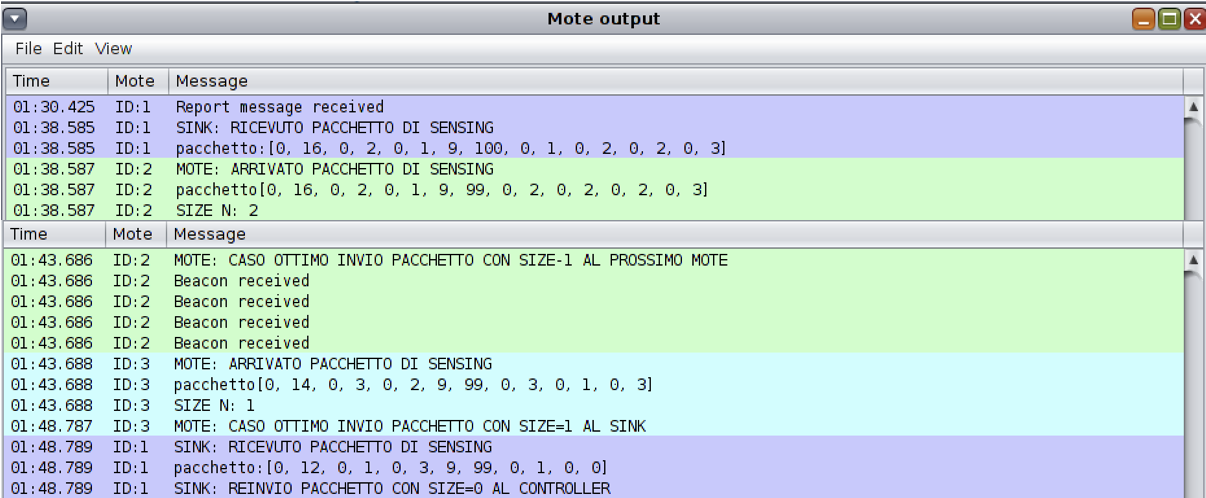
\includegraphics[width=0.60\textwidth,height=\textheight,keepaspectratio]{images/fig_11_3}
\caption{Cooja - Mote Output: Caso Ottimo}
\label{fig:6_4}
\end{figure}

\begin{figure}[htbp]
\centering
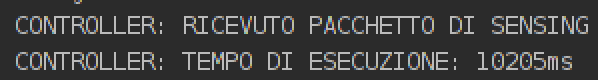
\includegraphics[width=0.60\textwidth,height=\textheight,keepaspectratio]{images/fig_11_4}
\caption{Intellij IDEA - Console: Caso Ottimo}
\label{fig:6_4}
\end{figure}

\subsection{Scenario Caso Pessimo}
Il secondo caso che andremo ad analizzare � il caso pessimo, ovvero quando la catena industriale IoT rileva un'anomalia ed interrompe quindi la lavorazione, scartando il pezzo in lavorazione. 
� sicuramente il caso peggiore che si pu� presentare in fase di lavorazione, poich� oltre ad una perdita di tempo che va ad impattare la produttivit� della catena, abbiamo anche una perdita materiale di risorse poich� il pezzo viene scartato. Il caso pessimo si verifica con una probabilit� del 10\%.

\begin{figure}[htbp]
\centering
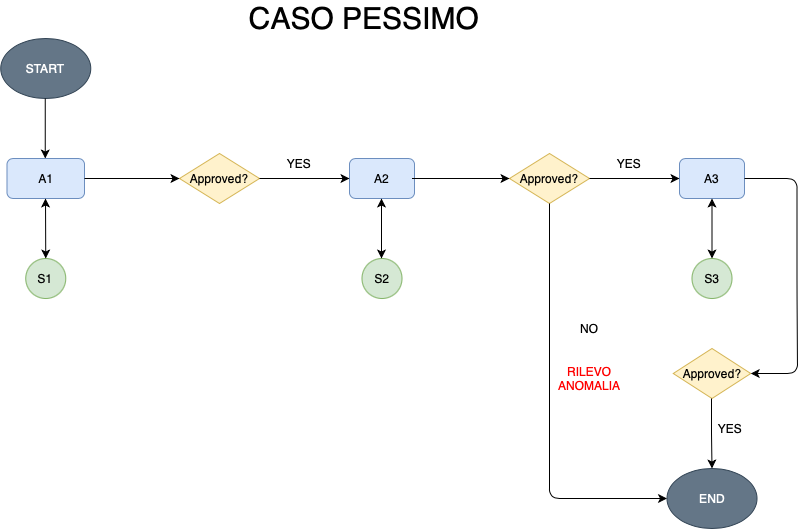
\includegraphics[width=0.50\textwidth,height=\textheight,keepaspectratio]{images/fig_11_5}
\caption{Flow Chart: Caso Pessimo}
\label{fig:6_4}
\end{figure}
Nella figura [11.5] � rappresentato il flow-chart del caso pessimo, dove si pu� notare che il prodotto entra in fase di lavorazione, rileva un'anomalia e termina la lavorazione.
\newline
Nella figura sottostante [11.6] � invece rappresentato il sequence diagram di tutte le operazioni che vengono effettuate dai vari attori della rete. 
\begin{figure}[htbp]
\centering
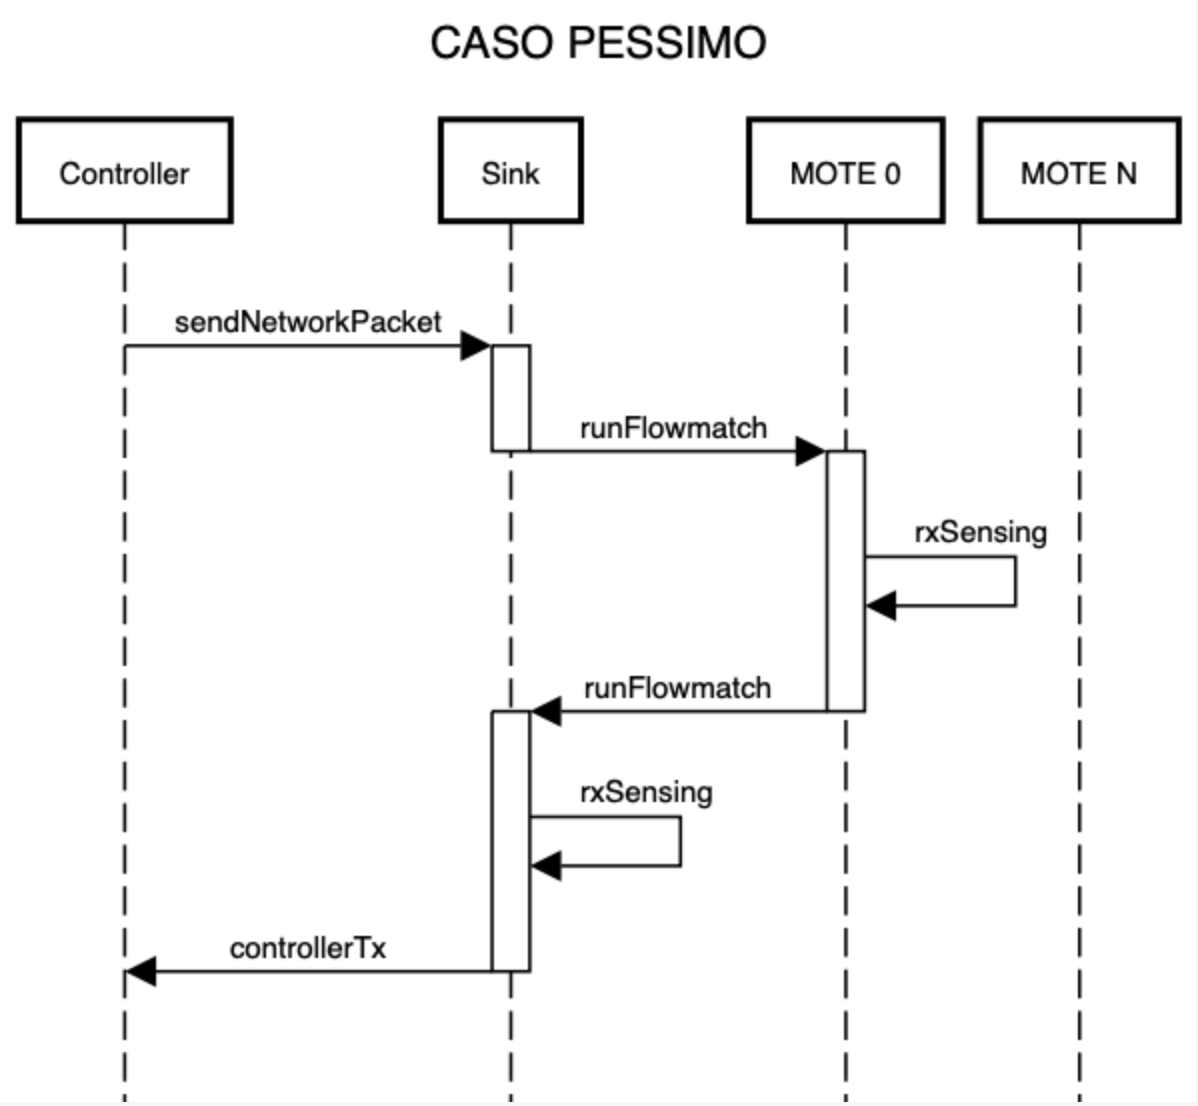
\includegraphics[width=0.70\textwidth,height=\textheight,keepaspectratio]{images/fig_11_6}
\caption{Sequence Diagram: Caso Pessimo}
\label{fig:6_4}
\end{figure}
\newline
Vediamo adesso invece che cosa avviene sulla macchina virtuale, sia all'interno del simulatore Cooja che dentro la console di Intellij IDEA. 
\newline
Di seguito sono riportate le immagini di quello che possiamo leggere all'interno del pannello Mote Output e nella Console di Intellij IDEA. Si noti bene che le simulazioni prese in esempio per le immagini sono con una rete al cui interno sono presenti un Sink, due sensori e due attuatori. 
\begin{figure}[htbp]
\centering
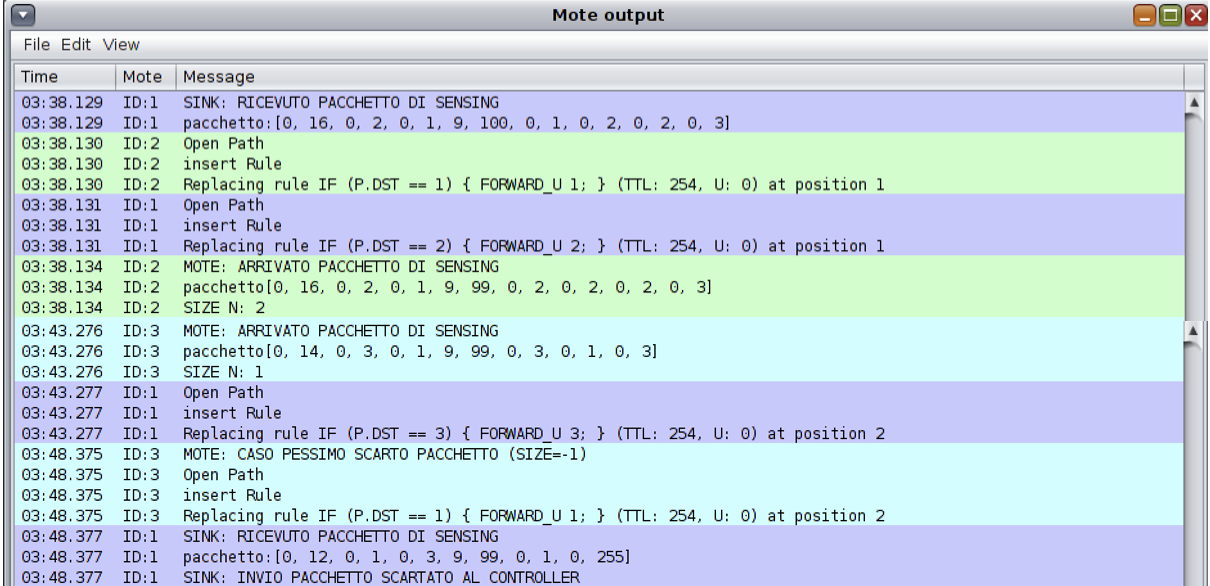
\includegraphics[width=0.60\textwidth,height=\textheight,keepaspectratio]{images/fig_11_7}
\caption{Cooja - Mote Output: Caso Pessimo}
\label{fig:6_4}
\end{figure}

\begin{figure}[htbp]
\centering
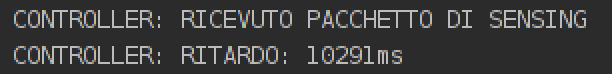
\includegraphics[width=0.60\textwidth,height=\textheight,keepaspectratio]{images/fig_11_8}
\caption{Intellij IDEA - Console: Caso Pessimo}
\label{fig:6_4}
\end{figure}

\subsection{Scenario Caso Intermedio - Restart}
Il terzo caso che andremo ad analizzare � uno dei due casi casi intermedi; in particolare quest'ultimo � stato denominato Restart, poich� quando viene rilevata un'anomalia il pezzo viene rinviato all'inizio della catena di lavorazione e gli viene fatta ripetere tutta la lavorazione fin dal passo iniziale. Questo avviene per permettere una maggiore qualit� ed affidabilit� sulla produzione della catena di montaggio.
\newline
Il caso intermedio Restart si verifica con una probabilit� del 20\%.
\begin{figure}[htbp]
\centering
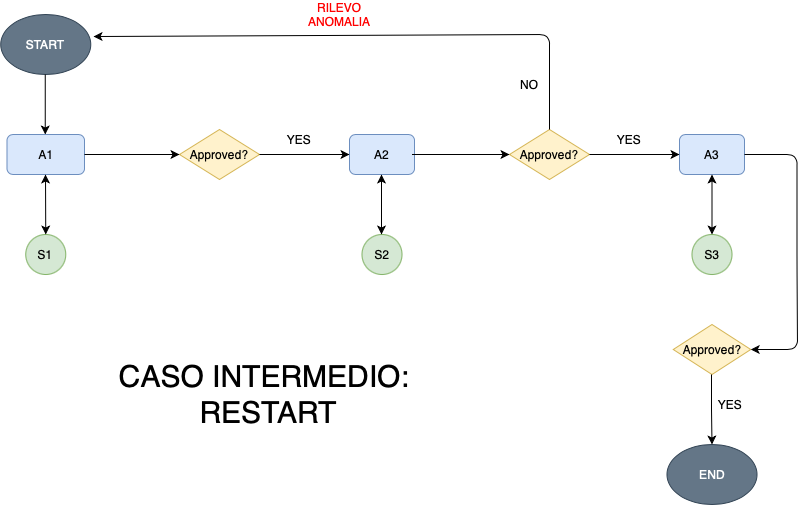
\includegraphics[width=0.50\textwidth,height=\textheight,keepaspectratio]{images/fig_11_9}
\caption{Flow Chart: Caso Intermedio - RESTART}
\label{fig:11_9}
\end{figure}
\newline
Nella figura [11.9] � rappresentato il flow-chart del caso intermedio Restart, dove si pu� notare che il prodotto entra in fase di lavorazione, viene rilevata un'anomalia ed il pezzo viene rinviato all'inizio della catena di montaggio per iniziare nuovamente la lavorazione.
\newline
Nella figura sottostante [11.10] � invece rappresentato il sequence diagram di tutte le operazioni che vengono effettuate dai vari attori della rete. 

\begin{figure}[htbp]
\centering
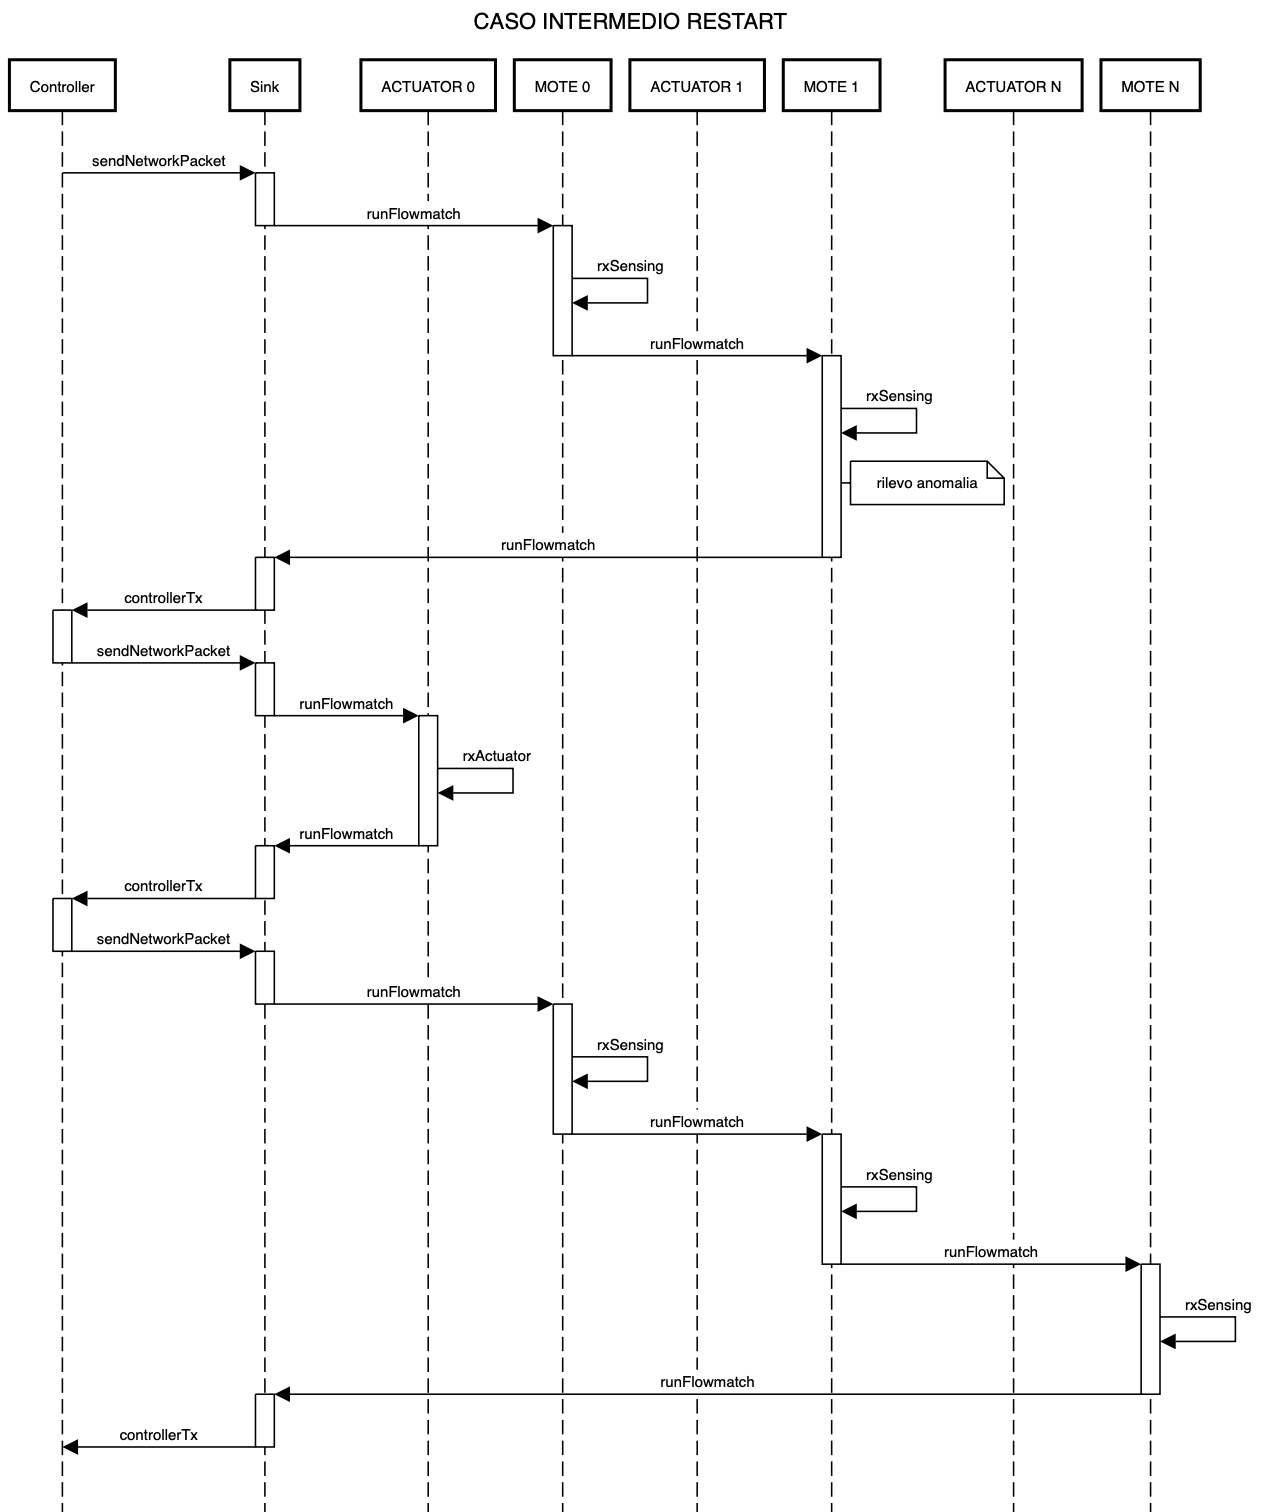
\includegraphics[width=0.70\textwidth,height=\textheight,keepaspectratio]{images/fig_11_10}
\caption{Sequence Diagram: Caso Intermedio RESTART}
\label{fig:6_4}
\end{figure}

Vediamo adesso invece che cosa avviene sulla macchina virtuale, sia all'interno del simulatore Cooja che dentro la console di Intellij IDEA. 
\newline
Di seguito sono riportate le immagini di quello che possiamo leggere all'interno del pannello Mote Output e nella Console di Intellij IDEA. Si noti bene che le simulazioni prese in esempio per le immagini sono con una rete al cui interno sono presenti un Sink, due sensori e due attuatori. 

\begin{figure}[htbp]
\centering
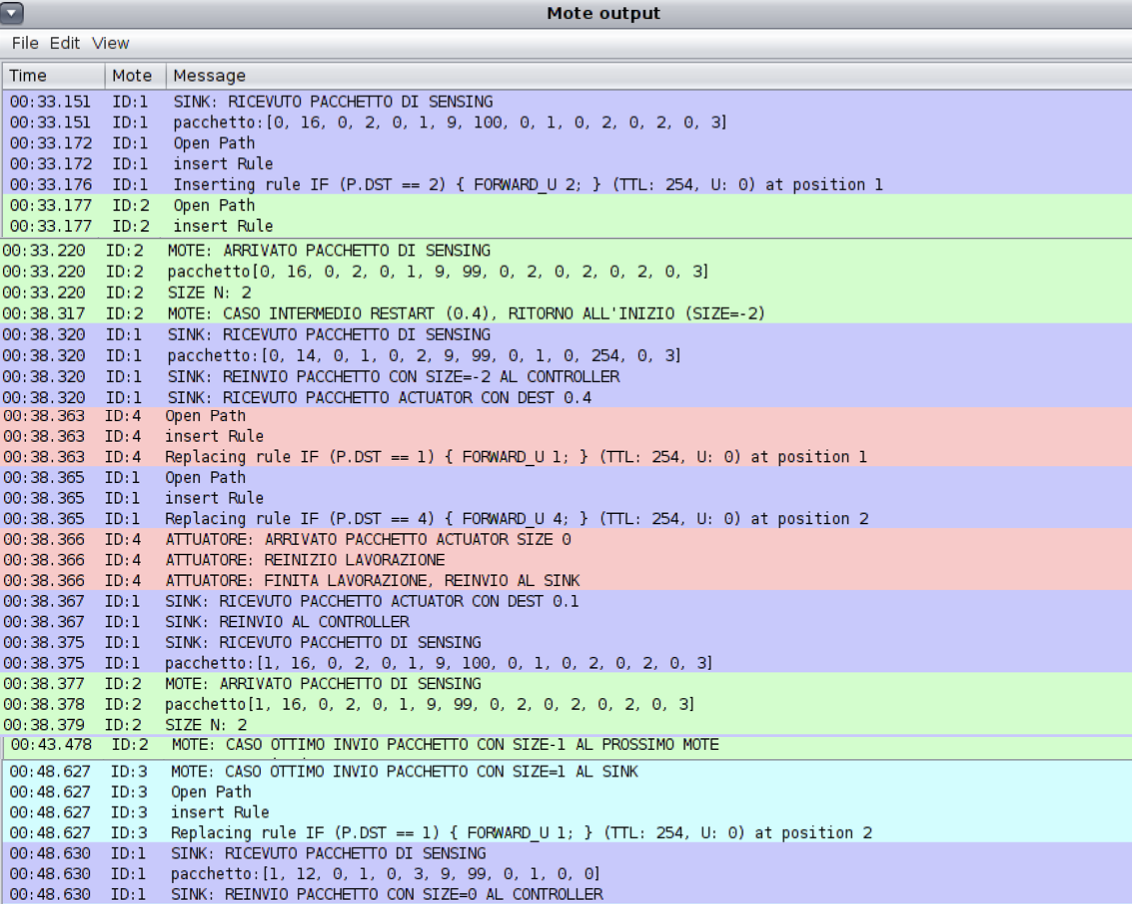
\includegraphics[width=0.60\textwidth,height=\textheight,keepaspectratio]{images/fig_11_11}
\caption{Cooja - Mote Output: Caso Intermedio - Restart}
\label{fig:6_4}
\end{figure}

\begin{figure}[htbp]
\centering
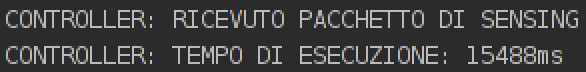
\includegraphics[width=0.60\textwidth,height=\textheight,keepaspectratio]{images/fig_11_12}
\caption{Intellij IDEA - Console: Caso Intermedio - Restart}
\label{fig:6_4}
\end{figure}

\subsection{Scenario Caso Intermedio - Reload}
Il quarto ed ultimo caso che andremo ad analizzare � l'altro caso intermedio; in particolare � stato chiamato Reload, poich� quando viene rilevata un'anomalia, viene fatta ripetere al pezzo quello step di lavorazione dove si � rilevato un qualcosa di anomalo. Questo avviene per permettere una maggiore qualit� ed affidabilit� sulla produzione della catena di montaggio e consente cos� di risparmiare risorse e tempo utile per la produzione.
\newline
Il caso intermedio Reload si verifica con una probabilit� del 30\%.
\newline
\begin{figure}[htbp]
\centering
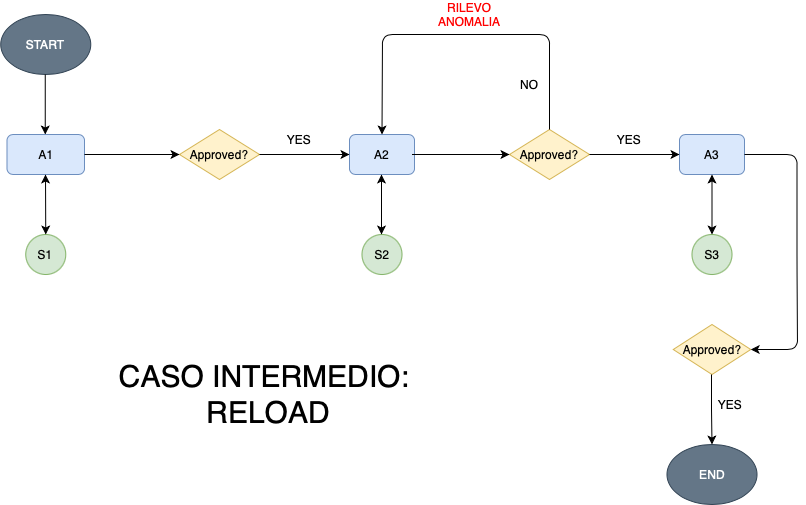
\includegraphics[width=0.60\textwidth,height=\textheight,keepaspectratio]{images/fig_11_13}
\caption{Flow Chart: Caso Intermedio - RELOAD}
\label{fig:6_4}
\end{figure}
Nella figura [11.3] � rappresentato il flow-chart del caso intermedio Restart, dove si pu� notare che il prodotto entra in fase di lavorazione, viene rilevata un'anomalia ed il pezzo viene rinviato all'inizio della catena di montaggio per iniziare nuovamente la lavorazione. Il caso intermedio Reload si verifica con una probabilit� del 30\%.
\begin{figure}[htbp]
\centering
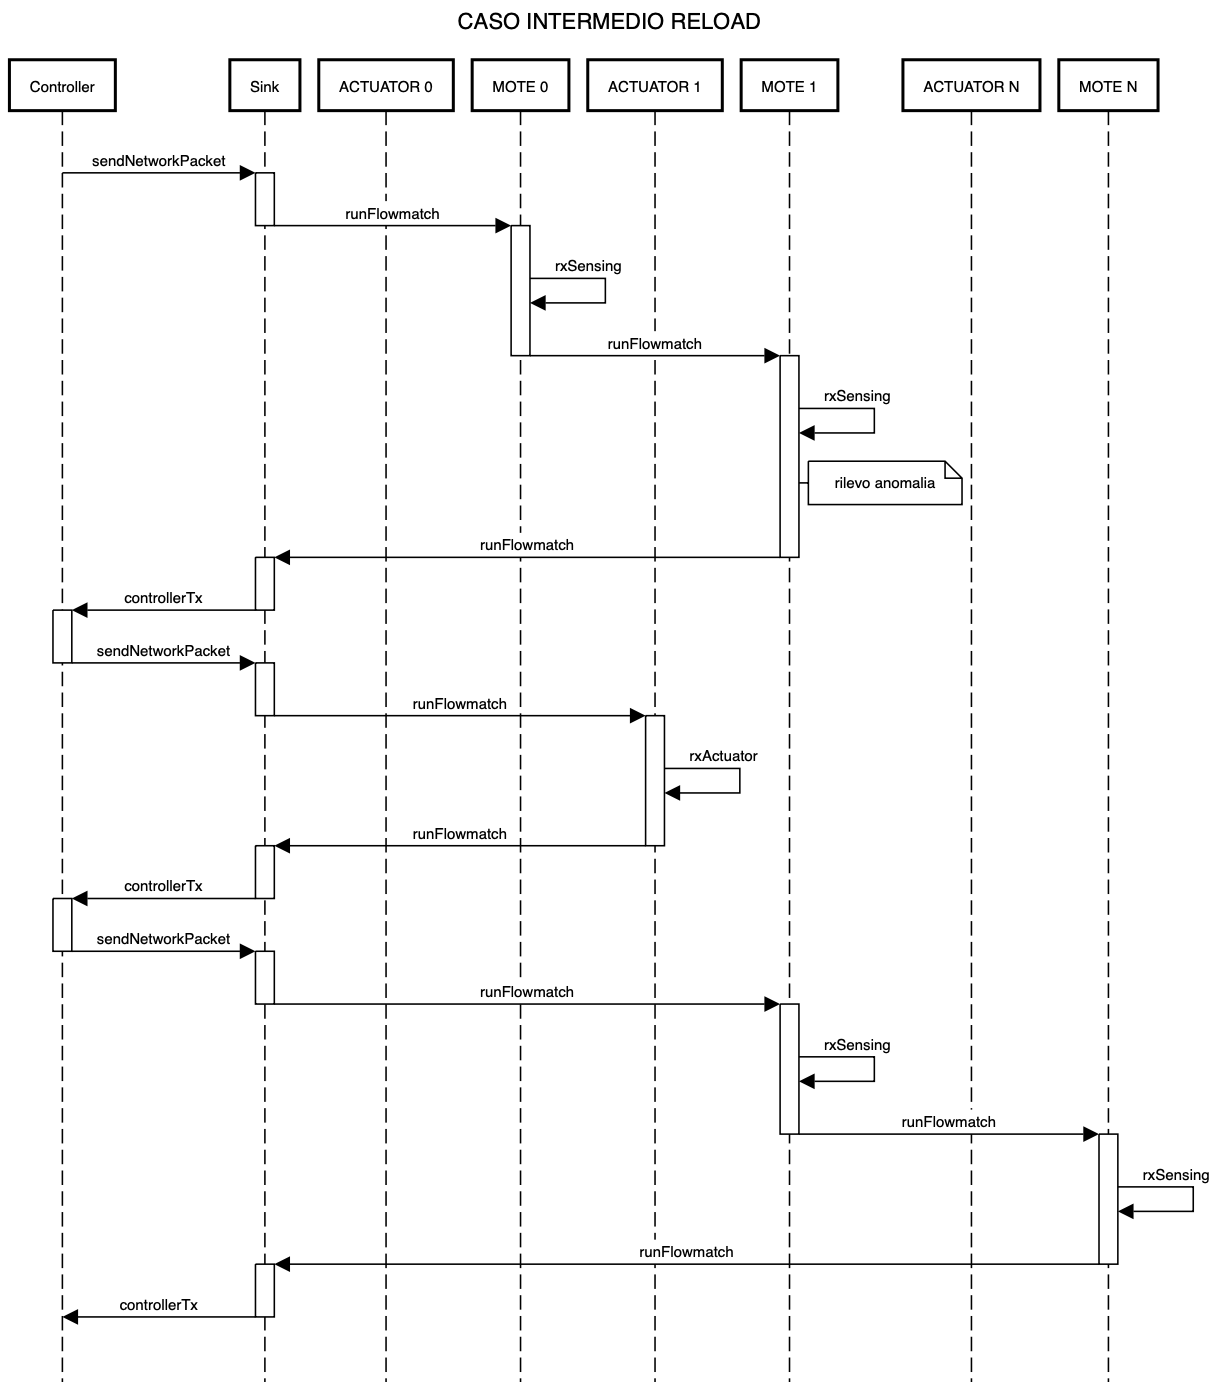
\includegraphics[width=0.60\textwidth,height=\textheight,keepaspectratio]{images/fig_11_14}
\caption{Sequence Diagram: Caso Intermedio RELOAD}
\label{fig:6_4}
\end{figure}
Nella figura sottostante [11.14] � invece rappresentato il sequence diagram di tutte le operazioni che vengono effettuate dai vari attori della rete.
\newline
Vediamo adesso invece che cosa avviene sulla macchina virtuale, sia all'interno del simulatore Cooja che dentro la console di Intellij IDEA. 
\newline
Di seguito sono riportate le immagini di quello che possiamo leggere all'interno del pannello Mote Output e nella Console di Intellij IDEA. Si noti bene che le simulazioni prese in esempio per le immagini sono con una rete al cui interno sono presenti un Sink, due sensori e due attuatori. 

\begin{figure}[htbp]
\centering
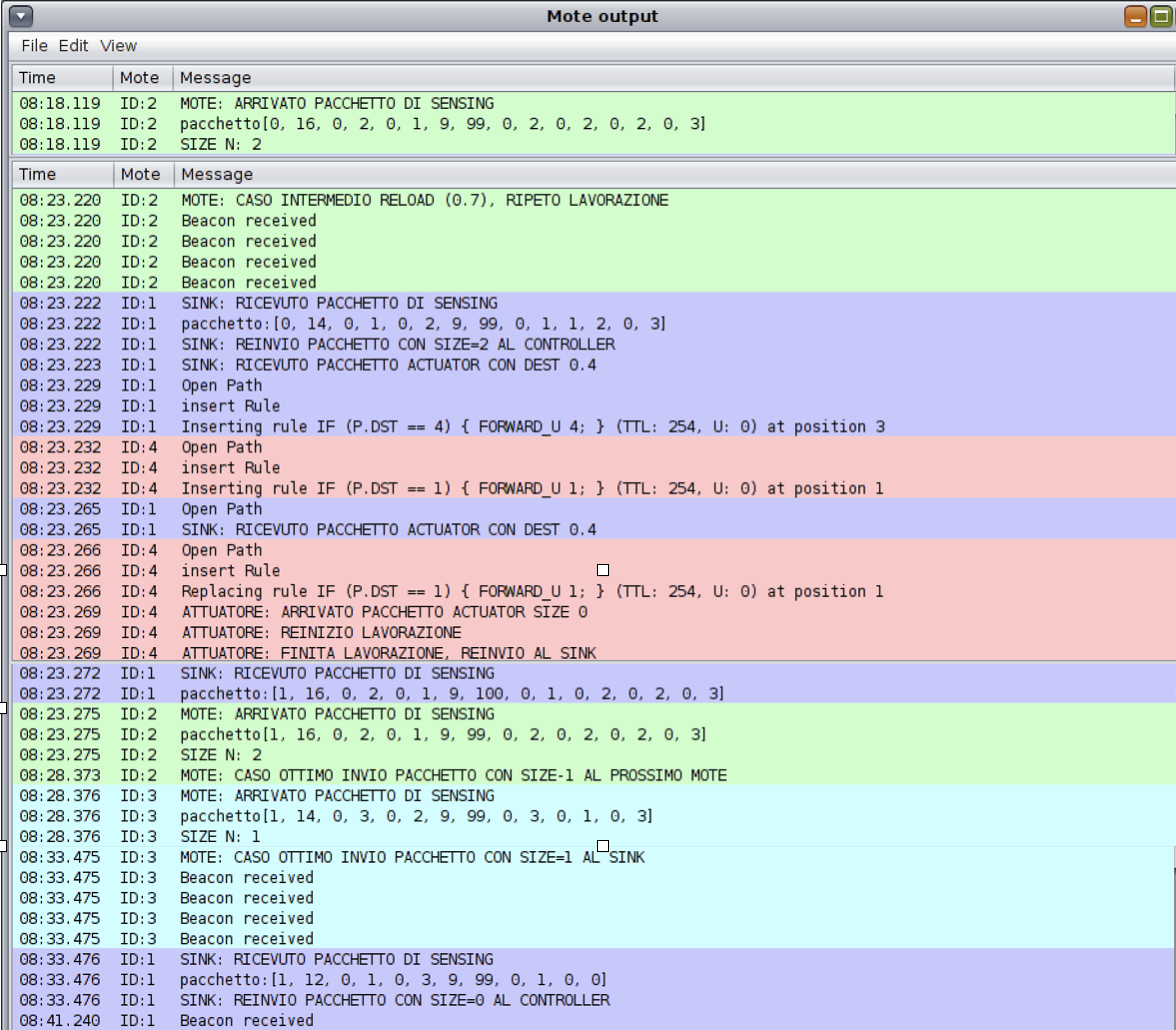
\includegraphics[width=0.60\textwidth,height=\textheight,keepaspectratio]{images/fig_11_15}
\caption{Cooja - Mote Output: Caso Intermedio - Reload}
\label{fig:6_4}
\end{figure}

\begin{figure}[htbp]
\centering
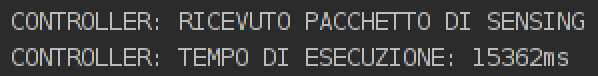
\includegraphics[width=0.60\textwidth,height=\textheight,keepaspectratio]{images/fig_11_16}
\caption{Intellij IDEA - Console: Caso Intermedio - Reload}
\label{fig:6_4}
\end{figure}



\section{Risultati delle simulazioni}
In questa seconda parte del capitolo vedremo i risultati delle simulazioni descritte in precedenza, soffermandoci su un'analisi accurata dei ritardi che i vari casi possono produrre sulla catena industriale IIoT 4.0 e l'impatto che possono avere sulla produzione. 

\subsection{Misurazione del Ritardo}
In questo progetto di catena di montaggio IIoT applicata al paradigma dell'Industria 4.0 � interessante studiare i ritardi che i vari casi implementanti possono generare.
\newline
Prima di fare ci� occorre definire in maniera matematica come � composta la funzione ritardo complessiva, dato che influiscono su di essa molti fattori. In particolare la funzione ritardo � cos� definita:
\newline
\newline
\textit{RITARDO COMPLESSIVO} = \textit{Ritardo Lavorazione} + \textit{Ritardo Lettura Sensore} + \textit{Ritardo Trasmissione}
\newline
\newline
Vediamo adesso nel dettaglio cosa significano le varie voci sui ritardi:
\newline
- \textbf{Ritardo Lavorazione}: questo ritardo � dovuto al tempo che impiega ogni attuatore a svolgere la lavorazione a lui assegnata. Il tempo stimato � di circa 5.0s per ogni step di lavorazione.
\newline
- \textbf{Ritardo Lettura Sensore}: questo ritardo � dovuto al tempo che ogni sensore impiega a leggere i dati sulla lavorazione appena completata. Il ritardo medio � di circa 100ms.
\newline
- \textbf{Ritardo Trasmissione}: questo ritardo � dovuto al tempo che impiegano i vari attori della rete a comunicare fra di loro. Dai dati raccolti, possiamo affermare che in media su una rete composta da un sink, quattro sensori e quattro attuatori il ritardo di trasmissione si attesta fra i 300ms ed i 350ms. Ci aspettiamo quindi che questo aumenti con l'aumentare delle dimensioni della rete.
\newline
Vediamo adesso nello specifico caso per caso. 

\subsubsection{Caso Ottimo}
Il primo caso che valutiamo � proprio il caso ottimo. In questo tipo di simulazione non sono presenti ritardi dato che il pezzo viene lavorato dall'inizio alla fine senza incorrere in anomalie o ricevere interruzioni. Vediamo allora il grafico che raffigura sulle ascisse una catena inizialmente composta da un sink e da un minimo di un attuatore e un sensore fino ad massimo di dieci attuatori e dieci sensori, mentre sulle ordinate il tempo medio dopo dieci prove. 

\begin{figure}[htbp]
\centering
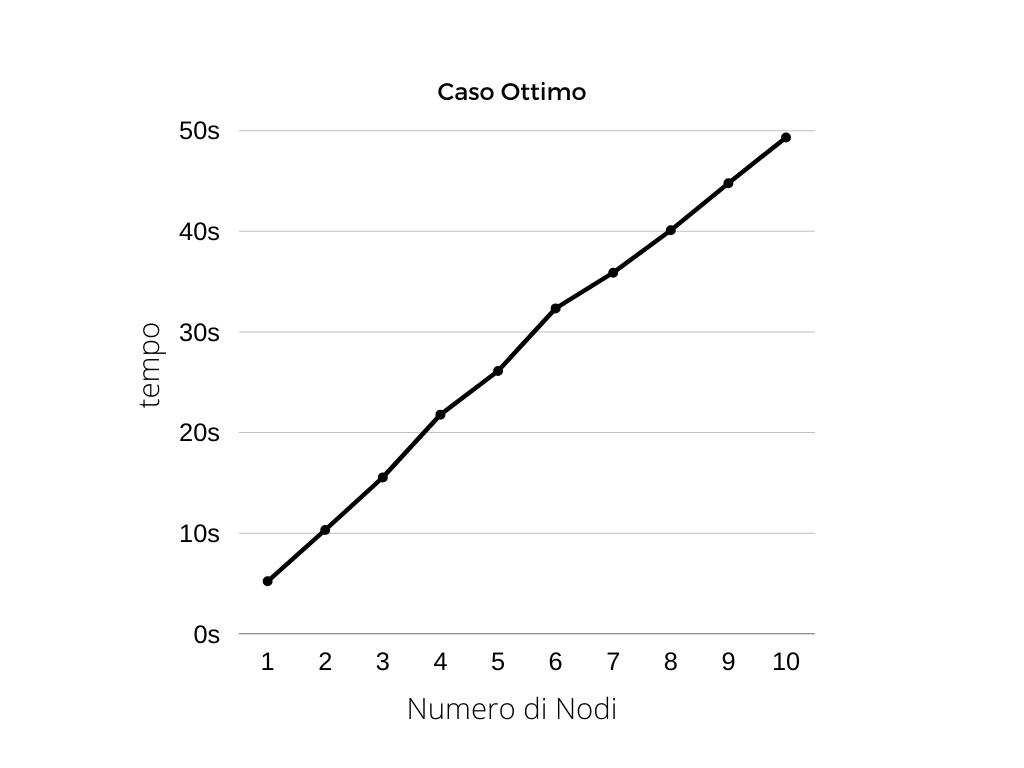
\includegraphics[width=0.80\textwidth,height=\textheight,keepaspectratio]{images/fig_11_17}
\caption{Tempo di esecuzione medio dopo dieci prove}
\label{fig:6_4}
\end{figure}

Come ci potevamo aspettare dalla teoria, questa funzione cresce linearmente al variare del tempo e  con l'aumentare delle dimensioni della rete.

\subsubsection{Caso Pessimo}
Il secondo caso che valutiamo � il caso pessimo. Questo rappresenta sicuramente il caso peggiore che si pu� verificare durante l'esecuzione della catena di montaggio. Infatti ricordiamo che in caso si verifichi il caso pessimo il pezzo viene integralmente scartato; da ci� possiamo quindi dedurre che il tempo di esecuzione sia in realt� tutto ritardo.

\begin{figure}[htbp]
\centering
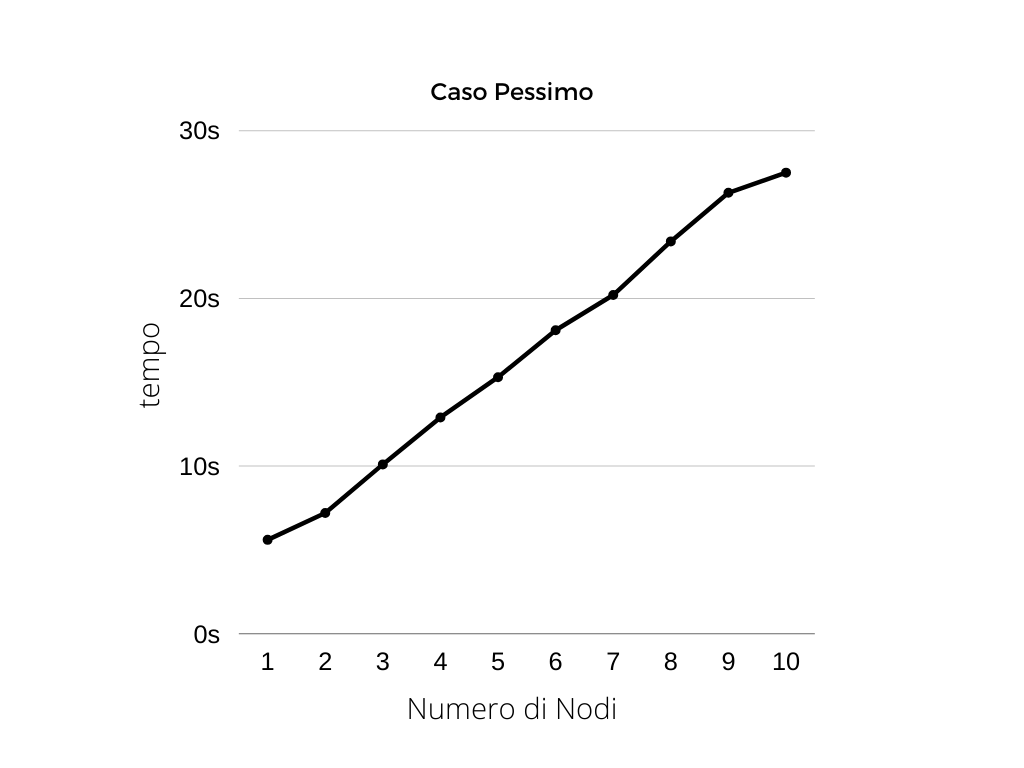
\includegraphics[width=0.80\textwidth,height=\textheight,keepaspectratio]{images/fig_11_18}
\caption{Ritardo Complessivo medio dopo dieci prove}
\label{fig:6_4}
\end{figure}

Anche in questo caso la funzione cresce linearmente, essendo il ritardo nel caso pessimo direttamente proporzionale all'aumentare della rete e al tempo.

\subsubsection{Caso Intermedio - Restart}
Il primo caso intermedio � il caso che abbiamo chiamato \textit{Restart}, ovvero quando durante una lavorazione si rileva una anomalia e si ritorna all'inizio della catena di montaggio, ripetendo la lavorazione. 
\newline
Di seguito � riportato il grafico dove vengono messi a confronto i tempi di esecuzione del caso ottimo e del caso restart.
\begin{figure}[htbp]
\centering
\includegraphics[width=0.80\textwidth,height=\textheight,keepaspectratio]{images/fig_11_19}
\caption{Tempi di Esecuzione a confronto: Ottimo vs Restart}
\label{fig:6_4}
\end{figure}
In particolare il grafico in rosso rappresenta il tempo di esecuzione del caso ottimo, mentre quello in nero il tempo di esecuzione del caso intermedio Restart.
� sicuramente il caso pi� dispendioso e come potevamo aspettarci, all'aumentare delle dimensioni della rete, aumenta il tempo di esecuzione. In particolare la discrepanza che si verifica fra i due casi � quantificabile come ritardo nell'esecuzione della catena di montaggio. 
\newline
Volendo fare una stima e quantificare questo ritardo in secondi, possiamo dire che in media, considerando una rete che varia da uno fino a dieci nodi, e considerando le dieci iterazioni svolte come prova, il ritardo medio � di circa 23,3 secondi.

\subsubsection{Caso Intermedio - Reload}
Nell'ultimo caso analizzato, ovvero il secondo caso intermedio denominato \textit{Reload}, si ha il rilevamento di un'anomalia che comporta la ripetizione dello step di lavorazione dove quest'ultima si � verificata. Infatti il pezzo ripete la lavorazione nel punto in cui era stato fallace, per poi arrivare al termine di tutta la catena di montaggio.
\newline
Di seguito � riportato il grafico dove vengono messi a confronto i tempi di esecuzione del caso ottimo e del caso reload.
\begin{figure}[htbp]
\centering
\includegraphics[width=0.80\textwidth,height=\textheight,keepaspectratio]{images/fig_11_20}
\caption{Tempi di Esecuzione a confronto: Ottimo vs Reload}
\label{fig:6_4}
\end{figure}
In particolare il grafico in rosso rappresenta il tempo di esecuzione del caso ottimo, mentre quello in nero il tempo di esecuzione del caso intermedio Reload. � sicuramente un caso in cui ci aspettiamo del ritardo, ma come si riesce dal leggere dal grafico risulta molto contenuto. Possiamo affermare e quantificare questo ritardo medio, sempre considerando una rete che varia da uno fino a dieci nodi, e considerando le dieci iterazioni svolte come prova, come un ritardo di circa 5.4 secondi.

\subsection{Quantit� prodotte}
In questa ultima parte di capitolo andremo ad analizzare come i vari casi studiati in precedenza vanno ad influenzare le quantit� prodotte da una catena industriale IIoT per l'Industria 4.0, analizzando in forma teorica il rate e la frequenza relativa. Vediamoli adesso pi� nel dettaglio:
\newline
\newline
- \textbf{Rate} = \begin{math}\frac{Numero \quad di \quad Pezzi}{Intervallo \quad temporale}\end{math}
\newline
\newline
Il rate della catena industriale viene calcolato come il numero di pezzi prodotti in un determinato intervallo temporale. Dagli studi fatti possiamo aspettarci che il rate sia massimo nel caso ottimo e che tenda a dimunire negli altri casi, toccando il minimo nel Caso Intermedio Restart, dove ho il ritardo maggiore. Il rate ha come unit� di misura pezzi/secondo.
\newline
\newline
- \textbf{Frequenza Relativa} = \begin{math}{Numero\quad di \quad volte \quad che \quad si \quad verica \quad evento}\over{Numero \quad totale \quad eventi}\end{math}.
\newline
\newline
La formula matematica della frequenza relativa pu� essere utilizzata nella nostra catena industriale, ad esempio, per verificare la frequenza con cui vengono scartati i pezzi rispetto alla frequenza di successo. In questo caso mi aspetto di avere il massimo nel caso ottimo, mentre il minimo sar� chiaramente nel caso pessimo, dove vengono scartati la maggior parte dei pezzi. 





\chapter{Conclusioni}
Dalla visione generale di WSN e SDN, alla loro unione nelle SD-WSN, e in particolare mediante l'architettura SDN-WISE, la comunit� scientifica si aspetta un grande giovamento per il mondo IoT e le azienda stanno investendo molto per uniformarsi agli standard previsti per l'Industria 4.0. Per quanto sperimentato e ottenuto in questa tesi si pu� concludere che la strada � promettente, con l'unico vincolo che il framework SDN-WISE consente di simulare una WSN, ma non verificare nella realt� i risultati ottenuti. Dunque � doveroso, alla luce dei promettenti risultati raccolti, passare a dei veri sensori.
\newline
Da questo progetto di tesi possiamo proporci la domanda, ma SDN ha davvero senso nella sua applicazione industriale? La risposta � ovviamente s�, dato che i vantaggi sono molteplici, ovvero:
\newline
- \textit{Affidabilit�}
\newline
- \textit{Produttivit�}
\newline
- \textit{Sicurezza}
\newline
- \textit{Riduzione dei costi}
\newline
Ovviamente ci sono anche degli aspetti peggiorativi, come ad esempio la non predicibilit� dei vari risultati ottenuti.
\newline
Una possibile soluzione futura � l'introduzione della tecnologia 5G, che in realt� tanto futura non � visto che si parla gi� da molto tempo di questa nuova e rivoluzionaria tecnologia.
\newline
A livello di tempi di risposta si guadagnerebbe in latenza, dato che la latenza per la tecnologia 5G sappiamo essere di 1ms, dato che ha un data-rate molto pi� alto rispetto alle tecnologie attuali. Da ci� possiamo dedurre che quindi il ritardo lettura sensore ed il ritardo di trasmissione riceverebbero una notevole riduzione, aumentando ancora di pi� la produttivit� e diminuendo cos� i ritardi, anche nei casi pi� sfavorevoli.
\newline
Un altro aspetto da considerare della tecnologia 5G � che il Controller SDN ha a disposizione uno scheduler che schedula i vari flussi, alleggerendo di non poco il lavoro al controller.
\newline
\newline
Un possibile sviluppo futuro di questa tesi potrebbe essere, ad esempio, l'introduzione della tecnologia 5G e l'implementazione di pi� controller, per andare poi ad analizzare i dati ottenuti e compararli con la soluzione attuale. 
\newline
\newline
\subsubsection{Ringraziamenti}
Si ringraziano il Professor Francesco Chiti ed il Dottor Michele Bonanni per l'aiuto e la collaborazione forniti durante questi mesi per lo sviluppo di questo progetto di tesi. Nonostante le limitazioni che hanno contraddistinto questo periodo, non hanno fatto mai mancare il loro supporto e la loro volont� di portare a compimento questo progetto innovativo che ha presentato molte sfide durante tutto lo svolgimento. 

% Bibliografia
\addcontentsline{toc}{chapter}{Bibliografia}
\bibliographystyle{ieeetr}
\bibliography{files/bibliografia}

\end{document} 